\documentclass{article}
\usepackage[utf8]{inputenc}
\usepackage[portuguese]{babel}
\usepackage{amsmath, amsthm, amssymb}
\usepackage{graphicx}
\usepackage{listings}
\usepackage{xcolor}
\usepackage{float}

% Define colors for code highlighting
\definecolor{codegreen}{rgb}{0,0.6,0}
\definecolor{codegray}{rgb}{0.5,0.5,0.5}
\definecolor{codepurple}{rgb}{0.58,0,0.82}
\definecolor{backcolour}{rgb}{0.95,0.95,0.92}

% Code style configuration
\lstdefinestyle{mystyle}{
    backgroundcolor=\color{backcolour},
    commentstyle=\color{codegreen},
    keywordstyle=\color{magenta},
    numberstyle=\tiny\color{codegray},
    stringstyle=\color{codepurple},
    basicstyle=\ttfamily\footnotesize,
    breakatwhitespace=false,
    breaklines=true,
    captionpos=b,
    keepspaces=true,
    numbers=left,
    numbersep=5pt,
    showspaces=false,
    showstringspaces=false,
    showtabs=false,
    tabsize=2
}

\lstset{style=mystyle}

\title{Lista 02 - Machine Learning\\
IMPA}
\author{Pedro Barbosa Bahia}
\date{\today}

\begin{document}

\maketitle
\newpage
\tableofcontents
\newpage

% Include all exercise files
\section*{Exercício 1}
\addcontentsline{toc}{section}{Exercício 1}

\subsection*{Exercício 1a}
\addcontentsline{toc}{subsection}{Exercício 1a}
\subsection*{Item a}
\addcontentsline{toc}{subsection}{Item a}
A partir da função de custo para Ridge Regression:
$$ L = \sum_{i=1}^n \left( y_i - \beta_0 - \sum_{j=1}^p x_{ij}\beta_j \right)^2 + \lambda \sum_{j=1}^p \beta_j^2 $$

Derivando em relação a $ \beta_0 $ e igualando a zero, temos:
$$ \frac{\partial L}{\partial \beta_0} = \sum_{i=1}^n 2 \left( y_i - \beta_0 - \sum_{j=1}^p x_{ij}\beta_j \right) (-1) = 0 $$
$$ -2 \sum_{i=1}^n \left( y_i - \beta_0 - \sum_{j=1}^p x_{ij}\beta_j \right) = 0 $$
$$ \sum_{i=1}^n y_i - n\beta_0 - \sum_{i=1}^n \sum_{j=1}^p x_{ij}\beta_j = 0 $$

Isolando $ \beta_0 $:
$$ \beta_0 = \frac{1}{n}\sum_{i=1}^n y_i - \frac{1}{n}\sum_{i=1}^n \sum_{j=1}^p x_{ij}\beta_j $$
$$ \beta_0 = \bar{y} - \sum_{j=1}^p \bar{x}_j \beta_j $$

Caso os dados estejam centralizados, teremos $ \bar{y} = 0 $ e $ \bar{x}_j = 0 $. Portanto, $ \hat{\beta}_0 = 0 $.


\newpage

\subsection*{Exercício 1b}
\addcontentsline{toc}{subsection}{Exercício 1b}
A função de custo na forma matricial, com $ \beta_0 $ = 0, é:
$$ L = (Y - X\beta)^T(Y - X\beta) + \lambda \beta^T\beta $$

Derivando em relação ao vetor $ \beta $ e igualando a zero, temos:
$$ \frac{\partial L}{\partial \beta} = -2X^T(Y - X\beta) + 2\lambda\beta = 0 $$
$$ -X^T Y + X^T X \beta + \lambda\beta = 0 $$
$$ (X^T X + \lambda I)\beta = X^T Y $$

O estimador em forma fechada é:
$$ \hat{\beta} = (X^T X + \lambda I)^{-1}X^T Y $$






Assumindo que $ \lambda \to 0 $, o termo de regularização desaparece e temos:
$$ \hat{\beta} = (X^T X)^{-1}X^T Y $$
que é a fórmula fechada clássica para a Regressão Linear sem regularização.


\newpage

\subsection*{Exercício 1c}
\addcontentsline{toc}{subsection}{Exercício 1c}
\subsection*{Item c}
\addcontentsline{toc}{subsection}{Item c}
A partir do estimador em forma fechada encontrado no item (b):
$$ \hat{\beta} = (X^T X + \lambda I)^{-1}X^T Y $$
$$ = (\lambda I + X^T I X)^{-1} X^T Y$$

$$ = \left[(\lambda I)^{-1} - (\lambda I)^{-1}X^T(I + X(\lambda I)^{-1}X^T)^{-1}X(\lambda I)^{-1} \right] X^T Y $$
$$ = \left[\frac{1}{\lambda}I - \frac{1}{\lambda}X^T \left(I + \frac{1}{\lambda}XX^T \right)^{-1} X\frac{1}{\lambda} \right] X^T Y $$
$$ = \frac{1}{\lambda} \left[ X^T - X^T \left(I + \frac{1}{\lambda}XX^T \right)^{-1} \left(\frac{1}{\lambda}XX^T \right) \right] Y $$
$$ = \frac{1}{\lambda} X^T \left[ I - \left(I + \frac{1}{\lambda}XX^T \right)^{-1} \left(\frac{1}{\lambda}XX^T \right) \right] Y $$
$$ = \frac{1}{\lambda} X^T \left[ I - \left(I + \frac{1}{\lambda}XX^T \right)^{-1} \left(I + \frac{1}{\lambda}XX^T - I \right) \right] Y $$
$$ = \frac{1}{\lambda} X^T \left[ I - I + \left(I + \frac{1}{\lambda}XX^T \right)^{-1} \right] Y $$
$$ = X^T \left[ \frac{1}{\lambda} \left(I + \frac{1}{\lambda}XX^T \right)^{-1} Y \right] $$

Portanto, podemos escrever $ \hat{\beta} = X^T \alpha $, onde o vetor $ \alpha $ é dado por:
$$ \alpha = \frac{1}{\lambda} \left(I + \frac{1}{\lambda}XX^T \right)^{-1} Y $$
$$ \alpha = \left( \lambda I + XX^T \right)^{-1} Y $$

\newpage

\subsection*{Exercício 1d}
\addcontentsline{toc}{subsection}{Exercício 1d}
\subsection*{Item d}
\addcontentsline{toc}{subsection}{Item d}
Para um novo ponto $ x^* $, a previsão $ \hat{y}^* $ é:
$$ \hat{y}^* = (x^*)^T \hat{\beta} $$

Substituindo $ \hat{\beta} = X^T \alpha $ encontrado no item (c):
$$ \hat{y}^* = (x^*)^T X^T \alpha $$

Sabendo que $ X^T = [x_1, x_2, \dots, x_n] $, o produto pode ser expresso como uma combinação linear de produtos internos:
$$ \hat{y}^* = \sum_{i=1}^n \alpha_i (x^*)^T x_i $$

\newpage

\subsection*{Exercício 1e}
\addcontentsline{toc}{subsection}{Exercício 1e}
\subsection*{Item e}
\addcontentsline{toc}{subsection}{Item e}
Para "kernelizarmos" a previsão do modelo Ridge Regression, basta substituir o produto interno $ (x^*)^T x_i $ por uma função de kernel arbitrária $ K(x^*, x_i) $, que computa o produto interno em um espaço de características de alta dimensão. Assim, a fórmula de previsão se torna:
$$ \hat{y}^* = \sum_{i=1}^n \alpha_i K(x^*, x_i) $$


\newpage

\subsection*{Exercício 1f}
\addcontentsline{toc}{subsection}{Exercício 1f}
\subsection*{Item f}
\addcontentsline{toc}{subsection}{Item f}
No cálculo da função de custo e na otimização do SVM, apenas os vetores de
suporte são considerados. Pelas condições de KKT, temos que $ \alpha_i > 0 $
apenas para os pontos onde a restrição de margem é ativa, ou seja, onde
$ y_i(w^T x_i + \beta) = 1 $ (os vetores de suporte). Para todas as outras
amostras, $ \alpha_i = 0 $. Isso faz com que o vetor $ \alpha $ no SVM seja
altamente esparso.

Enquanto isso, na Ridge Regression, os valores de $ \alpha_i $ calculados raramente serão nulos.
De modo que a quase totalidade das amostras de treino contribuirá para a
soma final da previsão $ \hat{y}^* $. Devido à esparsidade do vetor
$ \alpha $ no SVM, ele se torna computacionalmente mais eficiente..

\newpage

\subsection*{Exercício 1g}
\addcontentsline{toc}{subsection}{Exercício 1g}



\begin{lstlisting}[language=Python]
import numpy as np
import pandas as pd
from sklearn.model_selection import train_test_split, KFold
from sklearn.linear_model import Ridge, LinearRegression
from sklearn.kernel_ridge import KernelRidge
from sklearn.pipeline import make_pipeline
from sklearn.preprocessing import StandardScaler
from tqdm import tqdm
from sklearn.metrics import mean_squared_error

number_of_folds = 10
data = pd.read_csv("../data/bodyfat.csv")
X = data.drop(columns=["BodyFat", "Density"])
y = data["BodyFat"]
X_train, X_test, y_train, y_test = train_test_split(
    X, y, test_size=0.2, random_state=0
    )
\end{lstlisting}
\newpage
\subsubsection*{(i) Erro médio quadrático da regressão linear}

\begin{lstlisting}[language=Python]
linear_regression_model = LinearRegression(fit_intercept=True)
linear_regression_model.fit(X_train, y_train)
y_hat = linear_regression_model.predict(X_test)
mse_linear = mean_squared_error(y_true=y_test, y_pred=y_hat)

y_hat_train = linear_regression_model.predict(X_train)
mse_linear_train = mean_squared_error(y_true=y_train, y_pred=y_hat_train)
\end{lstlisting}
\begin{table}[h!]
    \centering
    \begin{tabular}{|l|c|}
        \hline
        Conjunto & Erro médio quadrático       \\ \hline
        Teste    & \textbf{15.910489104854445} \\
        Treino   & \textbf{18.090133641655044} \\
        \hline
    \end{tabular}
    \caption{Resultados da regressão linear}
\end{table}
\newpage
\subsubsection*{(ii) Erro médio quadrático da regressão ridge}

\begin{lstlisting}[language=Python]
alphas = 10 ** np.linspace(3, -2, 100)
ridge_cv_mse = []
for alpha in tqdm(alphas):
    cv_MSE = []
    folds = KFold(
        n_splits=number_of_folds, shuffle=True, random_state=2023
    ).split(X_train, y_train)

    for train_idx, val_idx in folds:
        ridge_pipeline = make_pipeline(
            StandardScaler(), Ridge(alpha=alpha)
        )
        ridge_pipeline.fit(
            X_train.iloc[train_idx], y_train.iloc[train_idx]
        )
        y_hat = ridge_pipeline.predict(
            X_train.iloc[val_idx]
        )
        cv_MSE.append(
            mean_squared_error(y_true=y_train.iloc[val_idx], y_pred=y_hat)
        )

    ridge_cv_mse.append(np.mean(cv_MSE))

optimal_alpha = alphas[np.argmin(ridge_cv_mse)]
ridge_pipeline = make_pipeline(
    StandardScaler(), Ridge(alpha=optimal_alpha)
)
ridge_pipeline.fit(X_train, y_train)
y_hat_ridge = ridge_pipeline.predict(X_test)
ridge_test_mse = mean_squared_error(y_true=y_test, y_pred=y_hat_ridge)

y_hat_ridge_train = ridge_pipeline.predict(X_train)
ridge_train_mse = mean_squared_error(
    y_true=y_train, y_pred=y_hat_ridge_train
)
\end{lstlisting}

O melhor valor de $\alpha$ encontrado foi \textbf{0.52}. Com ele, obteve-se os seguintes erros médios
quadráticos:

\begin{table}[h!]
    \centering
    \begin{tabular}{|l|c|}
        \hline
        Conjunto             & Erro médio quadrático \\ \hline
        Validação (10 folds) & \textbf{21.84}        \\
        Teste                & \textbf{15.87}        \\
        Treino               & \textbf{18.099}       \\
        \hline
    \end{tabular}
    \caption{Resultados da regressão ridge}
\end{table}
\newpage
\subsubsection*{(iii) Kernel para Ridge Regression}

\begin{lstlisting}[language=Python]
kernels = ["linear", "polynomial", "rbf", "laplacian"]
gammas = [10**-3]
alphas = 10 ** np.linspace(3, -2, 100)
hyperparams = [
    (kernel, gamma, alpha)
    for kernel in kernels
    for gamma in gammas
    for alpha in alphas
]

kernel_ridge_cv_mse = []
for hyperparam in tqdm(hyperparams):
    kernel_fold, gamma_fold, alpha_fold = hyperparam
    cv_MSE = []
    folds = KFold(
        n_splits=number_of_folds, shuffle=True, random_state=2023
    ).split(X_train, y_train)

    for train_idx, val_idx in folds:
        kernel_ridge_pipeline = make_pipeline(
            StandardScaler(),
            KernelRidge(
                kernel=kernel_fold, 
                alpha=alpha_fold,
                gamma=gamma_fold
            ),
        )
        kernel_ridge_pipeline.fit(
            X_train.iloc[train_idx], y_train.iloc[train_idx]
        )
        y_hat = kernel_ridge_pipeline.predict(X_train.iloc[val_idx])
        cv_MSE.append(
            mean_squared_error(y_true=y_train.iloc[val_idx], y_pred=y_hat)
        )

    kernel_ridge_cv_mse.append(np.mean(cv_MSE))

optimal_hyperparam = hyperparams[np.argmin(kernel_ridge_cv_mse)]
optimal_kernel, optimal_gamma, optimal_alpha = optimal_hyperparam

kernel_ridge_pipeline = make_pipeline(
    StandardScaler(),
    KernelRidge(
        kernel=optimal_kernel, alpha=optimal_alpha, gamma=optimal_gamma
    ),
)
kernel_ridge_pipeline.fit(X_train, y_train)
kernel_y_hat_ridge = kernel_ridge_pipeline.predict(X_test)
kernel_ridge_test_mse = mean_squared_error(
    y_true=y_test, y_pred=kernel_y_hat_ridge
)

kernel_y_hat_ridge_train = kernel_ridge_pipeline.predict(X_train)
kernel_ridge_train_mse = mean_squared_error(
    y_true=y_train, y_pred=kernel_y_hat_ridge_train
)
\end{lstlisting}

O melhor conjunto de hiperparâmetros encontrado é:
este é: 14.66379896222263
reino é: 17.223450675066484

\begin{table}[h!]
    \centering
    \begin{tabular}{|c|c|}
        \hline
        Hiperparâmetro & Valor          \\ \hline
        $\alpha$       & \textbf{0.01}  \\
        $\gamma$       & \textbf{0.001} \\
        kernel         & \textbf{rbf}   \\ \hline
    \end{tabular}
\end{table}

Com ele, os erros médios encontrados foram:
\begin{table}[h!]
    \centering
    \begin{tabular}{|l|c|}
        \hline
        Conjunto             & Erro médio quadrático \\ \hline
        Validação (10 folds) & \textbf{20.55}        \\
        Teste                & \textbf{14.66}        \\
        Treino               & \textbf{17.22}        \\
        \hline
    \end{tabular}
    \caption{Resultados da regressão ridge com kernel}
\end{table}


\newpage
\subsubsection*{(iv) Comparação dos modelos}

\textbf{Resultados no conjunto de treino:}
\begin{table}[h!]
    \centering
    \begin{tabular}{|l|c|}
        \hline
        Modelo                     & Erro médio quadrático \\ \hline
        Regressão linear           & \textbf{18.09}        \\
        Regressão ridge            & \textbf{18.53}        \\
        Regressão ridge com kernel & \textbf{17.22}        \\
        \hline
    \end{tabular}
    \caption{Resultados de treino}
\end{table}

\textbf{Resultados no conjunto de teste:}
\begin{table}[h!]
    \centering
    \begin{tabular}{|l|c|}
        \hline
        Modelo                     & Erro médio quadrático \\ \hline
        Regressão linear           & \textbf{15.91}        \\
        Regressão ridge            & \textbf{15.87}        \\
        Regressão ridge com kernel & \textbf{14.66}        \\
        \hline
    \end{tabular}
    \caption{Resultados de teste}
\end{table}

Dos três modelos analizados, o que apresentou melhor desempenho foi a regressão ridge com kernel, tanto no conjunto de treino quanto no conjunto de teste. A
regressão linear e a regressão ridge apresentaram desempenhos semelhantes, com a regressão ridge tendo um desempenho ligeiramente pior no conjunto de treino,
mas melhor no conjunto de teste. Isso sugere que a regressão ridge pode ter ajudado a reduzir o overfitting em comparação com a regressão linear,
enquanto a adição do kernel na regressão ridge permitiu capturar relações não lineares nos dados, resultando em um desempenho superior.
\newpage

\section*{Exercício 2}
\addcontentsline{toc}{section}{Exercício 2}

\subsection*{Exercício 2a}
\addcontentsline{toc}{subsection}{Exercício 2a}
\subsection*{(a) Minimização da Perda e Relações de $L_t$}
\addcontentsline{toc}{subsection}{(a) Minimização da Perda e Relações de $L_t$}
A função de perda no passo $t$ pode ser dividida entre as amostras classificadas corretamente e incorretamente:
\begin{equation*}
    L_t(\tilde{\alpha}, \tilde{\theta}) = \sum_{i: \tilde{y}_i = F} w_{it} e^{-\tilde{\alpha}} + \sum_{i: \tilde{y}_i \neq F} w_{it} e^{\tilde{\alpha}}
\end{equation*}
Podemos simplificar utilizando as definições dadas para os pesos:
\begin{equation*}
    L_t(\tilde{\alpha}, \tilde{\theta}) = e^{-\tilde{\alpha}}W_t^{=} + e^{\tilde{\alpha}}W_t^{\neq}
\end{equation*}
Para encontrar o mínimo, derivamos em relação a $\alpha$ e igualamos a zero:
\begin{equation*}
    \frac{dL}{d\alpha} = -e^{-\alpha} W_t^{=} + e^{\alpha} W_t^{\neq} = 0
\end{equation*}
Elevando ao quadrado ambos os lados e somando o termo 4$W_t^{=}W_t^{\neq}$ para manter a igualdade, obtemos:
\begin{equation*}
    (e^{\alpha} W_t^{\neq})^2 + 2W_t^{=}W_t^{\neq} + (e^{-\alpha}W_t^{=})^2 = 4W_t^{=}W_t^{\neq}
\end{equation*}
\begin{equation*}
    (e^{\alpha} W_t^{\neq} + e^{-\alpha} W_t^{=})^2 = 4W_t^{=}W_t^{\neq}
\end{equation*}
\begin{equation*}
    e^{\alpha} W_t^{\neq} + e^{-\alpha} W_t^{=} = 2\sqrt{W_t^{=}W_t^{\neq}}
\end{equation*}

Substituindo a relação na equação de perda, obtemos o valor mínimo:
\begin{equation*}
    L_t(\hat{\alpha}_t, \hat{\theta}_t) = \min_{\tilde{\alpha}} L_t(\tilde{\alpha}, \hat{\theta}_t) = 2\sqrt{W_t^{=} \cdot W_t^{\neq}}
\end{equation*}

Para $L_{t-1}$, avaliando a perda acumulada (equivalente a avaliar $\alpha = 0$ antes da atualização), temos a soma dos pesos:
\begin{equation*}
    L_{t-1}(\hat{\alpha}_{t-1}, \hat{\theta}_{t-1}) = \sum W_i = W_t^{=} + W_t^{\neq}
\end{equation*}

\newpage

\subsection*{Exercício 2b}
\addcontentsline{toc}{subsection}{Exercício 2b}

\subsection*{(b) Limite Superior para o Erro com Algoritmo Fraco}
\addcontentsline{toc}{subsection}{(b) Limite Superior para o Erro com Algoritmo Fraco}
Pela definição de algoritmo fraco, existirá um $\hat{\theta}$ tal que, para qualquer distribuição de probabilidade, o erro é menor ou igual a $\frac{1}{2} - \gamma$.
Definindo a probabilidade $p_i = \frac{w_i}{\sum w_i}$ e sabendo que a soma dos pesos é $\sum w_i = W_t^{=} + W_t^{\neq}$, temos:
\begin{equation*}
    \sum_{i} \frac{w_i}{W_t^{=} + W_t^{\neq}} \mathbb{I}_{[F(x_i, \hat{\theta}) \neq \tilde{y}_i]} \le \frac{1}{2} - \gamma
\end{equation*}
O que nos leva à expressão:
\begin{equation*}
    \frac{1}{W_t^{=} + W_t^{\neq}} \sum_{\tilde{y}_i \neq F(x_i, \hat{\theta})} w_i \le \frac{1}{2} - \gamma
\end{equation*}


\newpage

\subsection*{Exercício 2c}
\addcontentsline{toc}{subsection}{Exercício 2c}
\subsection*{(c)}
\addcontentsline{toc}{subsection}{(c)}
Temos que
\[
    W_t^{\neq} = \sum_{i: \tilde{y}_i \neq F(x_i; \hat{\theta}_t)} w_{it}, \quad
\]
Portanto, considerando a fórmula do item (b) com a definição de que $\hat{\theta}_t$ minimiza a função, concluímos diretamente que a proporção dos pesos dos erros em relação ao total obedece à mesma desigualdade:
\begin{equation*}
    \frac{W_t^{\neq}}{W_t^{=} + W_t^{\neq}} \le \frac{1}{2} - \gamma
\end{equation*}

\newpage

\subsection*{Exercício 2d}
\addcontentsline{toc}{subsection}{Exercício 2d}

\subsection*{(d) Demonstração da Desigualdade dos Pesos}
\addcontentsline{toc}{subsection}{(d) Demonstração da Desigualdade dos Pesos}
A partir da inequação do item (c), multiplicamos ambos os lados pelo denominador:
\begin{equation*}
    W_t^{\neq} \le \left(\frac{1}{2} - \gamma\right) (W_t^{=} + W_t^{\neq})
\end{equation*}
Distribuindo e isolando os termos relativos a $W_t^{\neq}$:
\begin{equation*}
    W_t^{\neq} - \left(\frac{1}{2} - \gamma\right) W_t^{\neq} \le \left(\frac{1}{2} - \gamma\right) W_t^{=}
\end{equation*}
\begin{equation*}
    \frac{W_t^{\neq} \left(\frac{1}{2} + \gamma\right)}{\left(\frac{1}{2} - \gamma\right)} \le W_t^{=}
\end{equation*}
Multiplicando numerador e denominador do lado esquerdo por 2, obtemos o resultado esperado:
\begin{equation*}
    \left(\frac{1 + 2\gamma}{1 - 2\gamma}\right) W_t^{\neq} \le W_t^{=}
\end{equation*}

\newpage

\subsection*{Exercício 2e}
\addcontentsline{toc}{subsection}{Exercício 2e}

Sabemos que
\begin{equation*}
    L_t(\hat{\alpha}_t, \hat{\theta}_t) = 2\sqrt{W_t^= W_t^{\neq}} \le L_t(\tilde{\alpha}, \hat{\theta}),
\end{equation*}
onde
\begin{equation*}
    L_t(\tilde{\alpha}, \hat{\theta}) = \sum_{i=1}^n w_{it} \, e^{-\tilde{y}_i \tilde{\alpha} F(x_i, \hat{\theta})}.
\end{equation*}

Separando os termos de acordo com $\tilde{y}_i = F(x_i, \hat{\theta})$ e $\tilde{y}_i \neq F(x_i, \hat{\theta})$, obtemos
\begin{equation*}
    L_t(\tilde{\alpha}, \hat{\theta}) = W_t^= \left( \frac{1-2\gamma}{1+2\gamma} \right)^{1/2} + W_t^{\neq} \left( \frac{1+2\gamma}{1-2\gamma} \right)^{1/2}.
\end{equation*}

Fatorando $\sqrt{1-4\gamma^2}$, temos
\begin{equation}
    L_t(\tilde{\alpha}, \hat{\theta}) = \sqrt{1-4\gamma^2} \left( \frac{W_t^=}{1+2\gamma} + \frac{W_t^{\neq}}{1-2\gamma} \right) \tag{I}
\end{equation}

Do item 2d, sabemos que
\begin{equation*}
    W_t^{\neq} \le \frac{1-2\gamma}{1+2\gamma} W_t^=.
\end{equation*}

Substituindo essa desigualdade em \eqref{I}, segue que
\begin{equation*}
    \frac{W_t^{\neq}}{1-2\gamma} \le \frac{W_t^=}{1+2\gamma}.
\end{equation*}

Portanto,
\begin{equation*}
    \frac{W_t^=}{1+2\gamma} + \frac{W_t^{\neq}}{1-2\gamma} \le \frac{2 W_t^=}{1+2\gamma}.
\end{equation*}

Como
\begin{equation*}
    W_t^= + W_t^{\neq} \le \frac{2 W_t^=}{1+2\gamma},
\end{equation*}
concluímos que
\begin{equation*}
    L_t(\hat{\alpha}_t, \hat{\theta}_t) \le \sqrt{1-4\gamma^2} \left( W_t^= + W_t^{\neq} \right) = \sqrt{1-4\gamma^2} \, L_{t-1}(\hat{\alpha}_{t-1}, \hat{\theta}_{t-1}).
\end{equation*}

Inicializando $\hat{\alpha}_0 = 0$, de modo que $L_0(\hat{\alpha}_0, \hat{\theta}_0) = 1$, e usando a desigualdade $1+x \le e^x$ para todo $x \in \mathbb{R}$, obtemos
\begin{equation*}
    L_t(\hat{\alpha}_t, \hat{\theta}_t) \le e^{-2 t \gamma^2}.
\end{equation*}

Assim, o erro de treino do AdaBoost com a perda exponencial decresce de forma exponencialmente rápida.
\newpage

\subsection*{Exercício 2f}
\addcontentsline{toc}{subsection}{Exercício 2f}
\subsection*{(f) }
\addcontentsline{toc}{subsection}{(f) }
Pelo item anterior, temos que
\begin{equation*}
    L_t(\hat{\alpha}_t, \hat{\theta}_t) \le \sqrt{( 1 - 4 \gamma^2 )} L_{t-1}(\hat{\alpha}_{t-1}, \hat{\theta}_{t-1})
\end{equation*}
Extendendo para t = 0, temos que
\begin{equation*}
    L_t(\hat{\alpha}_t, \hat{\theta}_t) \le ( 1 - 4 \gamma^2 )^{t/2} L_0(\hat{\alpha}_0, \hat{\theta}_0)
\end{equation*}
Como $L_0(\hat{\alpha}_0, \hat{\theta}_0) = 1$, temos que
\begin{equation*}
    L_t(\hat{\alpha}_t, \hat{\theta}_t) \le ( 1 - 4 \gamma^2 )^{t/2}
\end{equation*}

Como $1+x \le e^x$, temos que
\begin{equation*}
    1-4\gamma^2 \le e^{-4\gamma^2}
\end{equation*}

\begin{equation*}
    (1-4\gamma^2)^{t/2} \le e^{-2\gamma^2 t}
\end{equation*}
\begin{equation*}
    L_t(\hat{\alpha}_t, \hat{\theta}_t) \le e^{-2 \gamma^2 t}
\end{equation*}

\newpage

\subsection*{Exercício 2g}
\addcontentsline{toc}{subsection}{Exercício 2g}

\subsection*{(g) Acurácia Perfeita e Iterações Mínimas ($T^*$)}
\addcontentsline{toc}{subsection}{(g) Acurácia Perfeita e Iterações Mínimas ($T^*$)}
Se a perda é estritamente menor que $1/n$, então $\frac{1}{n} \sum e^{-\tilde{y}_i \hat{f}_t(x_i)} < \frac{1}{n}$.
Isso exige que todos os termos exponenciais sejam menores que 1 individualmente, o que só ocorre se as previsões $\hat{f}_t(x_i)$ tiverem os mesmos sinais das respostas corretas $\tilde{y}_i$ para todo $i$. Portanto, a acurácia de treino torna-se igual a um.

Para encontrar a iteração $T^*$ a partir da qual isso acontece, utilizamos a cota provada na letra (f):
\begin{equation*}
    e^{-2T\gamma^2} < \frac{1}{n}
\end{equation*}
Aplicando logaritmo natural em ambos os lados:
\begin{equation*}
    -2T\gamma^2 < \log\left(\frac{1}{n}\right) \implies -2T\gamma^2 < -\log(n)
\end{equation*}
Isolando $T$:
\begin{equation*}
    T^* > \frac{\log(n)}{2\gamma^2}
\end{equation*}

\newpage

\subsection*{Exercício 2h}
\addcontentsline{toc}{subsection}{Exercício 2h}

\begin{lstlisting}[language=Python]
    import pandas as pd
import numpy as np
import matplotlib.pyplot as plt
from tqdm import tqdm
from sklearn.ensemble import AdaBoostClassifier
from sklearn.datasets import make_classification
from sklearn.model_selection import train_test_split
# Cria um problema de classificacao artificial
X, y = make_classification(n_samples=2000, n_features=10,
            n_informative=8, n_redundant=0,
            random_state=0, shuffle=False)
# Separa dados em treino e teste
X_train, X_test, y_train, y_test = train_test_split(
            X, y, test_size=0.3, random_state=0)

train_errors = []
test_errors = []
interval = np.arange(1, 250, 10)

for i in tqdm(interval):
    clf = AdaBoostClassifier(n_estimators=i, random_state=0)
    clf.fit(X_train, y_train)
    train_errors.append(1 - clf.score(X_train, y_train))
    test_errors.append(1 - clf.score(X_test, y_test))




plt.plot(interval, train_errors, label="train")
plt.plot(interval, test_errors, label="test")
plt.legend()



\end{lstlisting}

\begin{figure}[H]
    \centering
    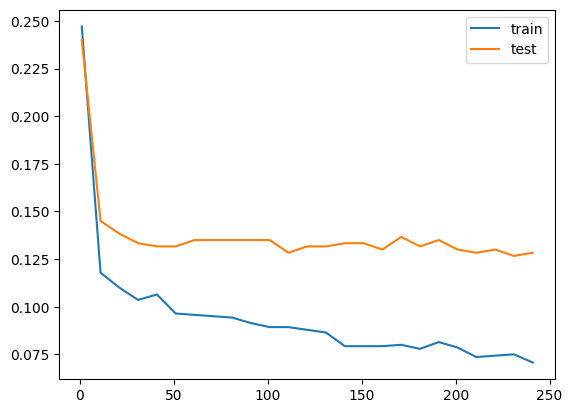
\includegraphics[width=0.8\textwidth]{../figures/2/output.png}
    \caption{Curva de erro de treinamento e teste a cada iteração}
\end{figure}

A figura acima demonstra a evolução do erro de treinamento e teste a cada iteração
do AdaBoost. O erro de treinamento diminui continuamente, apesar de demonstrar
pequenos aumentos em alguns pontos, o que é esperado dado o processo de reamostragem. Já o
erro de teste inicialmente diminui, atingindo um plateau, que se mantem até o final
do processo. Ao contrário do Random Forest ou Bagging, o AdaBoost pode
apresentar overfitting, de modo que, caso aumentemos o número de iterações, é
possível que o erro de teste comece a aumentar, enquanto o erro de treinamento
continuará a diminuir.

\newpage

\section*{Exercício 3}
\addcontentsline{toc}{section}{Exercício 3}

\subsection*{Exercício 3a}
\addcontentsline{toc}{subsection}{Exercício 3a}
\subsection*{Exercício 3}
\addcontentsline{toc}{subsection}{Exercício 3}

Este exercício utiliza o dataset MNIST para comparar diferentes algoritmos de classificação de dígitos manuscritos.

\subsubsection*{Configuração inicial e carregamento dos dados}

\begin{lstlisting}[language=Python]
from sklearn.datasets import fetch_openml
from sklearn.neighbors import KNeighborsClassifier
from sklearn.naive_bayes import BernoulliNB
from sklearn.discriminant_analysis import LinearDiscriminantAnalysis
from sklearn.discriminant_analysis import QuadraticDiscriminantAnalysis
from sklearn.linear_model import LogisticRegression
from sklearn.ensemble import RandomForestClassifier
from sklearn.neural_network import MLPClassifier
from sklearn.metrics import confusion_matrix
from sklearn import svm
from sklearn.model_selection import train_test_split
import numpy as np
import matplotlib.pyplot as plt

def plot_digits(
    images,
    n_rows=2,
    n_cols=5,
    fig_shape=(20, 8),
    indexes=[0, 1, 2, 3, 4, 5, 6, 7, 8, 9],
    img_shape=(28, 28),
    labels=[0, 1, 2, 3, 4, 5, 6, 7, 8, 9],
):
    fig, axs = plt.subplots(n_rows, n_cols, figsize=fig_shape)
    ind = np.array(indexes).reshape(n_rows, n_cols)
    if labels:
        plt_labels = np.array(labels).reshape(n_rows, n_cols)
    for i in range(0, n_rows):
        for j in range(0, n_cols):
            if labels:
                axs[i, j].set_title(plt_labels[i, j], fontsize=20)
            axs[i, j].imshow(
                (images[ind[i, j]].reshape(img_shape)), cmap="plasma"
            )
            axs[i, j].axis("off")

mnist = fetch_openml("mnist_784")  # Baixar os dados
X, y = mnist.data.to_numpy(), mnist.target.to_numpy()
X = X / 255  # Colocar as features em [0, 1]
# Divisão em treino e teste
X_train, X_test, y_train, y_test = train_test_split(
    X, y, test_size=0.2, random_state=42
)
# Plot dos dígitos
plot_digits(
    X, n_rows=2, n_cols=5, indexes=[21, 24, 16, 27, 26, 35, 13, 15, 17, 19]
)
\end{lstlisting}

\begin{figure}[H]
    \centering
    \includegraphics[width=0.8\textwidth]{../figures/3/mnist_samples.png}
    \caption{Exemplos de dígitos do dataset MNIST}
    \label{fig:mnist_samples}
\end{figure}

\subsubsection*{(a) Comparação de modelos: acurácia e tempo de execução}

\begin{lstlisting}[language=Python]
from sklearn.metrics import accuracy_score
import time

nb = BernoulliNB(force_alpha=True)  # Naive Bayes com features bernoulli
lda = LinearDiscriminantAnalysis()  # LDA
qda = QuadraticDiscriminantAnalysis(reg_param=0.01)  # QDA
lr = LogisticRegression(random_state=42)  # Regressão Logística
knn = KNeighborsClassifier(n_neighbors=6)  # kNN com k = 6
svc = svm.SVC(gamma="scale", class_weight="balanced", C=100)  # SVM
rf = RandomForestClassifier(
    max_depth=30, random_state=0, n_estimators=100
)  # Random forest
nn = MLPClassifier(
    random_state=42, hidden_layer_sizes=[100], max_iter=300
)  # Rede neural

models = [nb, lda, qda, lr, knn, svc, rf, nn]

yhats = []
accuracy = []
time_train = []
time_test = []
i = 0
for model in models:
    start_time = time.time()
    model.fit(X_train, y_train)
    end_time = time.time()
    time_train.append(end_time - start_time)

    start_time = time.time()
    yhat = model.predict(X_test)
    end_time = time.time()
    time_test.append(end_time - start_time)

    yhats.append(yhat)
    accuracy.append(accuracy_score(y_true=y_test, y_pred=yhat))
    i += 1
\end{lstlisting}

\textbf{Resultados de acurácia e tempo de execução:}

\begin{table}[H]
    \centering
    \begin{tabular}{|l|c|c|c|}
        \hline
        \textbf{Modelo}     & \textbf{Acurácia} & \textbf{Tempo Treino (s)} & \textbf{Tempo Teste (s)} \\
        \hline
        Naive Bayes         & [ACURACIA\_NB]    & [TEMPO\_TREINO\_NB]       & [TEMPO\_TESTE\_NB]       \\
        LDA                 & [ACURACIA\_LDA]   & [TEMPO\_TREINO\_LDA]      & [TEMPO\_TESTE\_LDA]      \\
        QDA                 & [ACURACIA\_QDA]   & [TEMPO\_TREINO\_QDA]      & [TEMPO\_TESTE\_QDA]      \\
        Regressão Logística & [ACURACIA\_LR]    & [TEMPO\_TREINO\_LR]       & [TEMPO\_TESTE\_LR]       \\
        kNN                 & [ACURACIA\_KNN]   & [TEMPO\_TREINO\_KNN]      & [TEMPO\_TESTE\_KNN]      \\
        SVM                 & [ACURACIA\_SVM]   & [TEMPO\_TREINO\_SVM]      & [TEMPO\_TESTE\_SVM]      \\
        Random Forest       & [ACURACIA\_RF]    & [TEMPO\_TREINO\_RF]       & [TEMPO\_TESTE\_RF]       \\
        Rede Neural         & [ACURACIA\_NN]    & [TEMPO\_TREINO\_NN]       & [TEMPO\_TESTE\_NN]       \\
        \hline
    \end{tabular}
    \caption{Comparação de acurácia e tempos de execução dos modelos}
    \label{tab:model_comparison}
\end{table}

\textbf{Observações:}
\begin{itemize}
    \item Para a convergência do modelo de QDA, foi necessário adicionar um parâmetro de regularização \texttt{reg\_param = 0.01}.
    \item Os dados não foram normalizados, dada a escala semelhante das features.
\end{itemize}

\subsubsection*{(b) Análise da interpretabilidade dos modelos}

Para cada um dos gráficos gerados pelos códigos abaixo, explicamos o que está sendo mostrado, como isso se relaciona com as previsões do modelo em questão e se é possível interpretar com facilidade o que está acontecendo.

\textbf{(i) Parâmetros do Naive Bayes}

\begin{lstlisting}[language=Python]
nb_params = {}
for i in range(10):
    nb_params[i] = np.exp(nb.feature_log_prob_[i])

plot_digits(nb_params)
\end{lstlisting}

\begin{figure}[H]
    \centering
    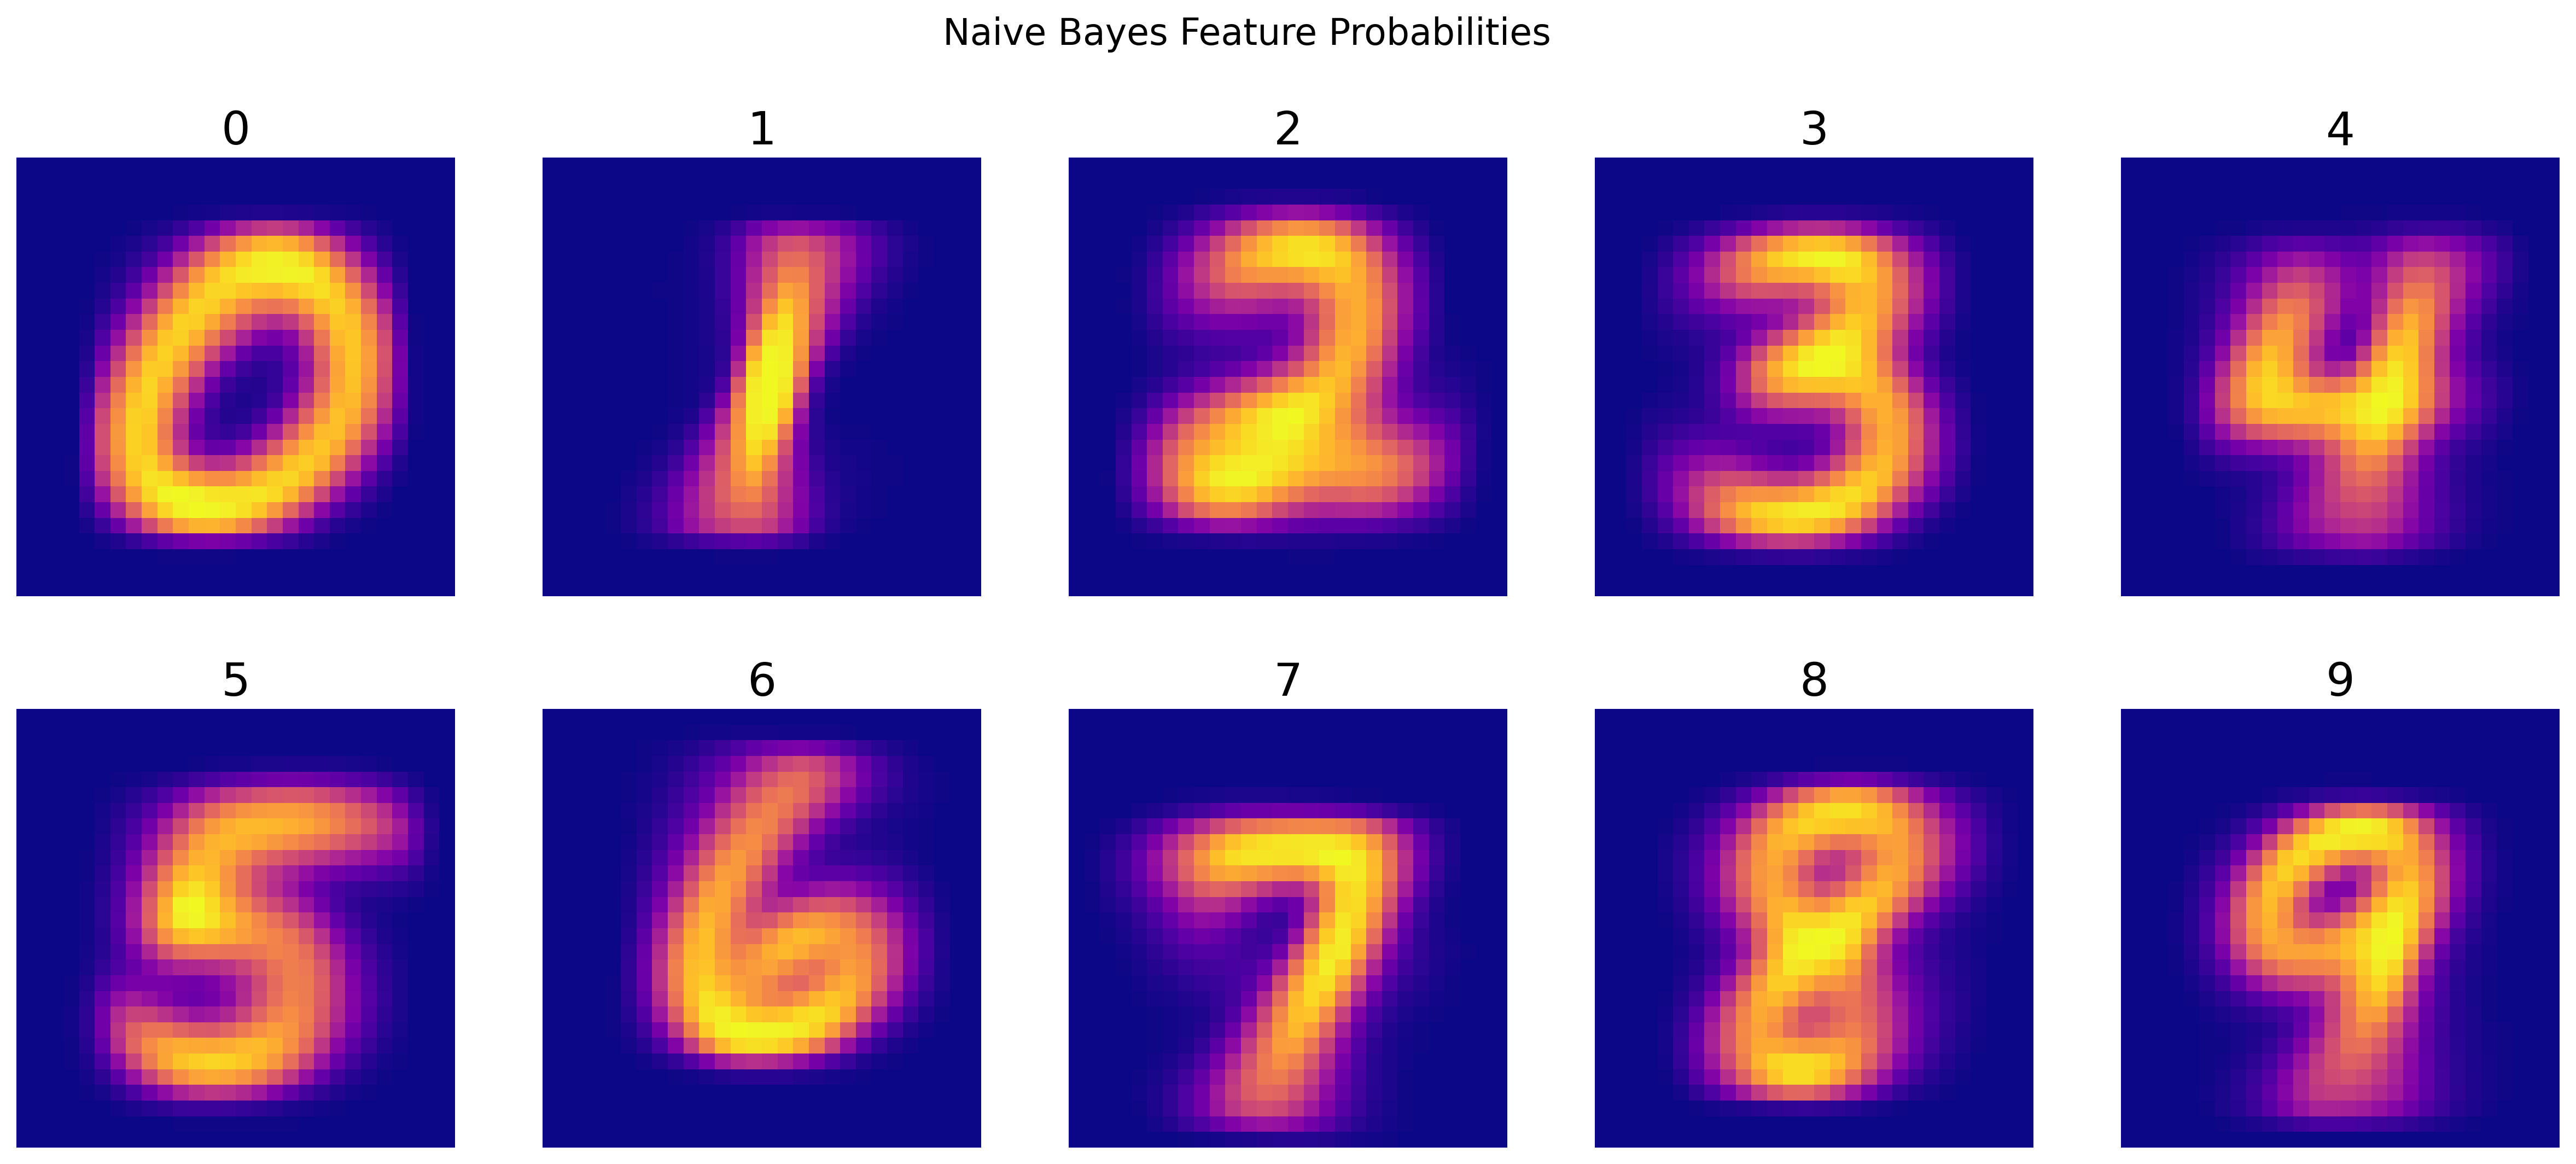
\includegraphics[width=0.8\textwidth]{../figures/3/naive_bayes_params.png}
    \caption{Probabilidades dos pixels para cada classe no modelo Naive Bayes}
    \label{fig:nb_params}
\end{figure}

Cada imagem representa a probabilidade dos pixels da imagem pertencerem à respectiva classe, sendo que valores altos indicam pixels recorrentes para a classe. O produto entre este vetor e a entrada indicará a probabilidade da entrada ser pertencente à classe e será utilizada para classificação. A interpretação da imagem é simples e permite a reconstituição do dígito ao qual a classe referencia.

\textbf{(ii) Parâmetros do LDA}

\begin{lstlisting}[language=Python]
lda_params = {}
for i in range(10):
    lda_params[i] = lda.means_[i]

plot_digits(lda_params)
\end{lstlisting}

\begin{figure}[H]
    \centering
    \includegraphics[width=0.8\textwidth]{../figures/3/lda_means.png}
    \caption{Médias das classes no modelo LDA}
    \label{fig:lda_means}
\end{figure}

Cada uma das imagens é a média da respectiva classe no espaço de entrada. Essa imagem seria equivalente a uma amostra média, ponto central em relação às demais amostras da classe. As previsões do modelo baseiam-se em uma métrica de similaridade da entrada em relação a cada uma dessas médias. É possível interpretar com facilidade a classe relacionada a cada imagem.

\textbf{(iii) Parâmetros da Regressão Logística}

\begin{lstlisting}[language=Python]
log_reg_params = {}
for i in range(10):
    log_reg_params[i] = lr.coef_[i]

plot_digits(log_reg_params)
\end{lstlisting}

\begin{figure}[H]
    \centering
    \includegraphics[width=0.8\textwidth]{../figures/3/logistic_regression_coefs.png}
    \caption{Coeficientes do modelo de Regressão Logística}
    \label{fig:lr_coefs}
\end{figure}

A imagem representa o coeficiente da rede. Ao multiplicarmos pela entrada, teremos o logaritmo da probabilidade da amostra pertencer à classe sobre a probabilidade dela pertencer à classe de referência. A imagem mostrada é a resposta do modelo a uma matriz de 1's. Isso pode ser interpretado como a contribuição de cada pixel para a probabilidade final. Ainda mantemos uma interpretação válida de cada classe por meio da imagem, apesar de menos clara caso comparemos com as imagens dos modelos anteriores.

\textbf{(iv) Importância das features no Random Forest}

\begin{lstlisting}[language=Python]
rf_params = rf.feature_importances_.reshape(28, 28)

plt.axis("off")
plt.imshow(rf_params, cmap="plasma")
\end{lstlisting}

\begin{figure}[H]
    \centering
    \includegraphics[width=0.6\textwidth]{../figures/3/random_forest_importance.png}
    \caption{Importância das features no modelo Random Forest}
    \label{fig:rf_importance}
\end{figure}

A imagem representa a importância de cada pixel para o modelo, baseada na média do decaimento de uma métrica de impureza, no caso, o coeficiente de Gini. Valores altos indicam que aquela feature foi capaz de auxiliar na distinção entre as classes. Nesse caso, perde-se a interpretação individual das classes, entretanto ainda está clara qual a região mais importante para a classificação.

\textbf{(v) Parâmetros da Rede Neural}

\textbf{(v.a) Pesos da camada de entrada para a camada oculta}

\begin{lstlisting}[language=Python]
nn_params_1 = {}
for i in range(100):
    nn_params_1[i] = nn.coefs_[0][:, i]

indexes = list(range(100))

plot_digits(
    nn_params_1,
    n_rows=10,
    n_cols=10,
    fig_shape=(100, 100),
    indexes=indexes,
    img_shape=(28, 28),
    labels=None,
)
\end{lstlisting}

\begin{figure}[H]
    \centering
    \includegraphics[width=0.9\textwidth]{../figures/3/neural_network_layer1_weights.png}
    \caption{Pesos da camada de entrada para a camada oculta na Rede Neural}
    \label{fig:nn_layer1}
\end{figure}

Cada imagem representa os pesos que ligam a entrada a cada um dos neurônios da camada oculta. Eles são a transformação linear da entrada antes da primeira função de ativação e podem ser interpretados como parte de uma engenharia de features. A interpretabilidade já se perdeu completamente, tanto pela alta quantidade de neurônios quanto pela dificuldade de encontrar valor semântico em cada transformação.

\textbf{(v.b) Pesos da camada oculta para a camada de saída}

\begin{lstlisting}[language=Python]
nn_params_2 = {}
for i in range(10):
    nn_params_2[i] = nn.coefs_[1][:, i]

plot_digits(
    nn_params_2, n_rows=2, n_cols=5, fig_shape=(20, 8), img_shape=(10, 10)
)
\end{lstlisting}

\begin{figure}[H]
    \centering
    \includegraphics[width=0.8\textwidth]{../figures/3/neural_network_layer2_weights.png}
    \caption{Pesos da camada oculta para a camada de saída na Rede Neural}
    \label{fig:nn_layer2}
\end{figure}

Cada imagem representa os pesos que ligam a camada escondida da rede à camada de saída, em que uma regressão logística será realizada. Seria semelhante ao que ocorre no modelo de regressão logística do item anterior. Entretanto, como o espaço de features é a projeção da entrada na camada intermediária, a interpretação se perde, não podendo relacionar cada classe ao numeral correspondente.

\subsubsection*{(c) Análise da matriz de confusão do Naive Bayes}

\begin{lstlisting}[language=Python]
cm = confusion_matrix(y_true=y_test, y_pred=yhats[0])
mask = 1 - np.identity(cm.shape[0])
error_matrix = np.multiply(cm, mask)

error_perc = error_matrix.sum(axis=1) / cm.sum(axis=1)

value, count = np.unique(y_train, return_counts=True)
\end{lstlisting}

\begin{figure}[H]
    \centering
    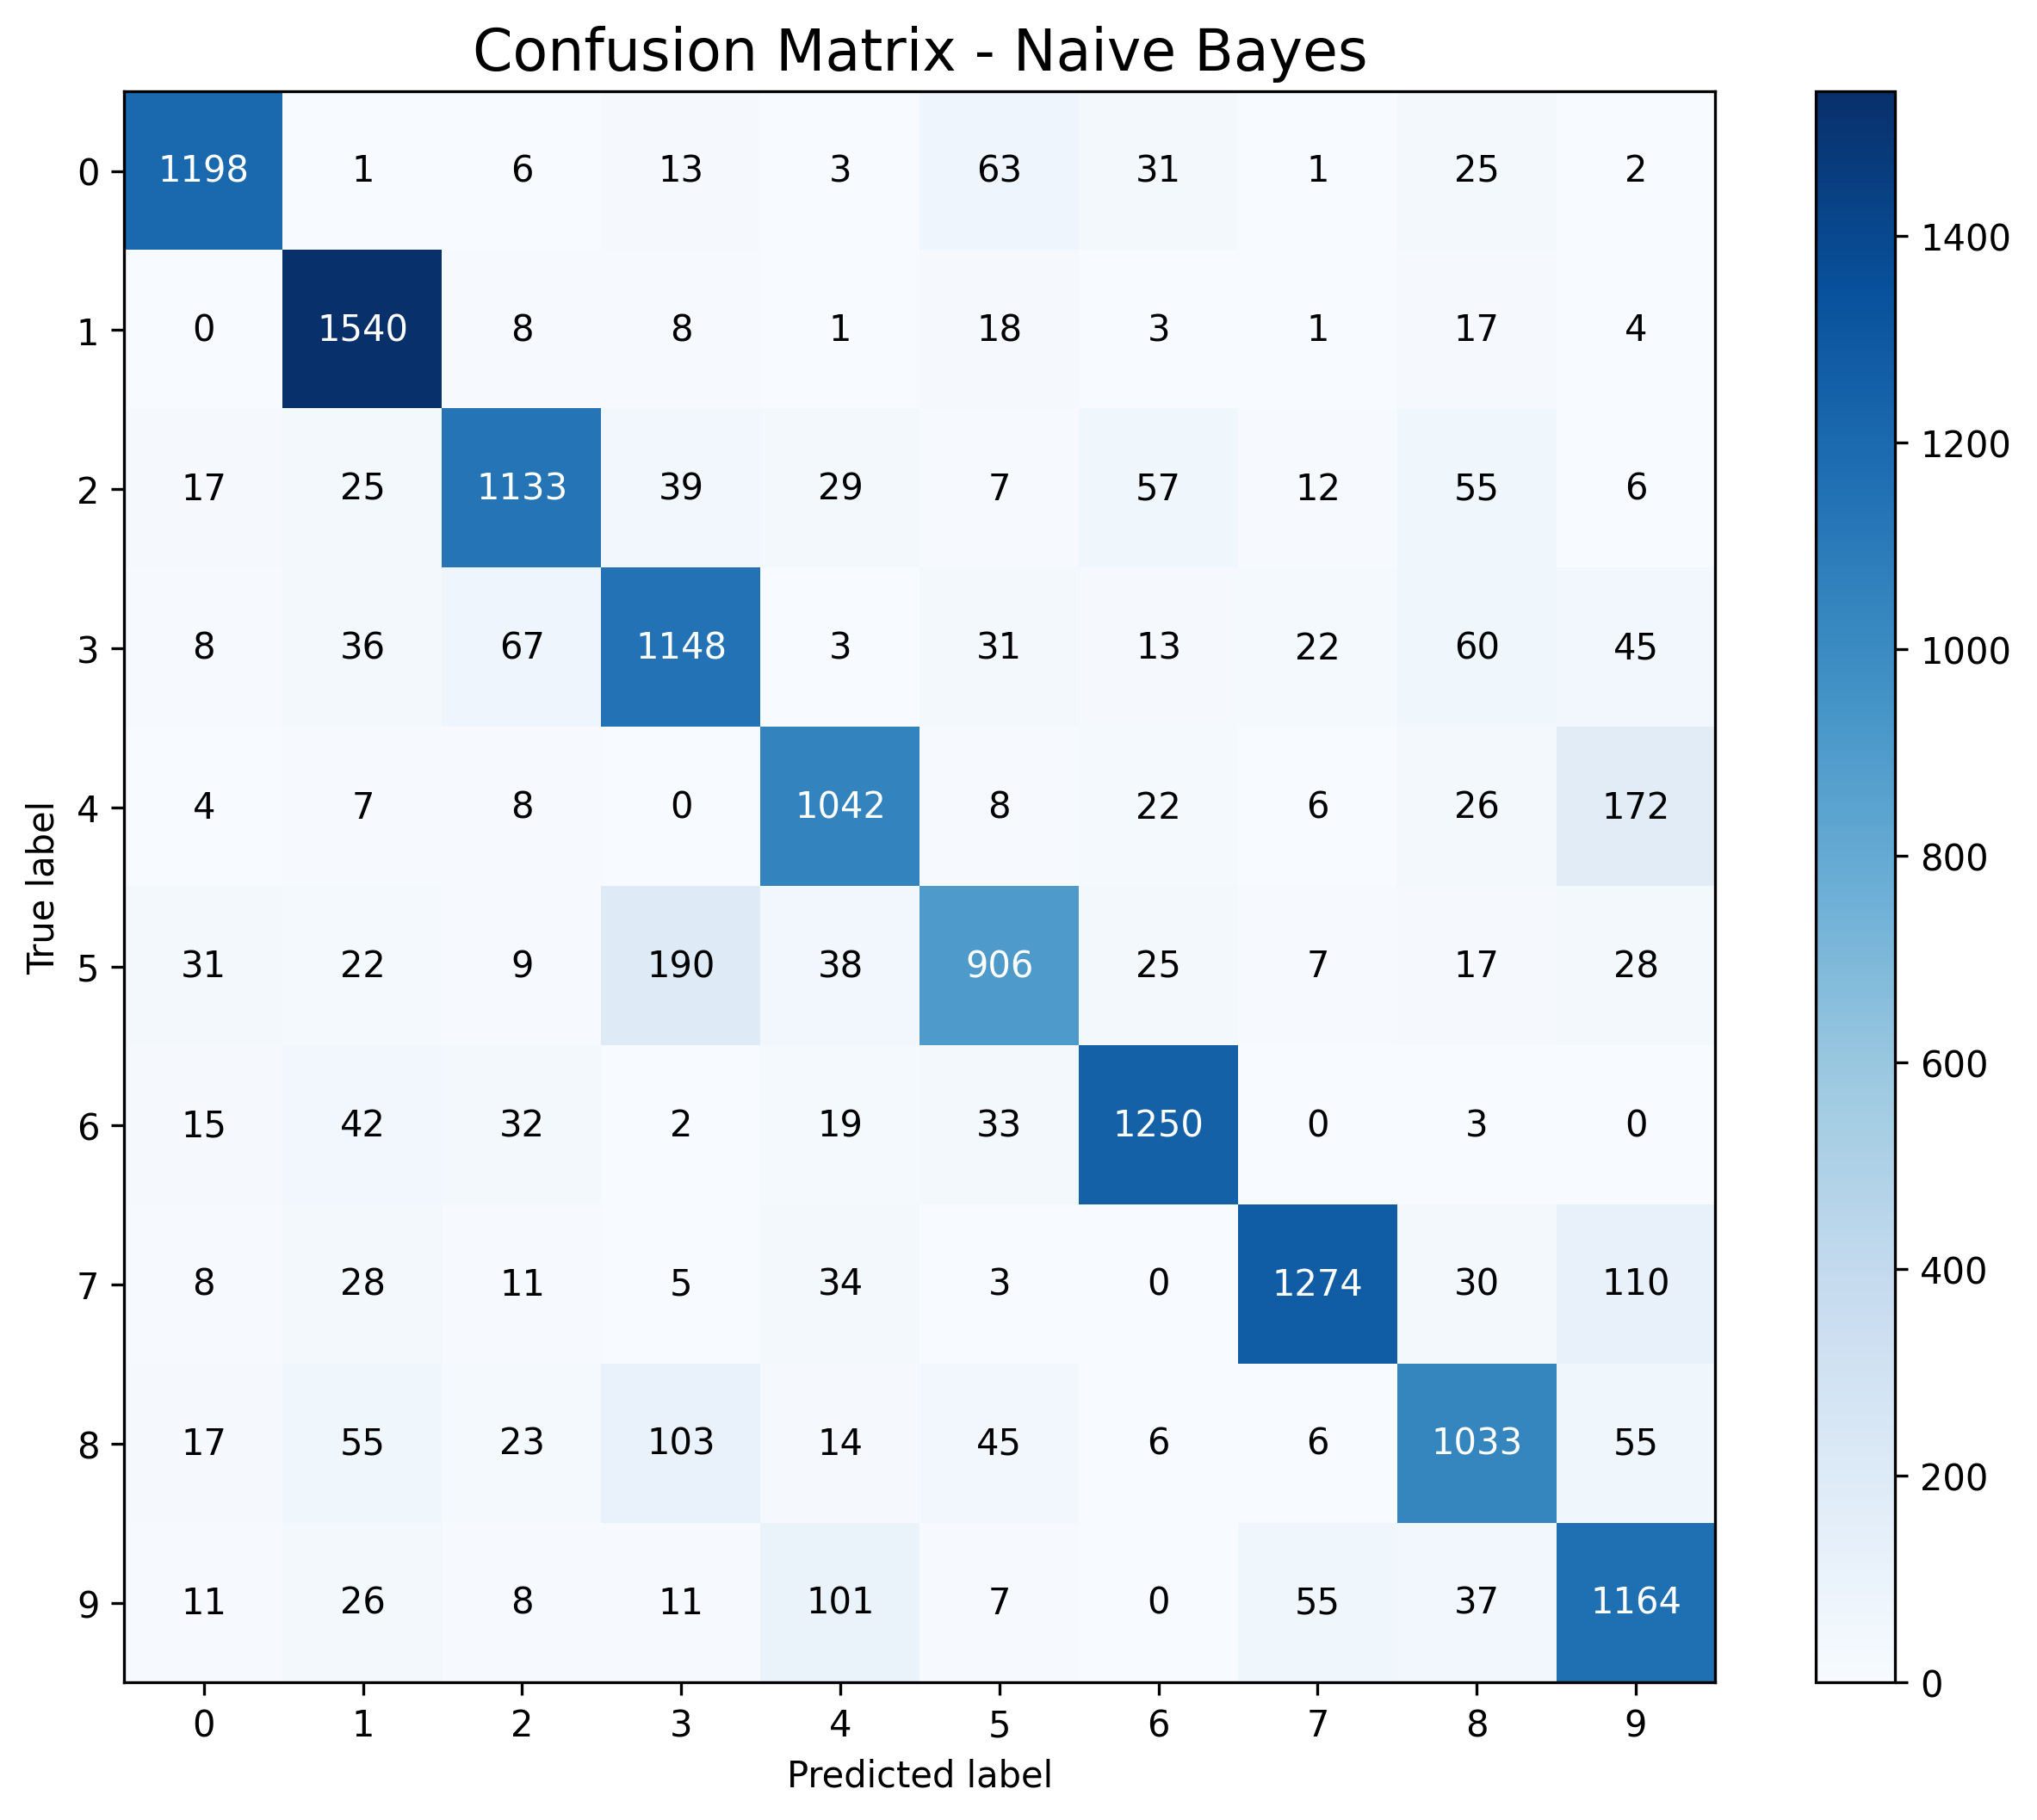
\includegraphics[width=0.8\textwidth]{../figures/3/confusion_matrix_naive_bayes.png}
    \caption{Matriz de confusão do modelo Naive Bayes}
    \label{fig:confusion_matrix}
\end{figure}

\textbf{Análise dos erros mais comuns:}

\begin{table}[H]
    \centering
    \begin{tabular}{|c|c|}
        \hline
        \textbf{Classe} & \textbf{Taxa de Erro (\%)} \\
        \hline
        0               & [ERRO\_CLASSE\_0]          \\
        1               & [ERRO\_CLASSE\_1]          \\
        2               & [ERRO\_CLASSE\_2]          \\
        3               & [ERRO\_CLASSE\_3]          \\
        4               & [ERRO\_CLASSE\_4]          \\
        5               & [ERRO\_CLASSE\_5]          \\
        6               & [ERRO\_CLASSE\_6]          \\
        7               & [ERRO\_CLASSE\_7]          \\
        8               & [ERRO\_CLASSE\_8]          \\
        9               & [ERRO\_CLASSE\_9]          \\
        \hline
    \end{tabular}
    \caption{Taxa de erro por classe no modelo Naive Bayes}
    \label{tab:error_rates}
\end{table}

A classe mais confundida foi a \textbf{[CLASSE\_MAIS\_ERRADA]}. Nota-se pela matriz de confusão que parte considerável dos erros para esta classe ocorreram pois o modelo previu [CLASSES\_CONFUNDIDAS]. Provavelmente isso acontece pela semelhança dos dígitos [DIGITOS\_SIMILARES] e pelo desbalanceamento da classe [CLASSE\_MAIS\_FREQUENTE] nos dados de treino, que foi a mais frequente.

\textbf{Contagem das classes nos dados de treino:}

\begin{table}[H]
    \centering
    \begin{tabular}{|c|c|c|c|c|c|c|c|c|c|c|}
        \hline
        \textbf{Classe}   & 0          & 1          & 2          & 3          & 4          & 5          & 6          & 7          & 8          & 9          \\
        \hline
        \textbf{Contagem} & [COUNT\_0] & [COUNT\_1] & [COUNT\_2] & [COUNT\_3] & [COUNT\_4] & [COUNT\_5] & [COUNT\_6] & [COUNT\_7] & [COUNT\_8] & [COUNT\_9] \\
        \hline
    \end{tabular}
    \caption{Distribuição das classes no conjunto de treinamento}
    \label{tab:class_distribution}
\end{table}
\newpage

\subsection*{Exercício 3b}
\addcontentsline{toc}{subsection}{Exercício 3b}
\subsubsection*{(b) Análise da interpretabilidade dos modelos}

Para cada um dos gráficos gerados pelos códigos abaixo, explicamos o que está sendo mostrado, como isso se relaciona com as previsões do modelo em questão e se é possível interpretar com facilidade o que está acontecendo.

\textbf{(i) Parâmetros do Naive Bayes}

\begin{lstlisting}[language=Python]
nb_params = {}
for i in range(10):
    nb_params[i] = np.exp(nb.feature_log_prob_[i])

plot_digits(nb_params)
\end{lstlisting}

\begin{figure}[H]
    \centering
    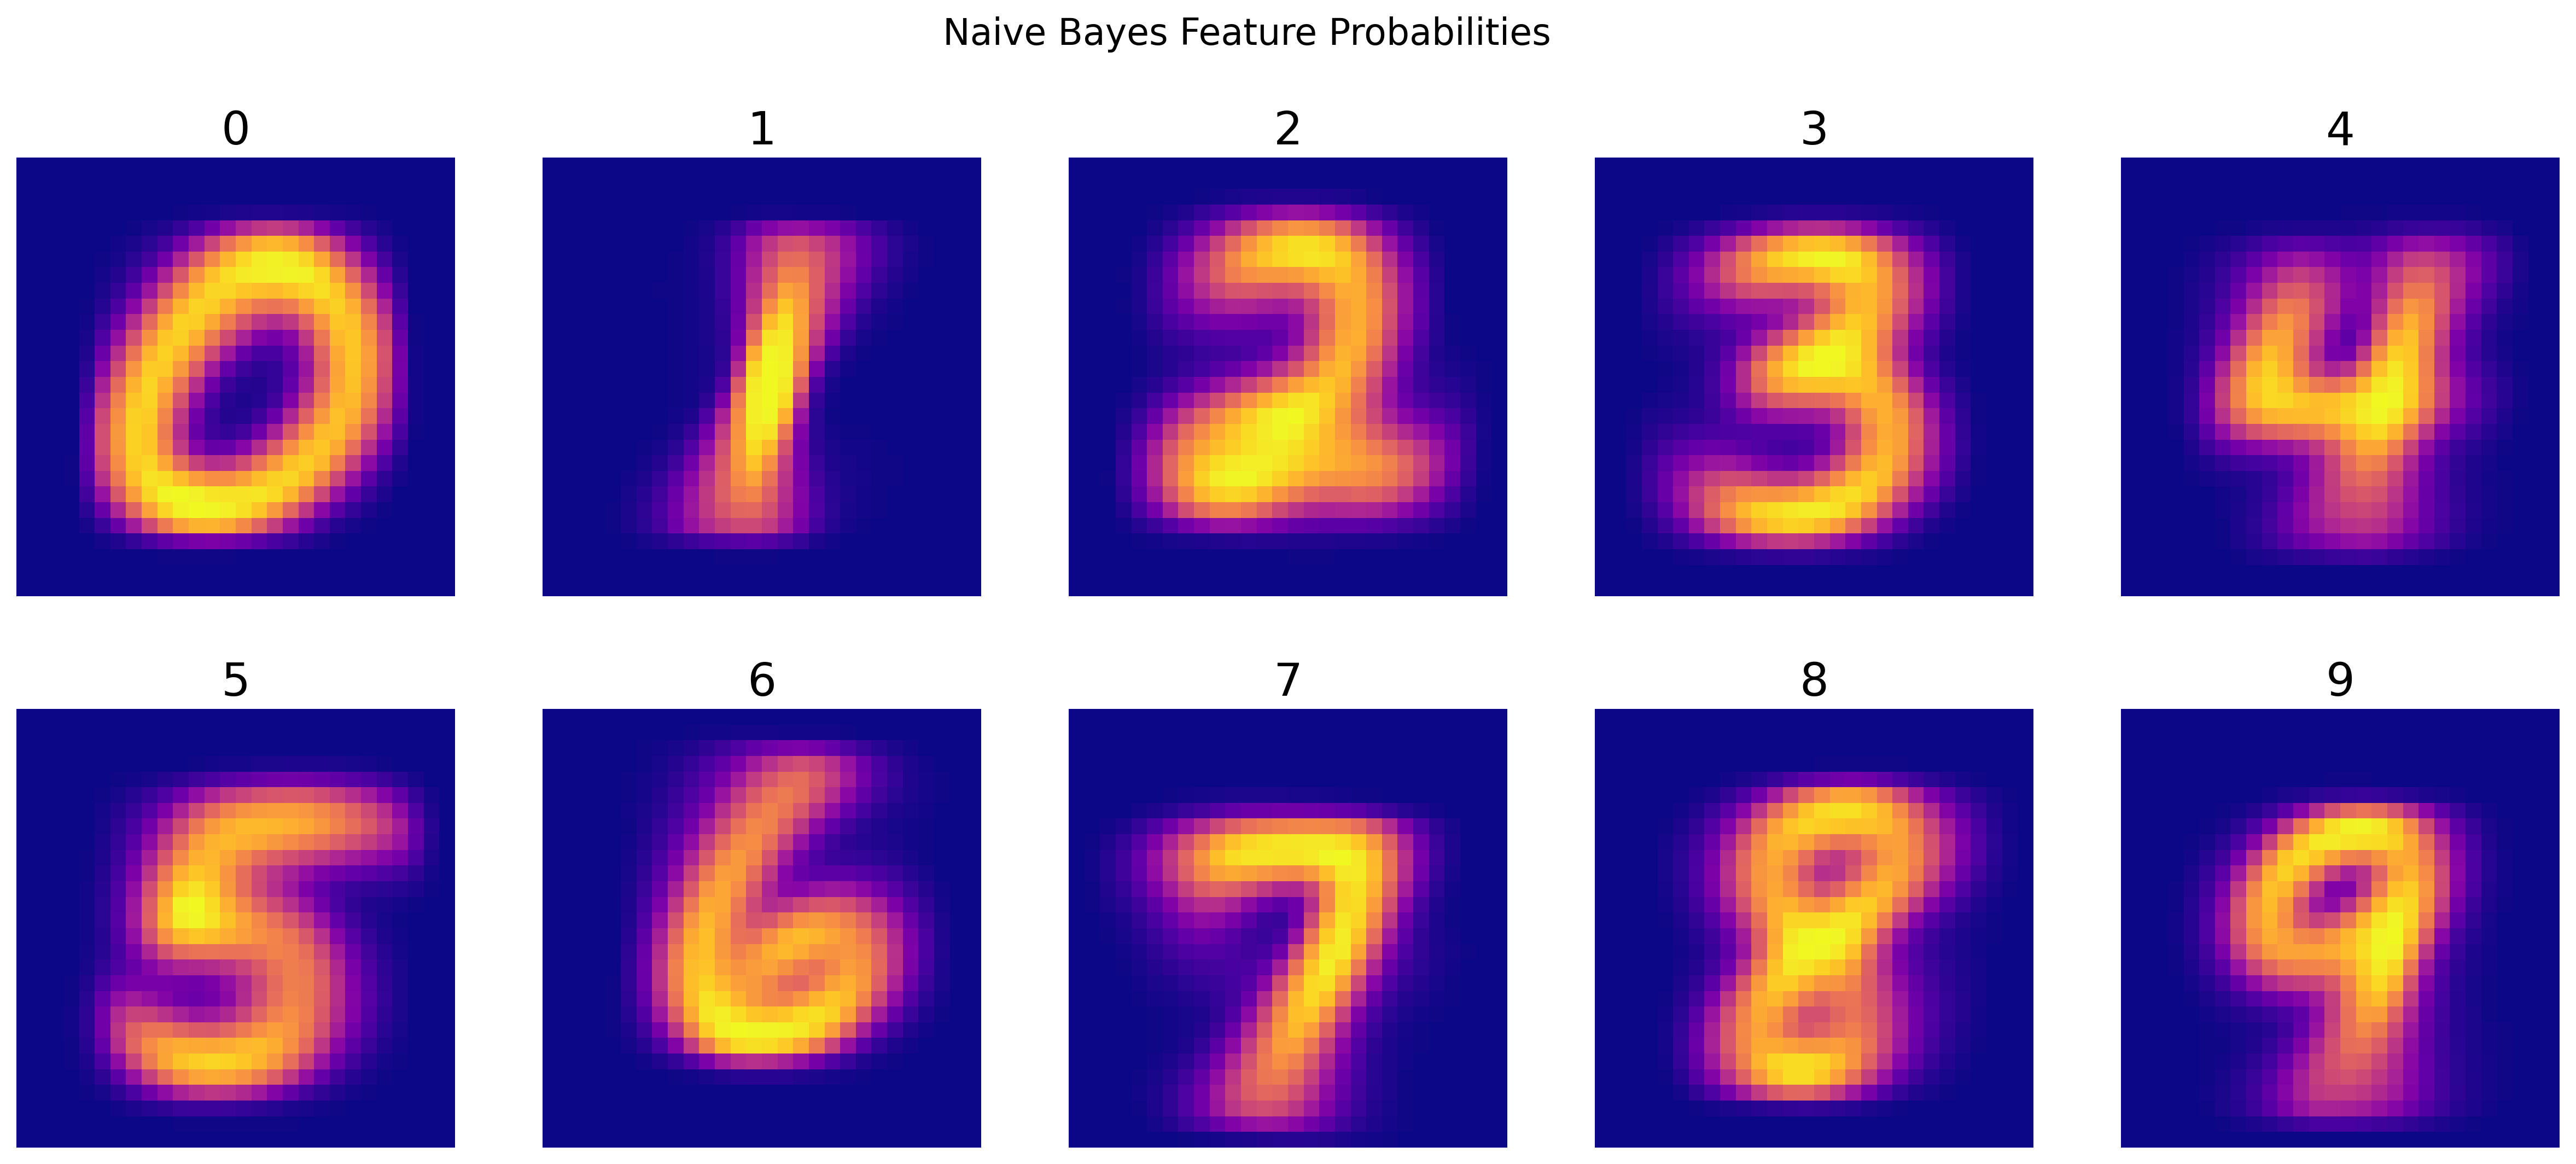
\includegraphics[width=0.8\textwidth]{../figures/3/naive_bayes_params.png}
    \caption{Probabilidades dos pixels para cada classe no modelo Naive Bayes}
    \label{fig:nb_params}
\end{figure}

Cada imagem representa a probabilidade dos pixels da imagem pertencerem à respectiva classe, sendo que valores altos indicam pixels recorrentes para a classe. O produto entre este vetor e a entrada indicará a probabilidade da entrada ser pertencente à classe e será utilizada para classificação. A interpretação da imagem é simples e permite a reconstituição do dígito ao qual a classe referencia.

\textbf{(ii) Parâmetros do LDA}

\begin{lstlisting}[language=Python]
lda_params = {}
for i in range(10):
    lda_params[i] = lda.means_[i]

plot_digits(lda_params)
\end{lstlisting}

\begin{figure}[H]
    \centering
    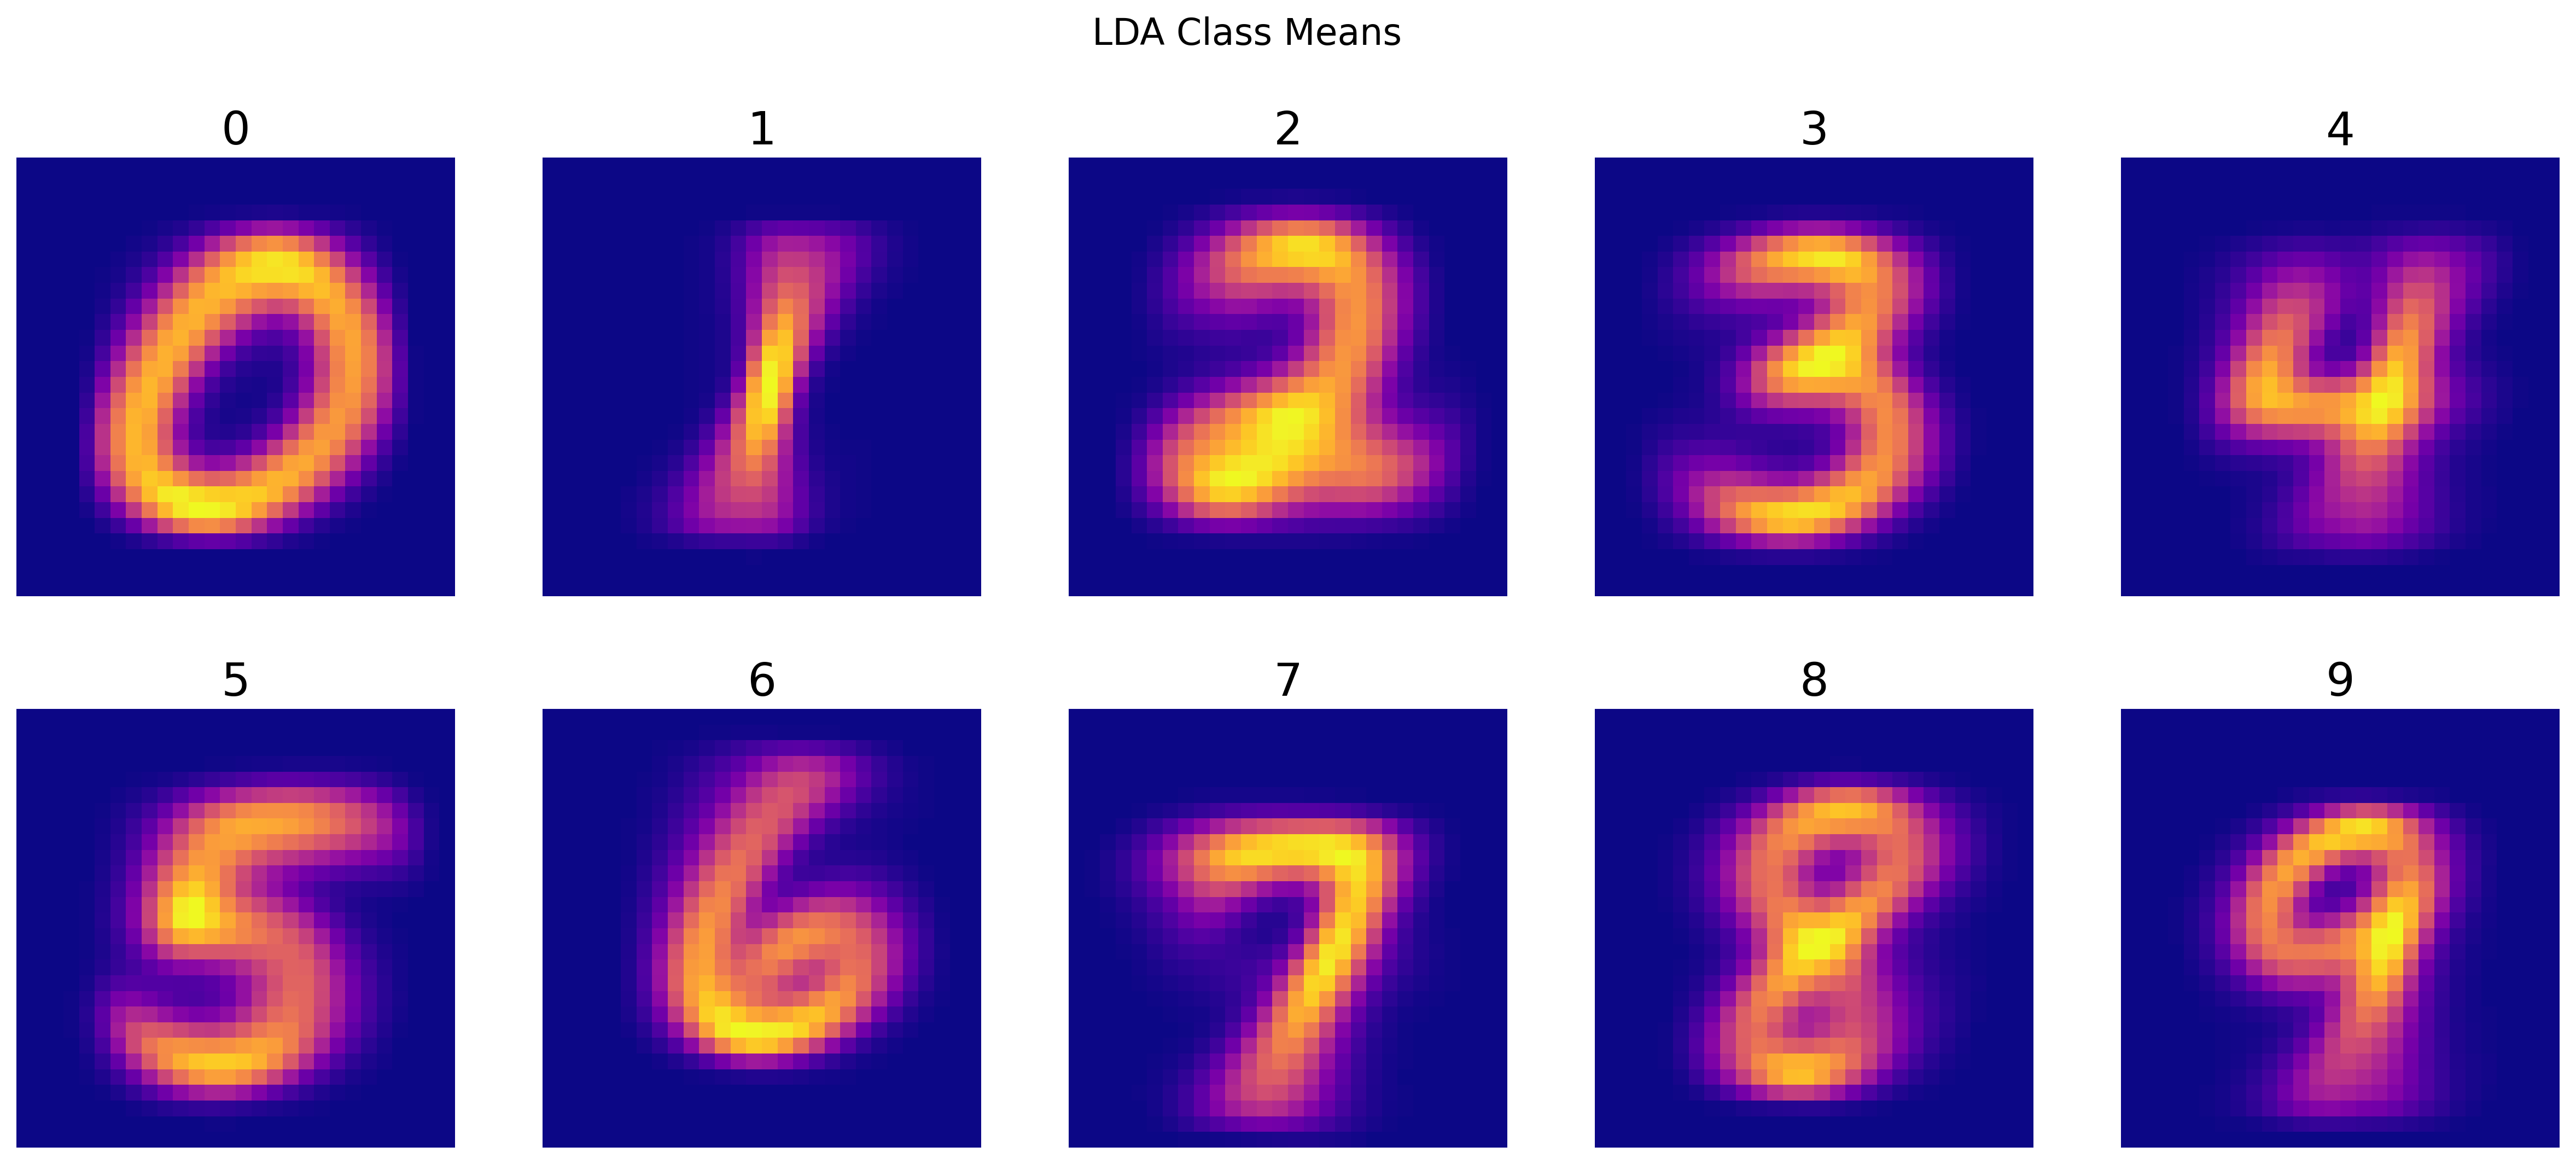
\includegraphics[width=0.8\textwidth]{../figures/3/lda_params.png}
    \caption{Médias das classes no modelo LDA}
    \label{fig:lda_means}
\end{figure}

Cada uma das imagens é a média da respectiva classe no espaço de entrada. Essa imagem seria equivalente a uma amostra média, ponto central em relação às demais amostras da classe. As previsões do modelo baseiam-se em uma métrica de similaridade da entrada em relação a cada uma dessas médias. É possível interpretar com facilidade a classe relacionada a cada imagem.

\textbf{(iii) Parâmetros da Regressão Logística}

\begin{lstlisting}[language=Python]
log_reg_params = {}
for i in range(10):
    log_reg_params[i] = lr.coef_[i]

plot_digits(log_reg_params)
\end{lstlisting}

\begin{figure}[H]
    \centering
    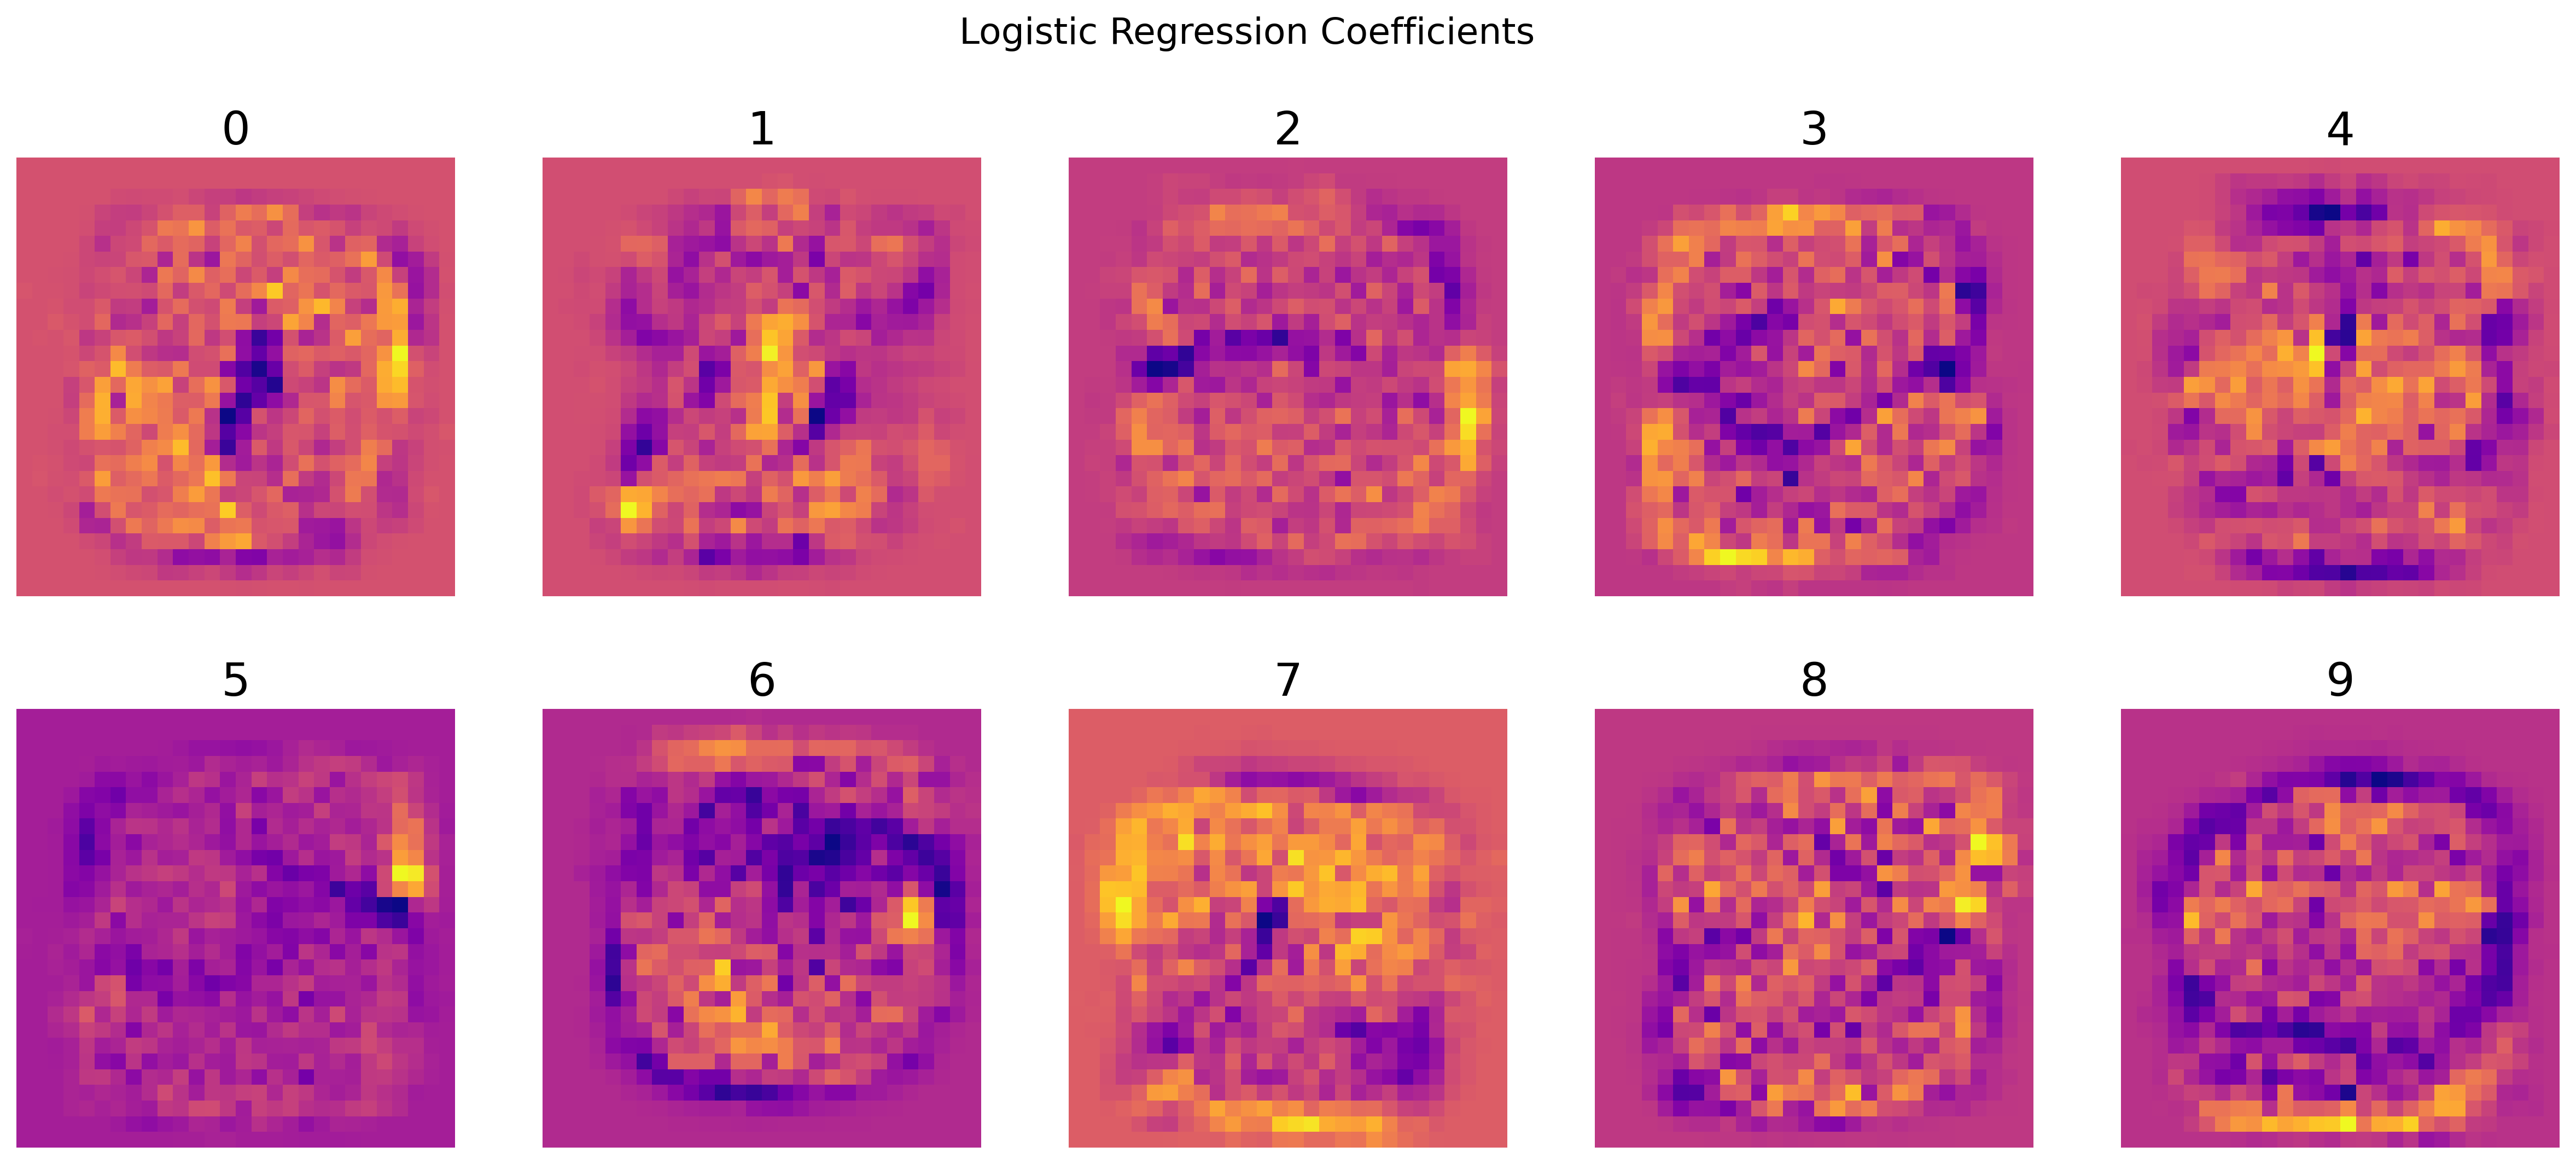
\includegraphics[width=0.8\textwidth]{../figures/3/logistic_regression_params.png}
    \caption{Coeficientes do modelo de Regressão Logística}
    \label{fig:lr_coefs}
\end{figure}

A imagem representa o coeficiente da rede. Ao multiplicarmos pela entrada, teremos o logaritmo da probabilidade da amostra pertencer à classe sobre a probabilidade dela pertencer à classe de referência. A imagem mostrada é a resposta do modelo a uma matriz de 1's. Isso pode ser interpretado como a contribuição de cada pixel para a probabilidade final. Ainda mantemos uma interpretação válida de cada classe por meio da imagem, apesar de menos clara caso comparemos com as imagens dos modelos anteriores.

\textbf{(iv) Importância das features no Random Forest}

\begin{lstlisting}[language=Python]
rf_params = rf.feature_importances_.reshape(28, 28)

plt.axis("off")
plt.imshow(rf_params, cmap="plasma")
\end{lstlisting}

\begin{figure}[H]
    \centering
    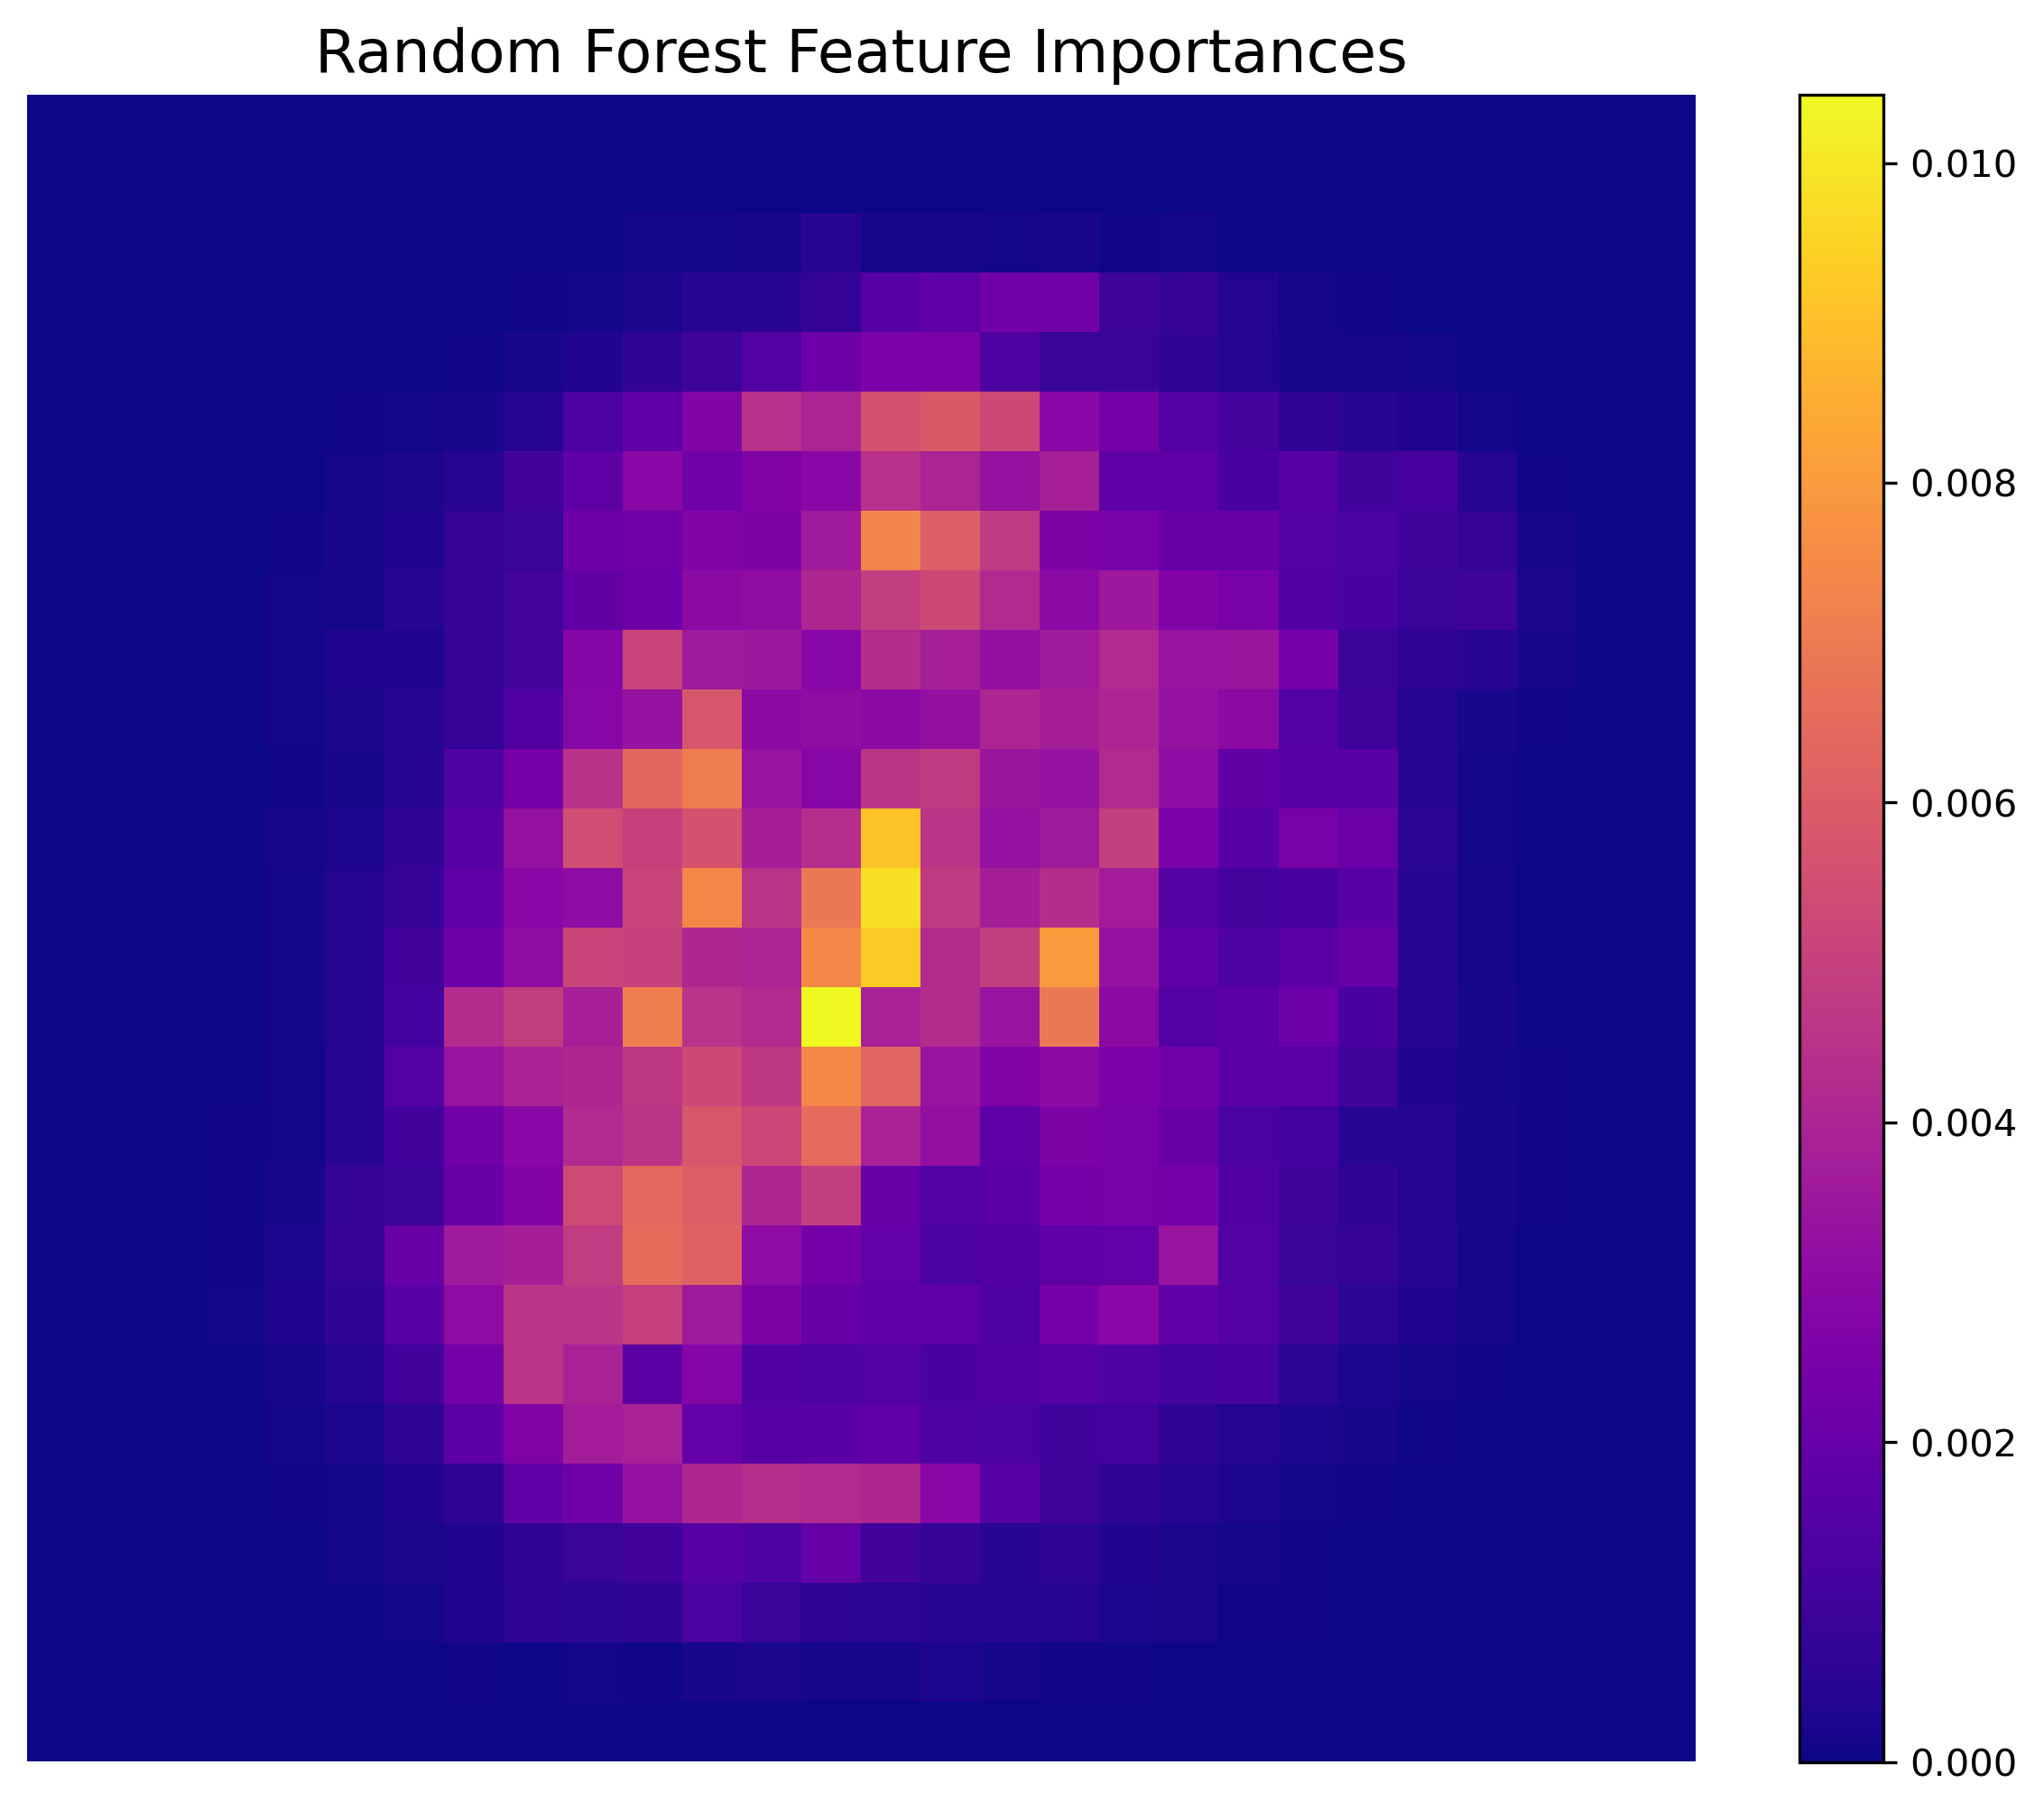
\includegraphics[width=0.6\textwidth]{../figures/3/random_forest_feature_importance.png}
    \caption{Importância das features no modelo Random Forest}
    \label{fig:rf_importance}
\end{figure}

A imagem representa a importância de cada pixel para o modelo, baseada na média do decaimento de uma métrica de impureza, no caso, o coeficiente de Gini. Valores altos indicam que aquela feature foi capaz de auxiliar na distinção entre as classes. Nesse caso, perde-se a interpretação individual das classes, entretanto ainda está clara qual a região mais importante para a classificação.

\textbf{(v) Parâmetros da Rede Neural}

\textbf{(v.a) Pesos da camada de entrada para a camada oculta}

\begin{lstlisting}[language=Python]
nn_params_1 = {}
for i in range(100):
    nn_params_1[i] = nn.coefs_[0][:, i]

indexes = list(range(100))

plot_digits(
    nn_params_1,
    n_rows=10,
    n_cols=10,
    fig_shape=(100, 100),
    indexes=indexes,
    img_shape=(28, 28),
    labels=None,
)
\end{lstlisting}

\begin{figure}[H]
    \centering
    \includegraphics[width=0.9\textwidth]{../figures/3/neural_network_input_hidden_weights.png}
    \caption{Pesos da camada de entrada para a camada oculta na Rede Neural}
    \label{fig:nn_layer1}
\end{figure}

Cada imagem representa os pesos que ligam a entrada a cada um dos neurônios da camada oculta. Eles são a transformação linear da entrada antes da primeira função de ativação e podem ser interpretados como parte de uma engenharia de features. A interpretabilidade já se perdeu completamente, tanto pela alta quantidade de neurônios quanto pela dificuldade de encontrar valor semântico em cada transformação.

\textbf{(v.b) Pesos da camada oculta para a camada de saída}

\begin{lstlisting}[language=Python]
nn_params_2 = {}
for i in range(10):
    nn_params_2[i] = nn.coefs_[1][:, i]

plot_digits(
    nn_params_2, n_rows=2, n_cols=5, fig_shape=(20, 8), img_shape=(10, 10)
)
\end{lstlisting}

\begin{figure}[H]
    \centering
    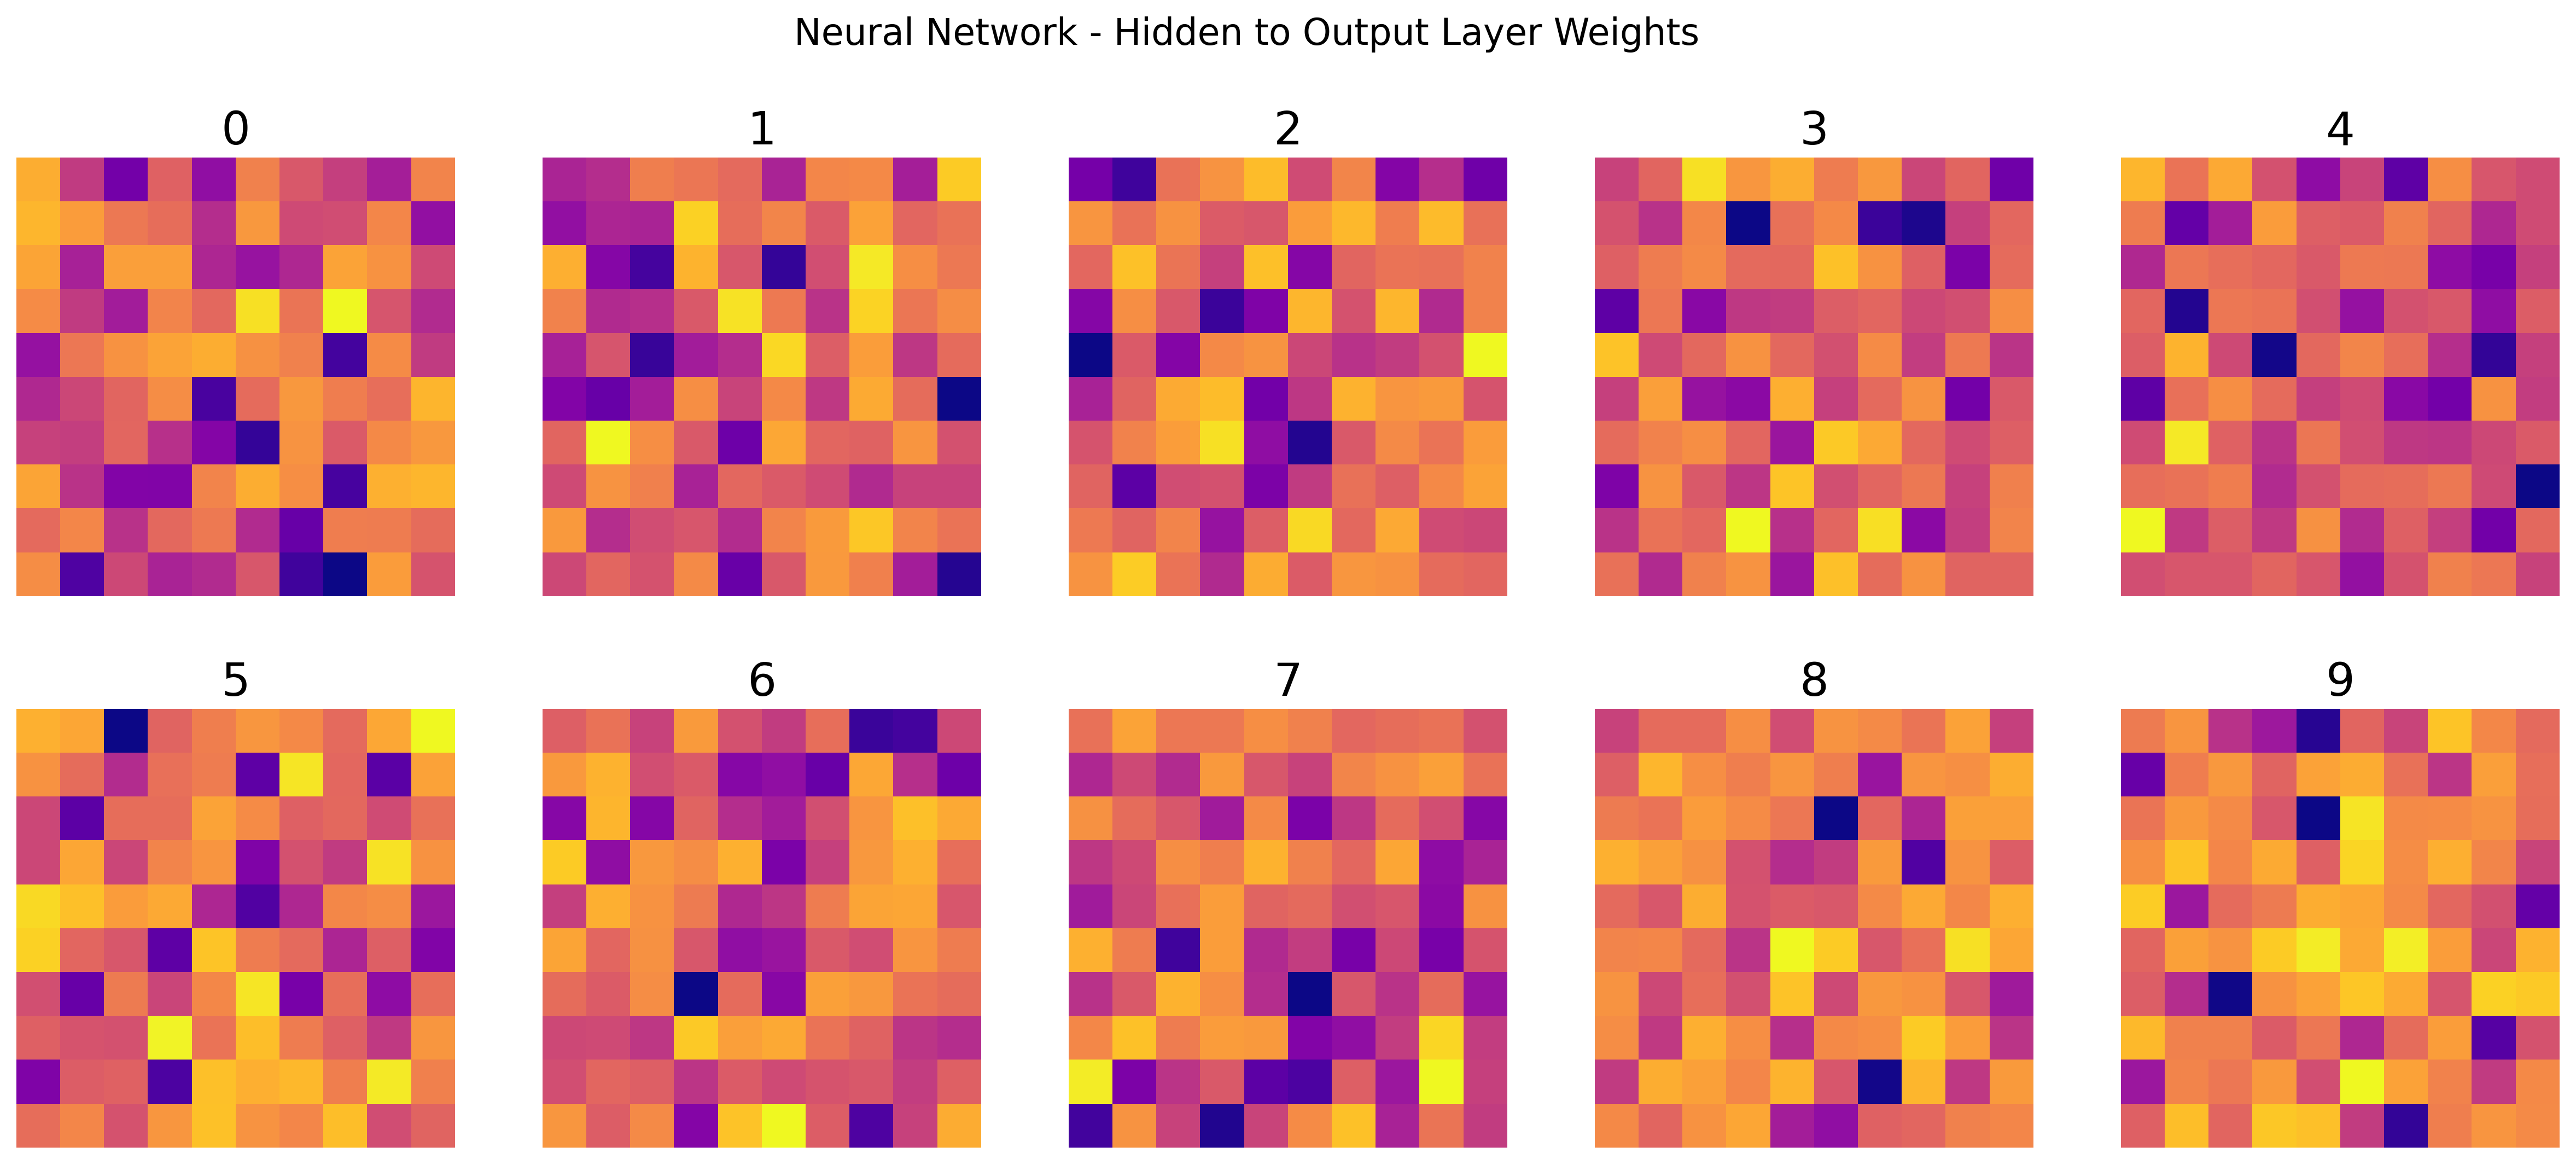
\includegraphics[width=0.8\textwidth]{../figures/3/neural_network_hidden_output_weights.png}
    \caption{Pesos da camada oculta para a camada de saída na Rede Neural}
    \label{fig:nn_layer2}
\end{figure}

Cada imagem representa os pesos que ligam a camada escondida da rede à camada de saída, em que uma regressão logística será realizada. Seria semelhante ao que ocorre no modelo de regressão logística do item anterior. Entretanto, como o espaço de features é a projeção da entrada na camada intermediária, a interpretação se perde, não podendo relacionar cada classe ao numeral correspondente.


\newpage

\subsection*{Exercício 3c}
\addcontentsline{toc}{subsection}{Exercício 3c}
\subsubsection*{(c) Análise da matriz de confusão do Naive Bayes}

\begin{lstlisting}[language=Python]
cm = confusion_matrix(y_true=y_test, y_pred=yhats[0])
mask = 1 - np.identity(cm.shape[0])
error_matrix = np.multiply(cm, mask)

error_perc = error_matrix.sum(axis=1) / cm.sum(axis=1)

value, count = np.unique(y_train, return_counts=True)
\end{lstlisting}

\begin{figure}[H]
    \centering
    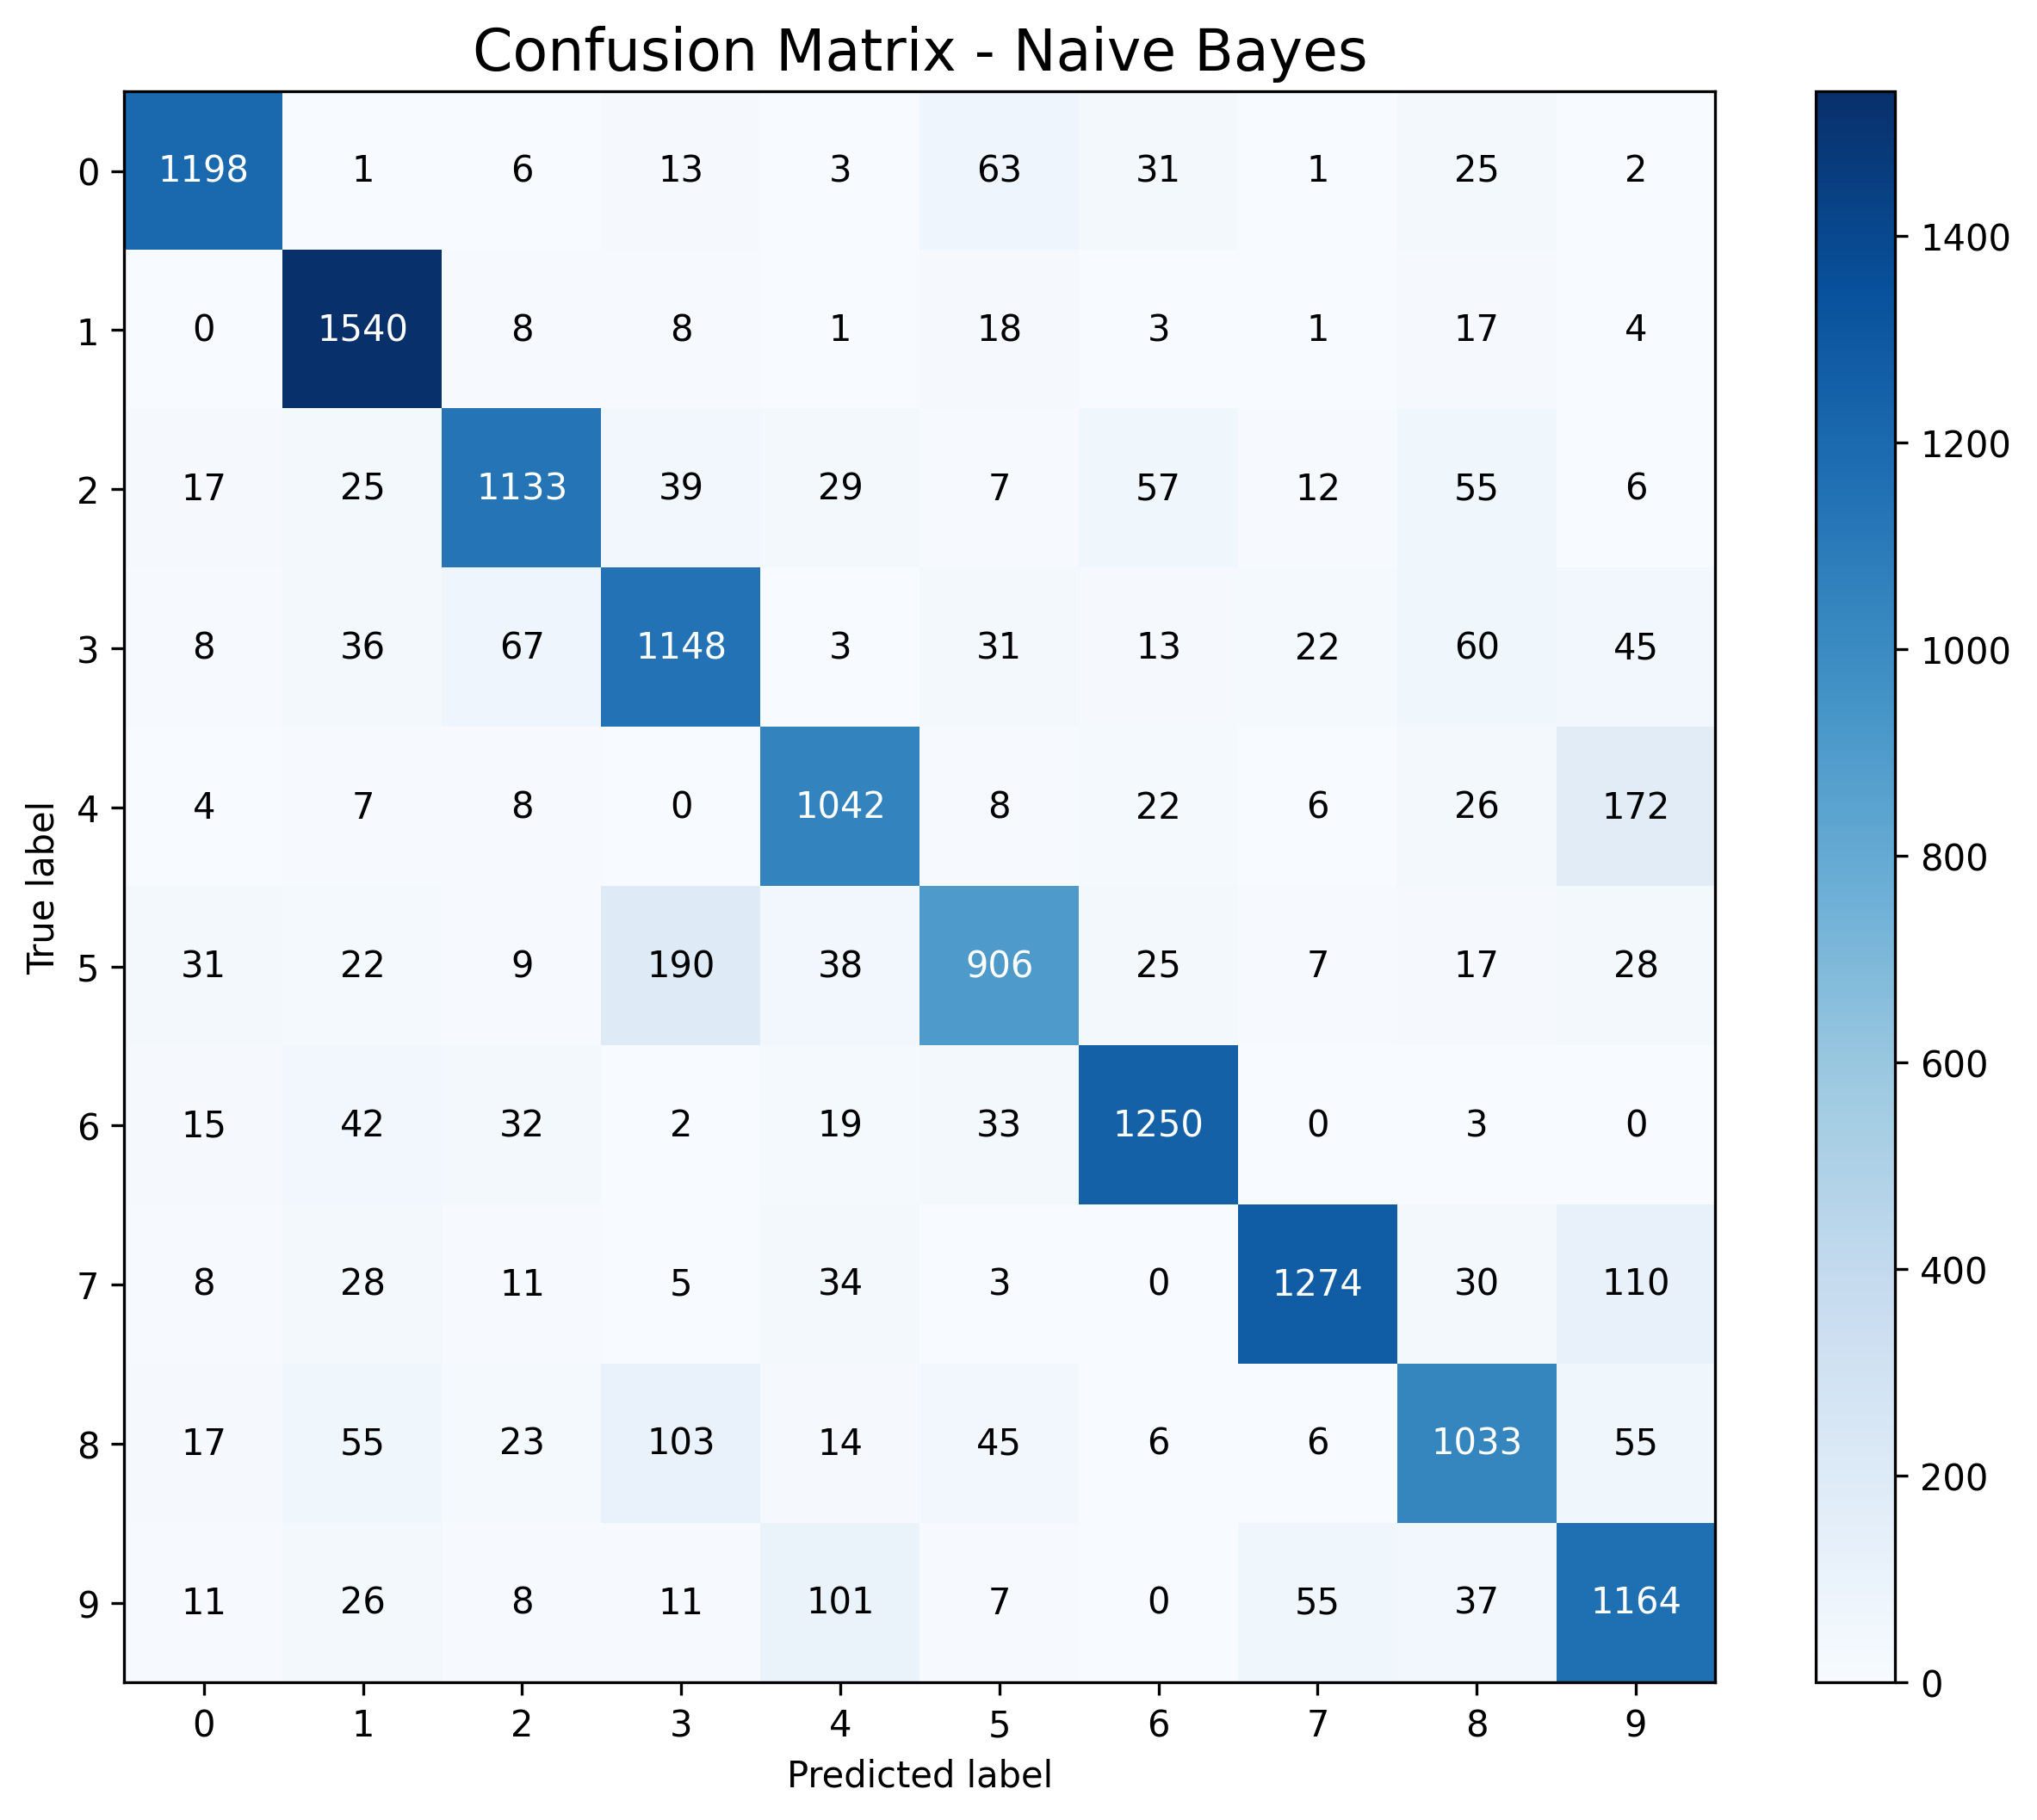
\includegraphics[width=0.8\textwidth]{../figures/3/confusion_matrix_naive_bayes.png}
    \caption{Matriz de confusão do modelo Naive Bayes}
    \label{fig:confusion_matrix}
\end{figure}

\textbf{Análise dos erros mais comuns:}

\begin{table}[H]
    \centering
    \begin{tabular}{|c|c|}
        \hline
        \textbf{Classe} & \textbf{Taxa de Erro (\%)} \\
        \hline
        0               & 10.8                       \\
        1               & 3.8                        \\
        2               & 17.9                       \\
        3               & 19.9                       \\
        4               & 19.5                       \\
        5               & 28.8                       \\
        6               & 10.5                       \\
        7               & 15.2                       \\
        8               & 23.9                       \\
        9               & 18.0                       \\
        \hline
    \end{tabular}
    \caption{Taxa de erro por classe no modelo Naive Bayes}
    \label{tab:error_rates}
\end{table}

A classe mais confundida foi a \textbf{5} (28.8\% de erro). Nota-se pela matriz de confusão que parte considerável dos erros para esta classe ocorreram pois o modelo previu \textbf{3, 0 e 8}. Provavelmente isso acontece pela semelhança visual dos dígitos \textbf{5, 3 e 8} e pelo desbalanceamento da classe \textbf{1} nos dados de treino, que foi a mais frequente (6.277 amostras).

\textbf{Contagem das classes nos dados de treino:}

\begin{table}[H]
    \centering
    \begin{tabular}{|c|c|c|c|c|c|c|c|c|c|c|}
        \hline
        \textbf{Classe}   & 0    & 1    & 2    & 3    & 4    & 5    & 6    & 7    & 8    & 9    \\
        \hline
        \textbf{Contagem} & 5560 & 6277 & 5610 & 5708 & 5529 & 5040 & 5480 & 5790 & 5468 & 5538 \\
        \hline
    \end{tabular}
    \caption{Distribuição das classes no conjunto de treinamento}
    \label{tab:class_distribution}
\end{table}
\newpage

\section*{Exercício 4}
\addcontentsline{toc}{section}{Exercício 4}

\subsection*{Exercício 4a}
\addcontentsline{toc}{subsection}{Exercício 4a}
\section*{Parte (a)}

\subsection*{(a)}
A partir da representação \textit{TF-IDF} dos textos, visualize a similaridade par a par dessa sequência específica (\textit{head\_view}) para interpretar o resultado.

\vspace{0.5em}
\noindent O código implementado para a visualização de atenção dos vetores TF-IDF:

\begin{lstlisting}[language=Python]
# Criação da matriz de atenção usando vetores TF-IDF
import numpy as np
from sklearn.feature_extraction.text import TfidfVectorizer

# Preprocessamento dos dados
scaler = StandardScaler()
X = scaler.fit_transform(np.concatenate([X_train, X_val, X_test]))
X_train_scaled = X[:len(X_train)]
X_val_scaled = X[len(X_train):len(X_train)+len(X_val)]
X_test_scaled = X[len(X_train)+len(X_val):]

# Otimização de hiperparâmetros usando RandomizedSearchCV
param_dist = {
    'max_features': [300, 500, 750, 1000, 1500, 2000],
    'ngram_range': [(1, 1), (1, 2), (1, 3), (2, 2), (2, 3)],
    'min_df': [2, 3, 4, 5],
    'max_df': [0.5, 0.6, 0.7, 0.8, 0.9]
}

best_params = {'max_features': 1000, 'ngram_range': (1, 2), 
               'min_df': 2, 'max_df': 0.9}

# Criação do vetorizador TF-IDF com os melhores parâmetros
vectorizer = TfidfVectorizer(max_features=best_params['max_features'],
                           ngram_range=best_params['ngram_range'],
                           min_df=best_params['min_df'],
                           max_df=best_params['max_df'])

# Aplicação da vetorização TF-IDF
X_train_tfidf = vectorizer.fit_transform(texts_train)
X_test_tfidf = vectorizer.transform(texts_test)

# Seleção dos primeiros 32 exemplos para visualização
b = X_test_tfidf[:32].toarray()
tokens = [f"News {i+1}" for i in range(32)]

# Cálculo da matriz de atenção baseada na similaridade TF-IDF
att = b @ b.T
att = att.reshape(1, 1, 32, 32)
att = torch.tensor(att)

# Visualização usando head_view
head_view((att,), tokens)
\end{lstlisting}

\vspace{0.5em}
\noindent A visualização da matriz de atenção TF-IDF revela os seguintes insights:

\begin{enumerate}
    \item \textbf{Estrutura de blocos}: A matriz apresenta uma estrutura de blocos organizada por classes, indicando que artigos da mesma categoria têm maior similaridade entre si.

    \item \textbf{Interpretação da similaridade}: A intensidade das cores representa a força da relação semântica entre os pares de artigos, onde cores mais intensas indicam maior sobreposição de termos importante segundo a métrica TF-IDF.

    \item \textbf{Padrões observados}: Artigos de categorias distintas apresentam baixa similaridade (regiões escuras), enquanto artigos da mesma categoria mostram maior similaridade (regiões mais claras).
\end{enumerate}
\newpage

\subsection*{Exercício 4b}
\addcontentsline{toc}{subsection}{Exercício 4b}

\section*{Parte (b)}

\subsection*{(b-i)}

Pela definição de projeção ortogonal, temos que
\[
    P_u(v) = \alpha u.
\]

\[
    v - P_u(v) \perp u,
\]
ou seja,
\[
    \langle v - \alpha u, u \rangle = 0.
\]

Expandindo o produto interno,
\[
    \langle v, u \rangle - \alpha \langle u, u \rangle = 0.
\]

Como $\langle u, u \rangle = \|u\|^2$, segue que
\[
    \alpha = \frac{\langle v, u \rangle}{\|u\|^2}.
\]

Portanto,
\[
    P_u(v) = \frac{\langle u, v \rangle}{\|u\|^2}\, u.
\]

\subsection*{(b-ii)}
Considere a definição
\[
    \cos(u,v) := \frac{\langle u, v \rangle}{\|u\|\,\|v\|}.
\]

Pelo item (b-i), a projeção de $v$ sobre $u$ é
\[
    P_u(v) = \frac{\langle u, v\rangle}{\|u\|^2}\, u.
\]

Tomando norma em ambos os lados:
\[
    \|P_u(v)\|
    = \left\|\frac{\langle u, v\rangle}{\|u\|^2} u \right\|
    = \frac{|\langle u, v\rangle|}{\|u\|^2}\,\|u\|
    = \frac{|\langle u, v\rangle|}{\|u\|}.
\]

Dividindo por $\|v\|$, obtemos:
\[
    \frac{\|P_u(v)\|}{\|v\|}
    =
    \frac{|\langle u, v\rangle|}{\|u\|\,\|v\|}.
\]

Logo,
\[
    \cos(u,v)
    =
    \frac{\langle u, v\rangle}{\|u\|\,\|v\|}
    =
    \frac{\|P_u(v)\|}{\|v\|}
    \quad (\text{com sinal dado por } \langle u,v\rangle).
\]

Geometricamente,
\[
    \cos(u,v)
    =
    \frac{\text{cateto adjacente}}{\text{hipotenusa}},
\]
onde $\|P_u(v)\|$ é o cateto adjacente e $\|v\|$ é a hipotenusa.

\subsection*{(b-iii)}


Como os vetores têm norma $1$, vale
\[
    \cos(u,v)=\langle u,v\rangle.
\]

Calculando a norma ao quadrado da diferença:
\[
    \|u-v\|^2
    =
    \langle u-v,\,u-v\rangle.
\]

Expandindo,
\[
    \|u-v\|^2
    =
    \|u\|^2+\|v\|^2-2\langle u,v\rangle.
\]

Como $\|u\|=\|v\|=1$, obtemos
\[
    \|u-v\|^2
    =
    1+1-2\langle u,v\rangle
    =
    2-2\cos(u,v).
\]

Portanto,
\[
    \|u-v\|^2 = 2-2\cos(u,v).
\]

Agora,
\[
    \cos(u_1,v_1)\geq \cos(u_2,v_2)
\]

\[
    \iff
    2-2\cos(u_1,v_1)\leq 2-2\cos(u_2,v_2)
\]

\[
    \iff
    \|u_1-v_1\|^2 \leq \|u_2-v_2\|^2
\]

\[
    \iff
    \|u_1-v_1\| \leq \|u_2-v_2\|.
\]

Logo,
\[
    \cos(u_1,v_1) \geq \cos(u_2,v_2)
    \iff
    \|u_1 - v_1\| \leq \|u_2 - v_2\|.
\]


Para vetores de norma $1$,
\[
    \|u-v\|^2 = 2-2\cos(u,v),
\]
ou seja, o cosseno é uma transformação monótona da distância euclidiana.
Assim, quanto maior $\cos(u,v)$, menor a distância entre os vetores.
Portanto, o cosseno pode ser usado como medida de similaridade para vetores normalizados.

\subsection*{(b-iv)}

\vspace{0.5em}
\noindent A métrica da norma da diferença tem seus valores proporcionais à magnitude dos vetores avaliados. Enquanto isso, a métrica do cosseno pressupõe vetores unitários e é agnóstica à magnitude.

\noindent Assim, em um caso em que apenas a direção importa, o cosseno é preferível. Em casos em que a magnitude também é relevante, a métrica da norma é preferível ao cosseno.

\newpage

\subsection*{Exercício 4c}
\addcontentsline{toc}{subsection}{Exercício 4c}

\section*{Parte (c)}

\subsection*{(c)}
Note que a rede não está aprendendo. Explique qual é o problema e exponha evidências de que ele realmente está acontecendo.

\vspace{0.5em}
\noindent A inicialização incorreta da matriz de pesos é a causa do não aprendizado da rede. Como não normalizamos os pesos, sua variância era grande o suficiente para gerar valores com alta magnitude que, ao passar pelo softmax, resulta em valores próximos a 1 com gradientes próximos a 0.

\vspace{0.5em}
\noindent O problema pode ser observado através das evidências experimentais:

\begin{enumerate}
    \item \textbf{Perda constante}: O gráfico da função perda mostra que ela permanece praticamente constante ao longo das épocas, indicando ausência de aprendizado.

    \item \textbf{Gradientes próximos a zero}: Os histogramas dos gradientes das matrizes $A_K$ e $A_Q$ mostram que a maioria dos gradientes está concentrada em torno de zero, evidenciando o problema do gradiente que desaparece.

    \item \textbf{Saída do softmax saturada}: O histograma da saída do softmax mostra valores próximos a 1, indicando saturação da função.
\end{enumerate}

\begin{figure}[h]
    \centering
    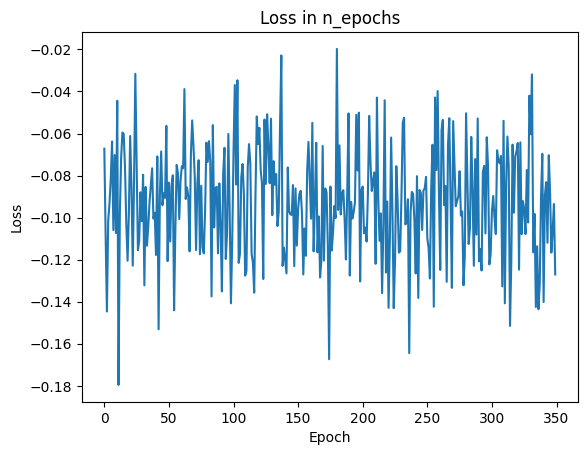
\includegraphics[width=0.7\textwidth]{../figures/4/loss_no_init_fix.png}
    \caption{Função perda sem inicialização adequada - sem aprendizado}
    \label{fig:loss_no_init}
\end{figure}

\begin{figure}[h]
    \centering
    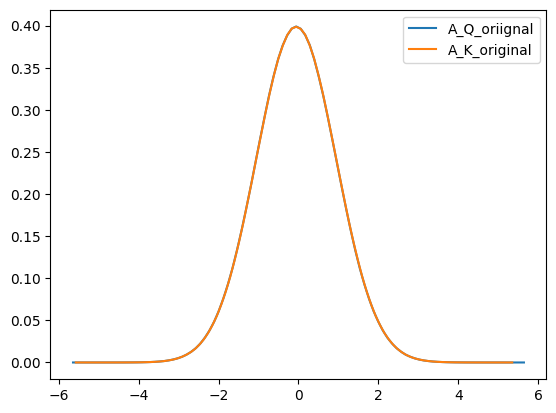
\includegraphics[width=0.7\textwidth]{../figures/4/weight_distributions_no_init_fix.png}
    \caption{Distribuições dos pesos iniciais A\_K e A\_Q}
    \label{fig:weights_no_init}
\end{figure}

\begin{figure}[h]
    \centering
    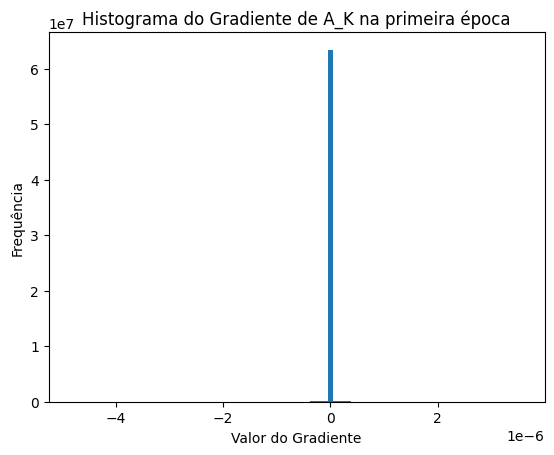
\includegraphics[width=0.45\textwidth]{../figures/4/gradient_histogram_A_K_no_init_fix.png}
    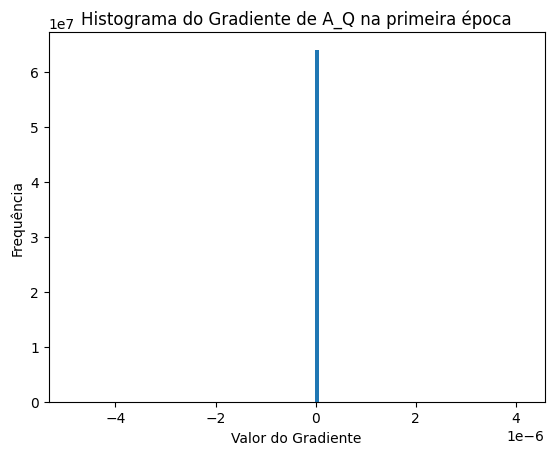
\includegraphics[width=0.45\textwidth]{../figures/4/gradient_histogram_A_Q_no_init_fix.png}
    \caption{Histogramas dos gradientes de A\_K e A\_Q na primeira época (sem inicialização adequada)}
    \label{fig:gradients_no_init}
\end{figure}

\begin{figure}[h]
    \centering
    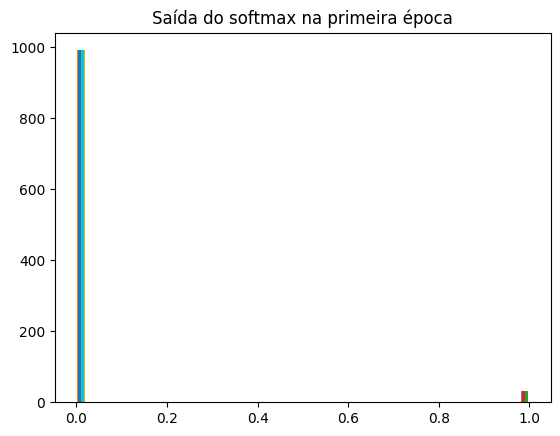
\includegraphics[width=0.7\textwidth]{../figures/4/softmax_output_no_init_fix.png}
    \caption{Saída do softmax na primeira época (sem inicialização adequada)}
    \label{fig:softmax_no_init}
\end{figure}

\vspace{0.5em}
\noindent O c\'{o}digo que demonstra esse problema:

\begin{verbatim}
# Inicialização sem normalização adequada
A_K = torch.randn((D,D)).cuda()  # SEM *init_scale(D)
A_Q = torch.randn((D,D)).cuda()  # SEM *init_scale(D)

# Loop de treinamento
for epoch in range(n_epochs):
    # ... treinamento ...
    att = softmax((K.T@Q)/(D**(1/2)))
    loss = -cos(att,truth).mean()
    loss.backward()
\end{verbatim}

\newpage

\subsection*{Exercício 4d}
\addcontentsline{toc}{subsection}{Exercício 4d}

\section*{Parte (d)}

\subsection*{(d)}
Corrija o problema identificado no item anterior e demonstre que a rede agora consegue aprender.

\vspace{0.5em}
\noindent De fato, adicionar um termo na inicialização dos parâmetros permitiu o aprendizado e subsequente redução da função perda. Isso ocorre pois o valor pelo qual multiplicamos os pesos iniciais é $(2/D)^{1/2}$, sendo $D$ o tamanho da camada. Isso reduz a variância dos parâmetros e evita que valores muito grandes sejam passados ao softmax e tenham seu gradiente próximo a zero.

\vspace{0.5em}
\noindent A correção implementada:

\begin{verbatim}
def init_scale(fan_in):
    return (2/fan_in)**0.5

# Inicialização com normalização adequada
A_K = torch.randn((D,D)).cuda() * init_scale(D)  # COM *init_scale(D)
A_Q = torch.randn((D,D)).cuda() * init_scale(D)  # COM *init_scale(D)
\end{verbatim}

\vspace{0.5em}
\noindent As evidências do aprendizado bem-sucedido incluem:

\begin{enumerate}
    \item \textbf{Redução da perda}: O gráfico da função perda agora mostra uma tendência decrescente clara ao longo das épocas.

    \item \textbf{Gradientes não-zero}: Os histogramas dos gradientes mostram distribuições mais amplas, indicando gradientes efetivos para o aprendizado.

    \item \textbf{Distribuição melhorada do softmax}: A saída do softmax apresenta uma distribuição mais balanceada, não saturada.
\end{enumerate}

\begin{figure}[h]
    \centering
    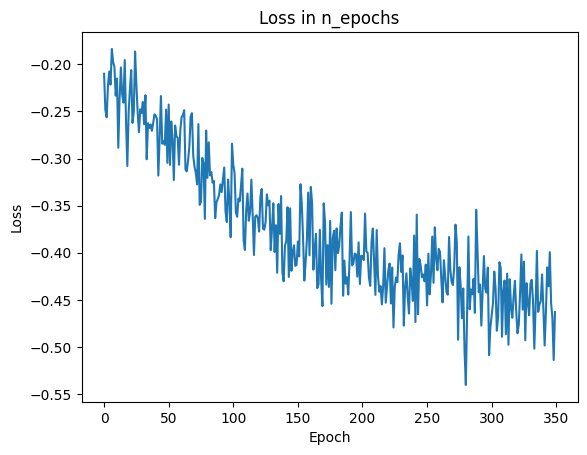
\includegraphics[width=0.7\textwidth]{../figures/4/loss_with_init_fix.png}
    \caption{Função perda com inicialização adequada - aprendizado bem-sucedido}
    \label{fig:loss_with_init}
\end{figure}

\begin{figure}[h]
    \centering
    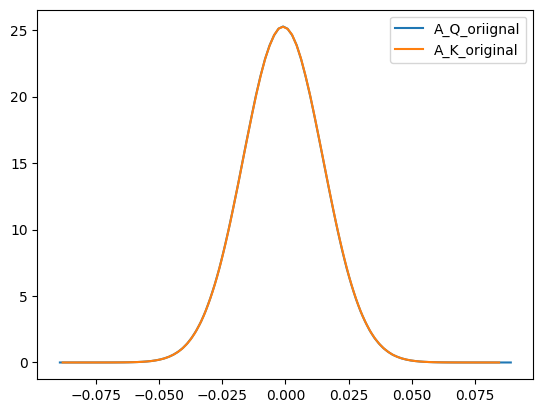
\includegraphics[width=0.7\textwidth]{../figures/4/weight_distributions_with_init_fix.png}
    \caption{Distribuições dos pesos iniciais A\_K e A\_Q com inicialização adequada}
    \label{fig:weights_with_init}
\end{figure}

\begin{figure}[h]
    \centering
    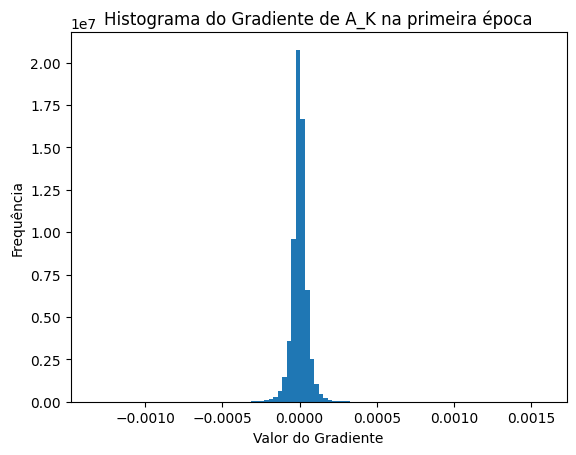
\includegraphics[width=0.45\textwidth]{../figures/4/gradient_histogram_A_K_with_init_fix.png}
    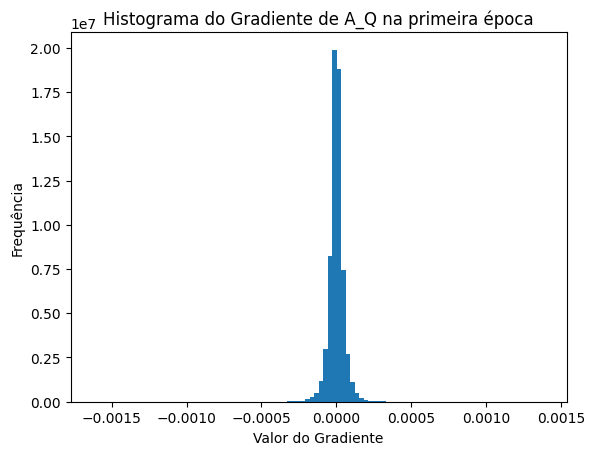
\includegraphics[width=0.45\textwidth]{../figures/4/gradient_histogram_A_Q_with_init_fix.png}
    \caption{Histogramas dos gradientes de A\_K e A\_Q na primeira época (com inicialização adequada)}
    \label{fig:gradients_with_init}
\end{figure}

\begin{figure}[h]
    \centering
    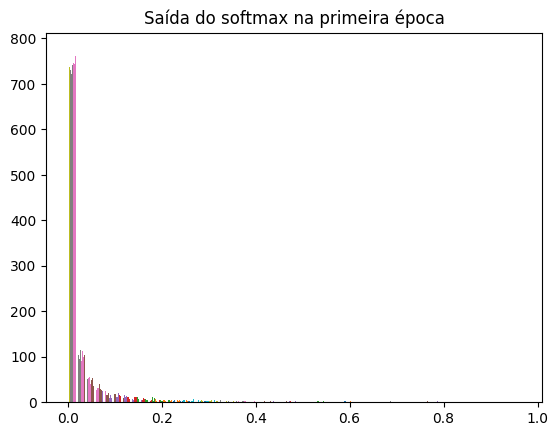
\includegraphics[width=0.7\textwidth]{../figures/4/softmax_output_with_init_fix.png}
    \caption{Saída do softmax na primeira época (com inicialização adequada)}
    \label{fig:softmax_with_init}
\end{figure}


\newpage

\subsection*{Exercício 4e}
\addcontentsline{toc}{subsection}{Exercício 4e}
\section*{Parte (e)}

\subsection*{(e-i)}
A camada de auto-atenção (self-attention) pode ser representada matematicamente como
\begin{equation*}
    \text{Sa}[X] = V[X] \cdot \text{Softmax} \left( \frac{K[X]^T Q[X]}{\sqrt{D}} \right)
\end{equation*}
Mostre que, se $K[X]$ e $Q[X]$ têm entradas gaussianas com média zero e variância $\sigma^2$, todas independentes entre si, cada entrada de $K[X]^T Q[X]$ tem variância $\sigma^4 D$. Use esse fato para argumentar a favor da divisão por $\sqrt{D}$.

\vspace{0.5em}
\noindent Seja $Z = K[X]^T Q[X] = \sum_{i=1}^D K_i[X]^T Q_i[X]$

\noindent Calculando a Esperança $\mathbb{E}(Z)$:
\begin{align*}
    \mathbb{E}(Z) & = \mathbb{E}(K[X]^T Q[X])                                                         \\
                  & = \mathbb{E}(K[X]^T) \cdot \mathbb{E}(Q[X]) \quad \text{(devido à independência)} \\
                  & = 0 \cdot 0 = 0
\end{align*}

\noindent Calculando a Variância $\mathbb{V}(Z)$:
\begin{align*}
    \mathbb{V}(Z) & = \mathbb{V}(K[X]^T Q[X])                                                 \\
                  & = \mathbb{E}\left([K[X]^T Q[X] - \mathbb{E}(K[X]^T Q[X])]^2\right)        \\
                  & = \mathbb{E}\left((K[X]^T Q[X])^2\right) - (\mathbb{E}(K[X]^T Q[X]))^2    \\
                  & = \mathbb{E}\left((K[X]^T)^2\right) \cdot \mathbb{E}\left((Q[X])^2\right)
\end{align*}

\noindent Como $\mathbb{V}(K[X]^T) = \mathbb{E}\left((K[X]^T)^2\right) - (\mathbb{E}[K[X]^T])^2$:
\begin{equation*}
    \mathbb{V}(K[X]^T) = \mathbb{E}\left((K[X]^T)^2\right)
\end{equation*}

\noindent Logo, $\mathbb{V}(Z) = \mathbb{V}(K[X]^T) \cdot \mathbb{V}(Q[X])$

\noindent A variância de cada termo na soma é $\sigma^2 \cdot \sigma^2 = \sigma^4$. Somando sobre as $D$ dimensões:
\begin{equation*}
    \mathbb{V}(Z)_{ij} = \sum_{i=1}^D \sigma^4 = D\sigma^4
\end{equation*}

\noindent Para normalizarmos e obtermos variância unitária, devemos dividir pela raiz da variância. Como $\sigma$ é comum a ambos os termos da divisão, apenas $\sqrt{D}$ aparece no denominador.

\subsection*{(e-ii)}
É necessário assumir que as entradas são gaussianas para chegar a essa conclusão? Caso contrário, é necessário que sejam identicamente distribuídas?

\vspace{0.5em}
\noindent Não foi necessário assumir distribuição gaussiana das variáveis, apenas independência e mesmos valores de média e variância. Os mesmos resultados seriam obtidos caso as variáveis não seguissem a mesma distribuição, mas mantivessem a independência e os valores de média e variância constantes.
\newpage

\subsection*{Exercício 4f}
\addcontentsline{toc}{subsection}{Exercício 4f}
\begin{lstlisting}[language=Python]
att = (A_K.cpu().detach().numpy()@b.T ).T @ (A_Q.cpu().detach().numpy()@b.T )
att = att.reshape(1,1,32,32)
att = torch.tensor(att)
head_view((att,), tokens)
\end{lstlisting}


\vspace{0.5em}
\begin{figure}[h]
    \centering
    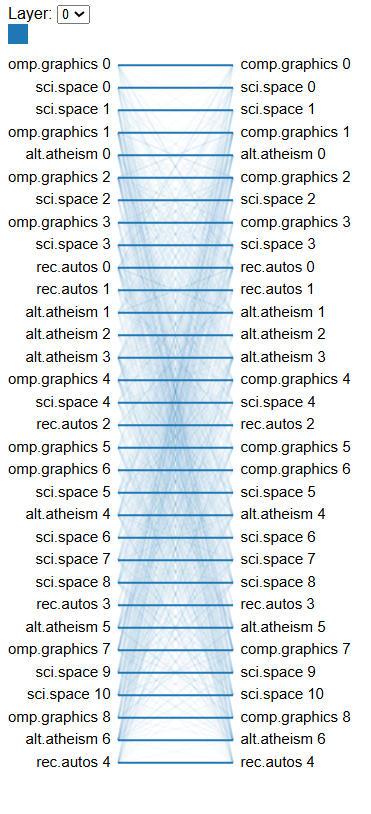
\includegraphics[width=0.45\textwidth]{../figures/4/attention_begin.png}
    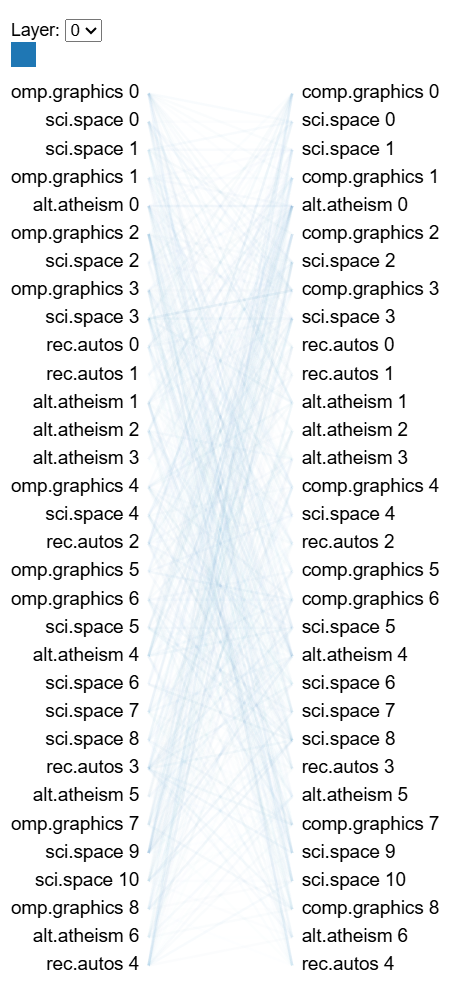
\includegraphics[width=0.45\textwidth]{../figures/4/attention_learned.png}
    \caption{Comparação entre a visualização de atenção inicial (TF-IDF) e após o treinamento (atenção aprendida)}
    \label{fig:attention_comparison}
\end{figure}

\vspace{0.5em}
\noindent O resultado do presente head\_view apresenta relações entre amostras da mesma classe mais fortes que o head\_view do item (a), indicando o impacto do treinamento na definição da similaridade.
\noindent A comparação entre as visualizações mostra que a rede aprendeu a criar representações que aumentam a similaridade entre artigos da mesma categoria, demonstrando que o mecanismo de atenção pode aprender padrões mais sofisticados que a simples sobreposição de termos.
\noindent Isso implica em uma matriz mais esparsa e focada, onde as relações entre amostras da mesma classe são ressaltadas.


\newpage

\subsection*{Exercício 4g}
\addcontentsline{toc}{subsection}{Exercício 4g}
A matriz V e o Multi-head Attention são úteis para problemas em que múltiplas relações são relevantes para a relação entre as amostras. O Multi-head Attention
permite que a rede aprenda diferentes dimensões da similaridade entre as amostras, enquanto a matriz V pode ser usada para aprender as relações entre multiplas amostras.
No caso do presente exercício, apenas as relações par a par foram consideradas. Em problemas em que vários textos são comparados, a matriz V pode ser útil.
Já para problemas onde busca-se representar sintaxe e semântica, o Multi-head Attention é adequado.

\newpage

\section*{Exercício 5}
\addcontentsline{toc}{section}{Exercício 5}

\subsection*{Exercício 5a}
\addcontentsline{toc}{subsection}{Exercício 5a}
\begin{lstlisting}[language=Python]
import numpy as np
import matplotlib.pyplot as plt
import matplotlib.image as mpimg
from sklearn.cluster import KMeans

def function_1(img, parameter):
    temp = np.reshape(img, (img.shape[0] * img.shape[1], 3))
    model = KMeans(n_clusters=parameter, random_state=0, n_init=1).fit(temp)
    output = model.cluster_centers_[model.labels_]
    output = np.reshape(output, (img.shape[0], img.shape[1], 3))
    return output

imagem = mpimg.imread("data/araras.png")
output = function_1(imagem, 3)
# Plotagem das figuras 1, 2 e 3
\end{lstlisting}

\begin{figure}[H]
    \centering
    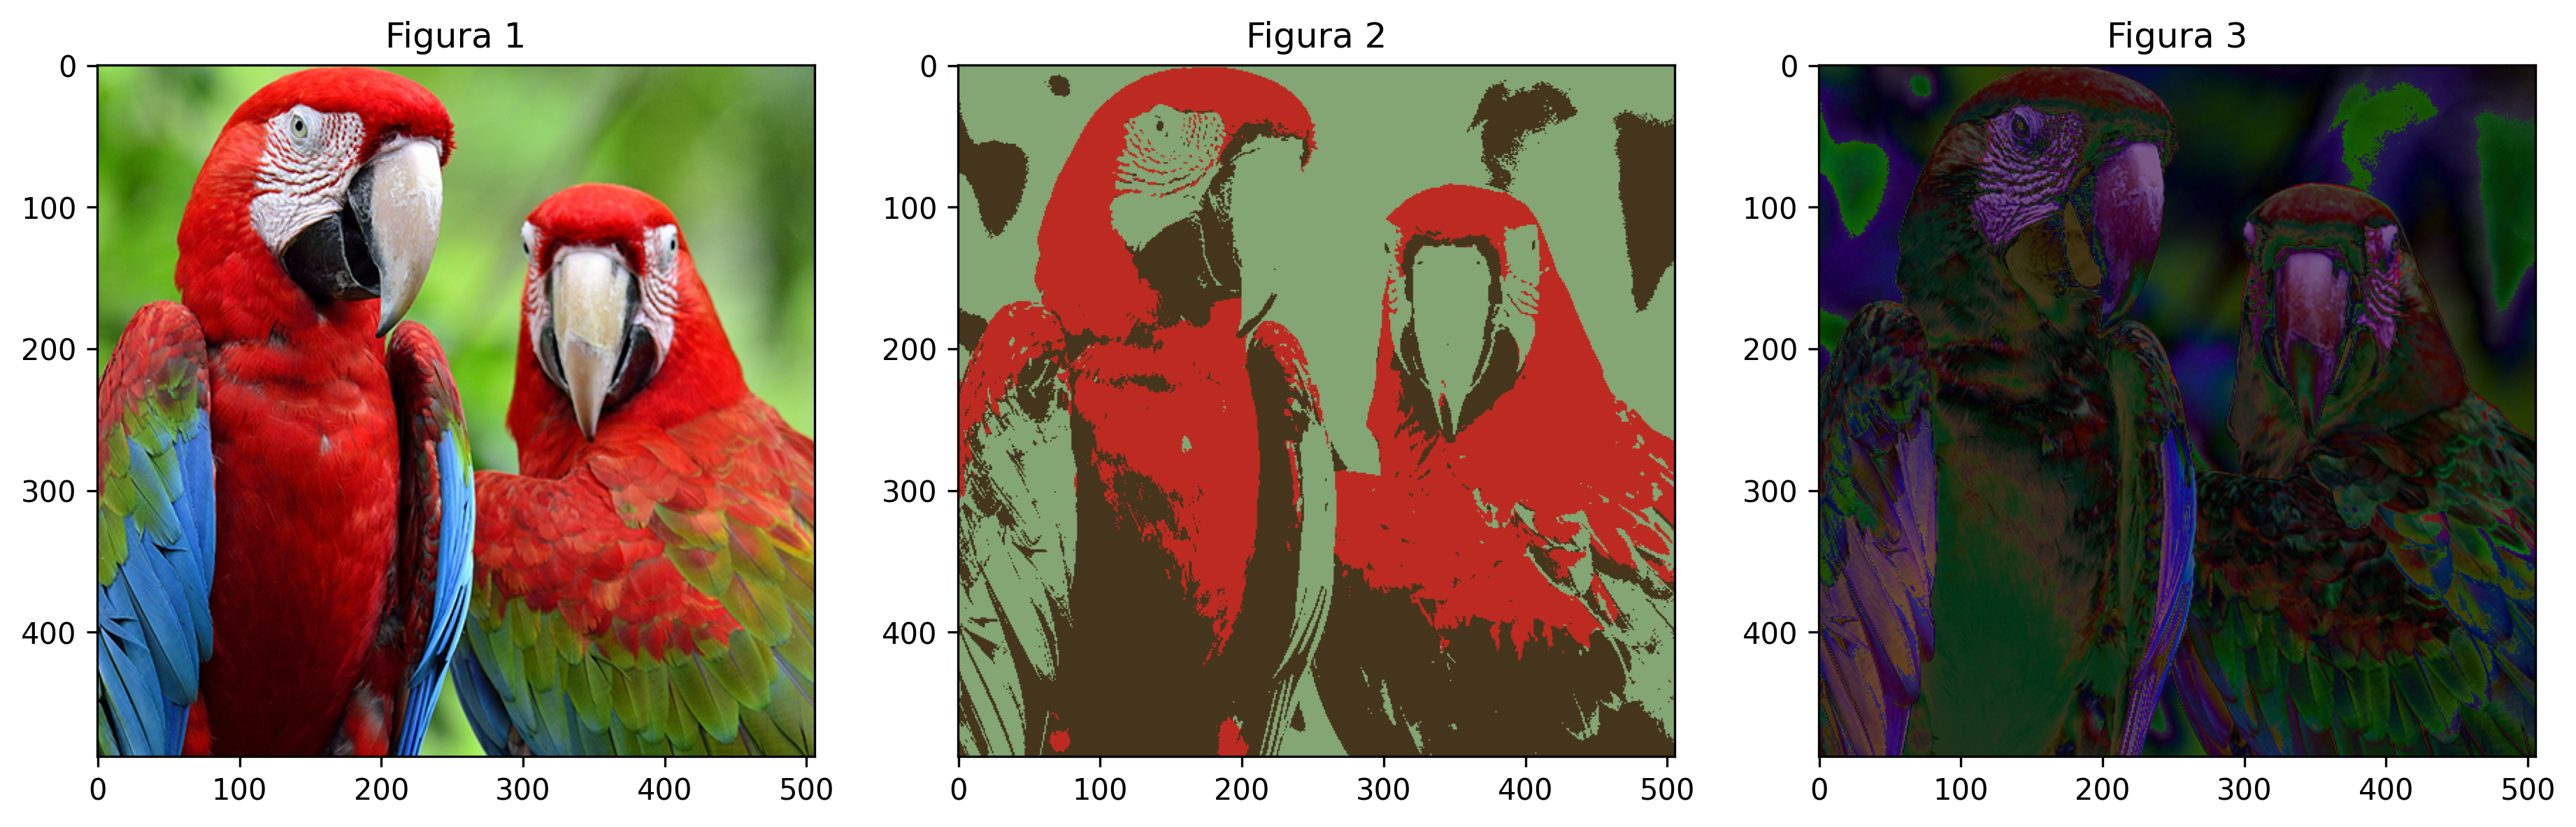
\includegraphics[width=0.9\textwidth]{../figures/5/initial_demo_k3.png}
    \caption{Demonstração inicial do algoritmo K-means com k=3}
    \label{fig:demo_k3}
\end{figure}

\newpage

\begin{lstlisting}[language=Python]
parameters = [3, 10, 30]
for parameter in parameters:
    output = function_1(imagem, parameter)
    # Plotagem das tres figuras para cada valor de parameter
\end{lstlisting}


\begin{figure}[H]
    \centering
    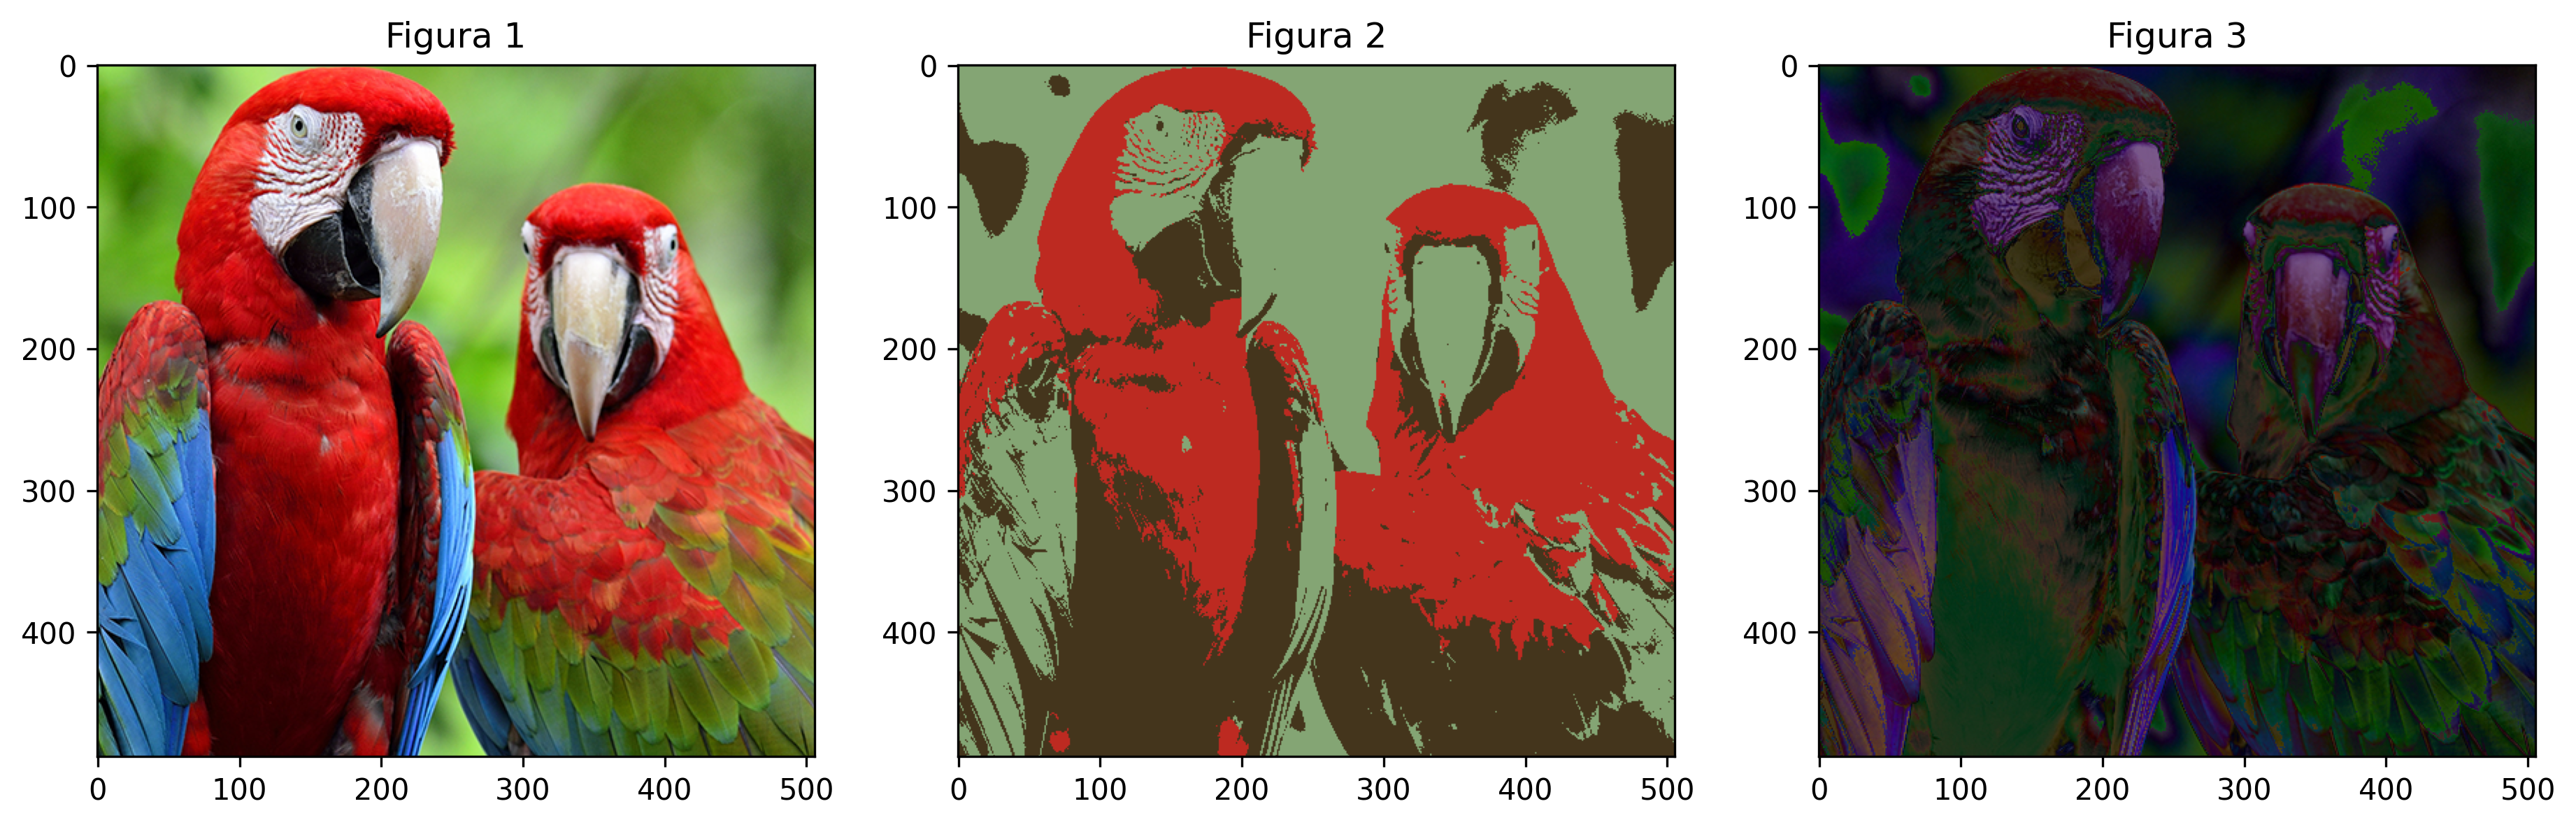
\includegraphics[width=0.9\textwidth]{../figures/5/parameter_3.png}
    \caption{Resultado com parameter = 3}
    \label{fig:param_3}
\end{figure}

\begin{figure}[H]
    \centering
    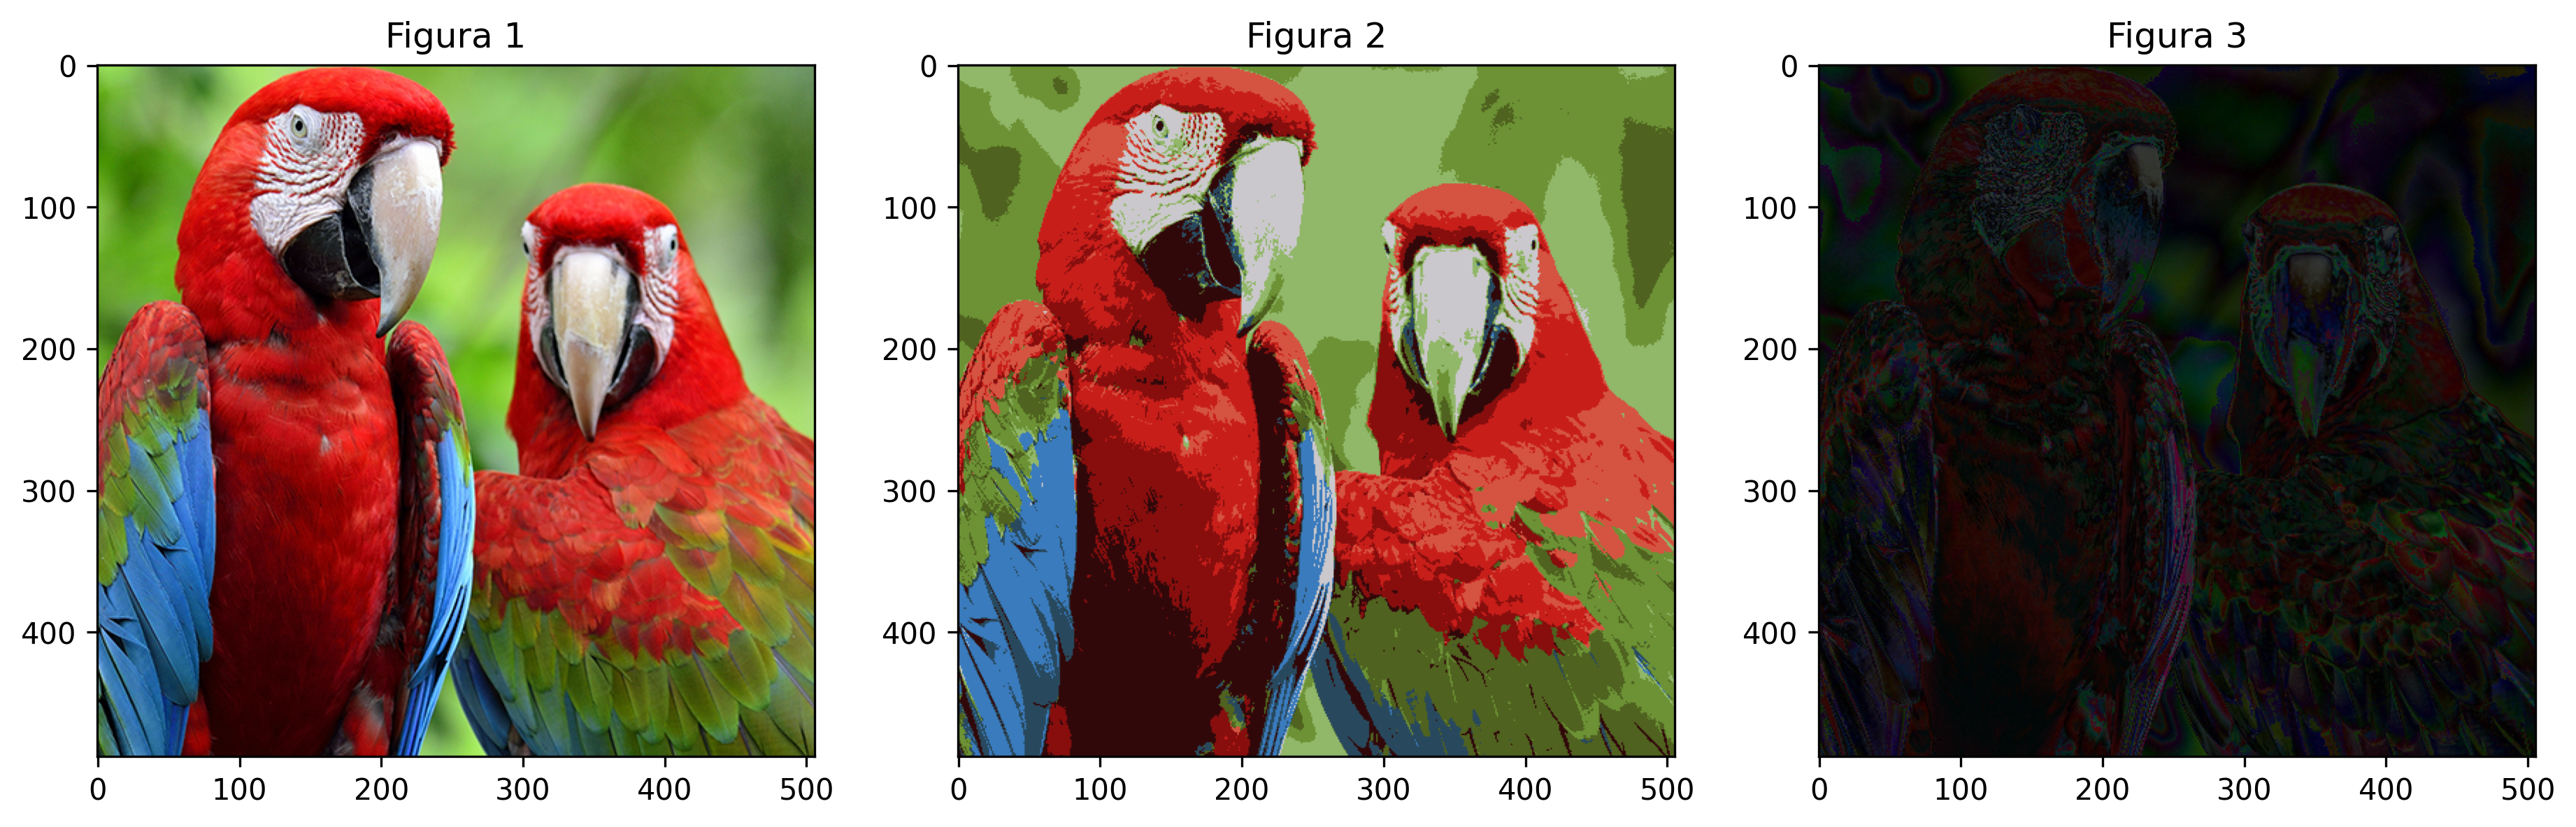
\includegraphics[width=0.9\textwidth]{../figures/5/parameter_10.png}
    \caption{Resultado com parameter = 10}
    \label{fig:param_10}
\end{figure}

\begin{figure}[H]
    \centering
    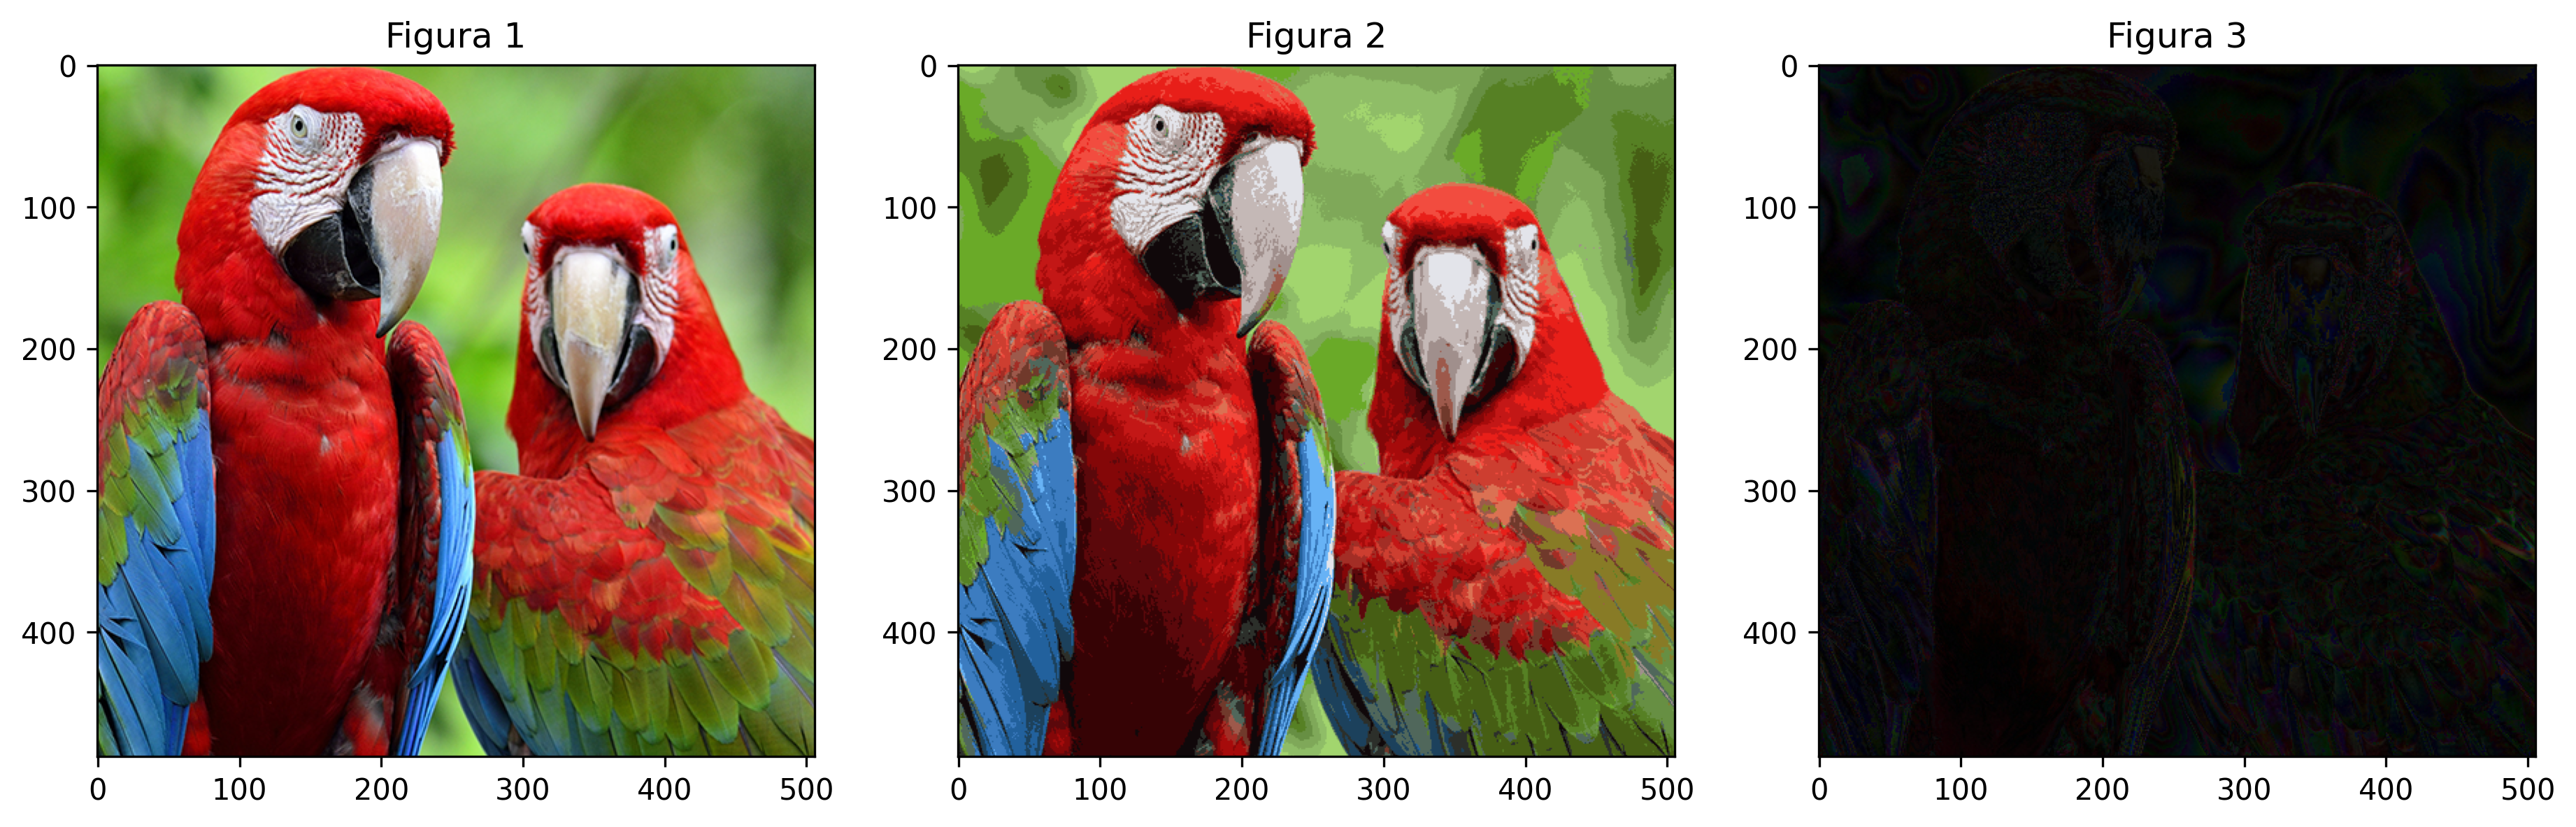
\includegraphics[width=0.9\textwidth]{../figures/5/parameter_30.png}
    \caption{Resultado com parameter = 30}
    \label{fig:param_30}
\end{figure}


A Figura 1 é a imagem original. A Figura 2 é a classificação de cada pixel em um dos três clusteres analisados. Cada cluster representa uma das três cores que melhor agrupavam as amostras em três grupos. A figura 3 é a parte da imagem que não foi incorporada na classificação anterior. Nela, foi retirado de cada pixel o cluster no qual ele foi classificado.

O \texttt{parameter} representa o número de clusteres que serão considerados na decomposição da imagem. Quanto maior o número de clusteres, mais cores serão consideradas na classificação, e a imagem resultante da Figura 2 se aproximará mais da imagem original. Já a Figura 3 se aproximará de uma imagem completamente preta, pois cada vez menos pixels serão classificados como parte do cluster errado.

\newpage

\subsection*{Exercício 5b}
\addcontentsline{toc}{subsection}{Exercício 5b}
\subsection*{Item b}
\addcontentsline{toc}{subsection}{Item b}

Cada classe terá a cor armazenada em uma matriz separada de tamanho 24*parameter. Para representar a classe de cada pixel para reproduzir
a imagem, precisa-se representar apenas o índice da classe. Dessa forma, o número de bits por pixel necessários será Assim, o número de bits por pixel necessários é dado por
\[
    \lceil \log_{2}(\text{parameter}) \rceil
\]

A função teto $\lceil \cdot \rceil$ garante que o número de bits seja inteiro e suficientes para representar as classes.
\newpage

\subsection*{Exercício 5c}
\addcontentsline{toc}{subsection}{Exercício 5c}
\subsection*{Item c}
\addcontentsline{toc}{subsection}{Item c}

\begin{lstlisting}[language=Python]
parameter_interval = np.array(range(2, 50, 5))
image = mpimg.imread("data/araras.png")

# Geracao das imagens comprimidas
for i in parameter_interval:
    tmp = function_1(image, i)
    plt.imsave(f"../results/imagem_{i}.png", tmp)

# Calculo das taxas de compressao
original_size = os.path.getsize("data/araras.png")
sizes = []
for i in parameter_interval:
    file_size = os.path.getsize(f"../results/imagem_{i}.png")
    sizes.append(file_size / original_size)

theoretical_sizes = np.ceil(np.log2(parameter_interval)) / 24

# Plotagem das curvas real vs teorica
\end{lstlisting}

\begin{figure}[H]
    \centering
    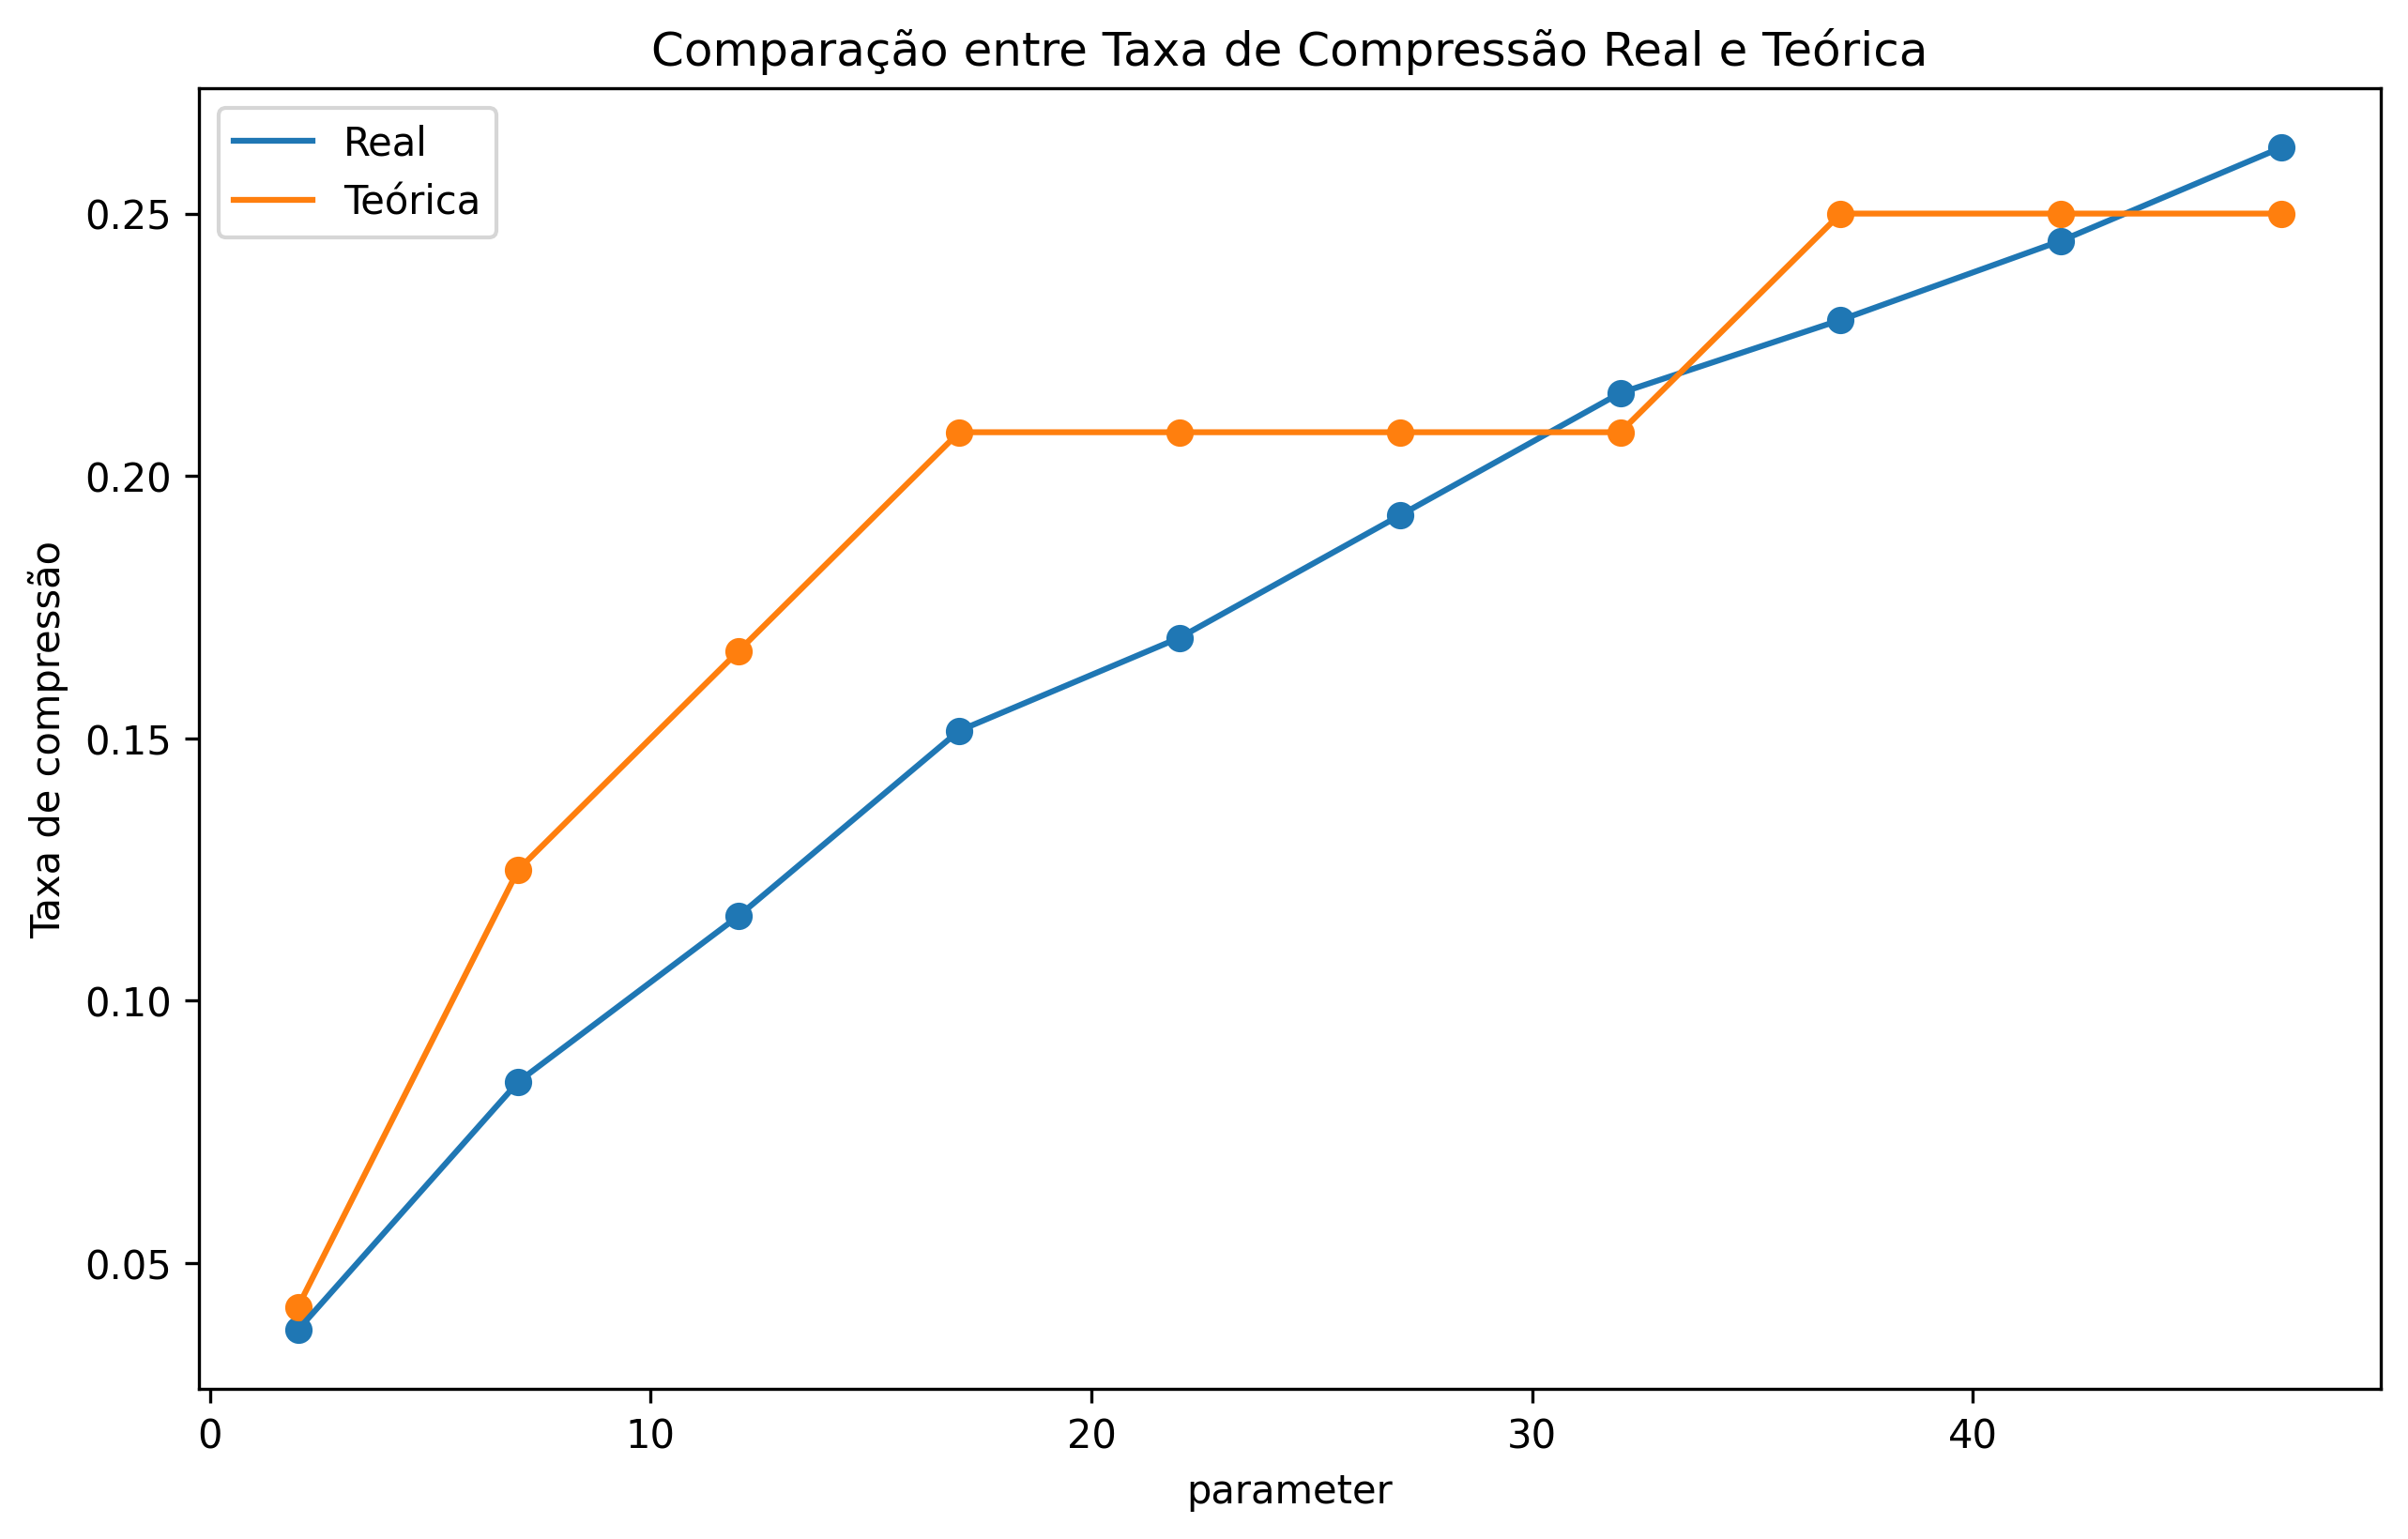
\includegraphics[width=0.8\textwidth]{../figures/5/compression_rates.png}
    \caption{Comparação entre taxa de compressão real e teórica}
    \label{fig:compression_rates}
\end{figure}


A taxa de compressão verificada é calculada considerando o arquivo em toda a sua extensão, o que inclui seus metadados, headers e técnicas de compressão do formato PNG.
Em contrapartida, os valores teóricos consideravam apenas a equivalência bit a bit, não considerando a matriz com o armazenamento das classes. Caso fosse considerada,
ela adicionaria um termo $\frac{\text{parameter}}{\text{num\_pixels}}$ ao valor teórico da taxa de compressão, o que, para o caso desta imagem, seria próximo a 0.

Assim, a taxa de compressão real foi menor do que a taxa teórica para valores baixos de parameter, o que pode ser explicado pelas técnicas de compressão
adotadas pelo formato PNG, que são mais eficientes para imagens com menos variação de cores e a menor quantidade de headers.

À medida que o número de clusters aumenta, a taxa de compressão verificada se aproxima da taxa teórica, até que esta torna-se mais eficiente para valores mais
altos de parameter. Isso pode ser explicado pela presença de maior quantidade de metadados e menor eficiência das técnicas de compressão do formato PNG para
imagens com maior variação de cores.
\newpage

\subsection*{Exercício 5d}
\addcontentsline{toc}{subsection}{Exercício 5d}


\begin{lstlisting}[language=Python]
def function_2(img, parameter):
    temp = np.reshape(img, (img.shape[0] * img.shape[1], 3))
    model = KMeans(n_clusters=parameter, random_state=0, n_init=1).fit(temp)
    return model.inertia_

within_cluster_variation = []
for i in parameter_interval:
    image = mpimg.imread("data/araras.png")
    within_cluster_variation.append(function_2(image, i))
\end{lstlisting}

O valor \texttt{model.inertia\_} representa a soma dos quadrados das distâncias dos pontos até o centro do cluster em que se encontram.

\begin{figure}[H]
    \centering
    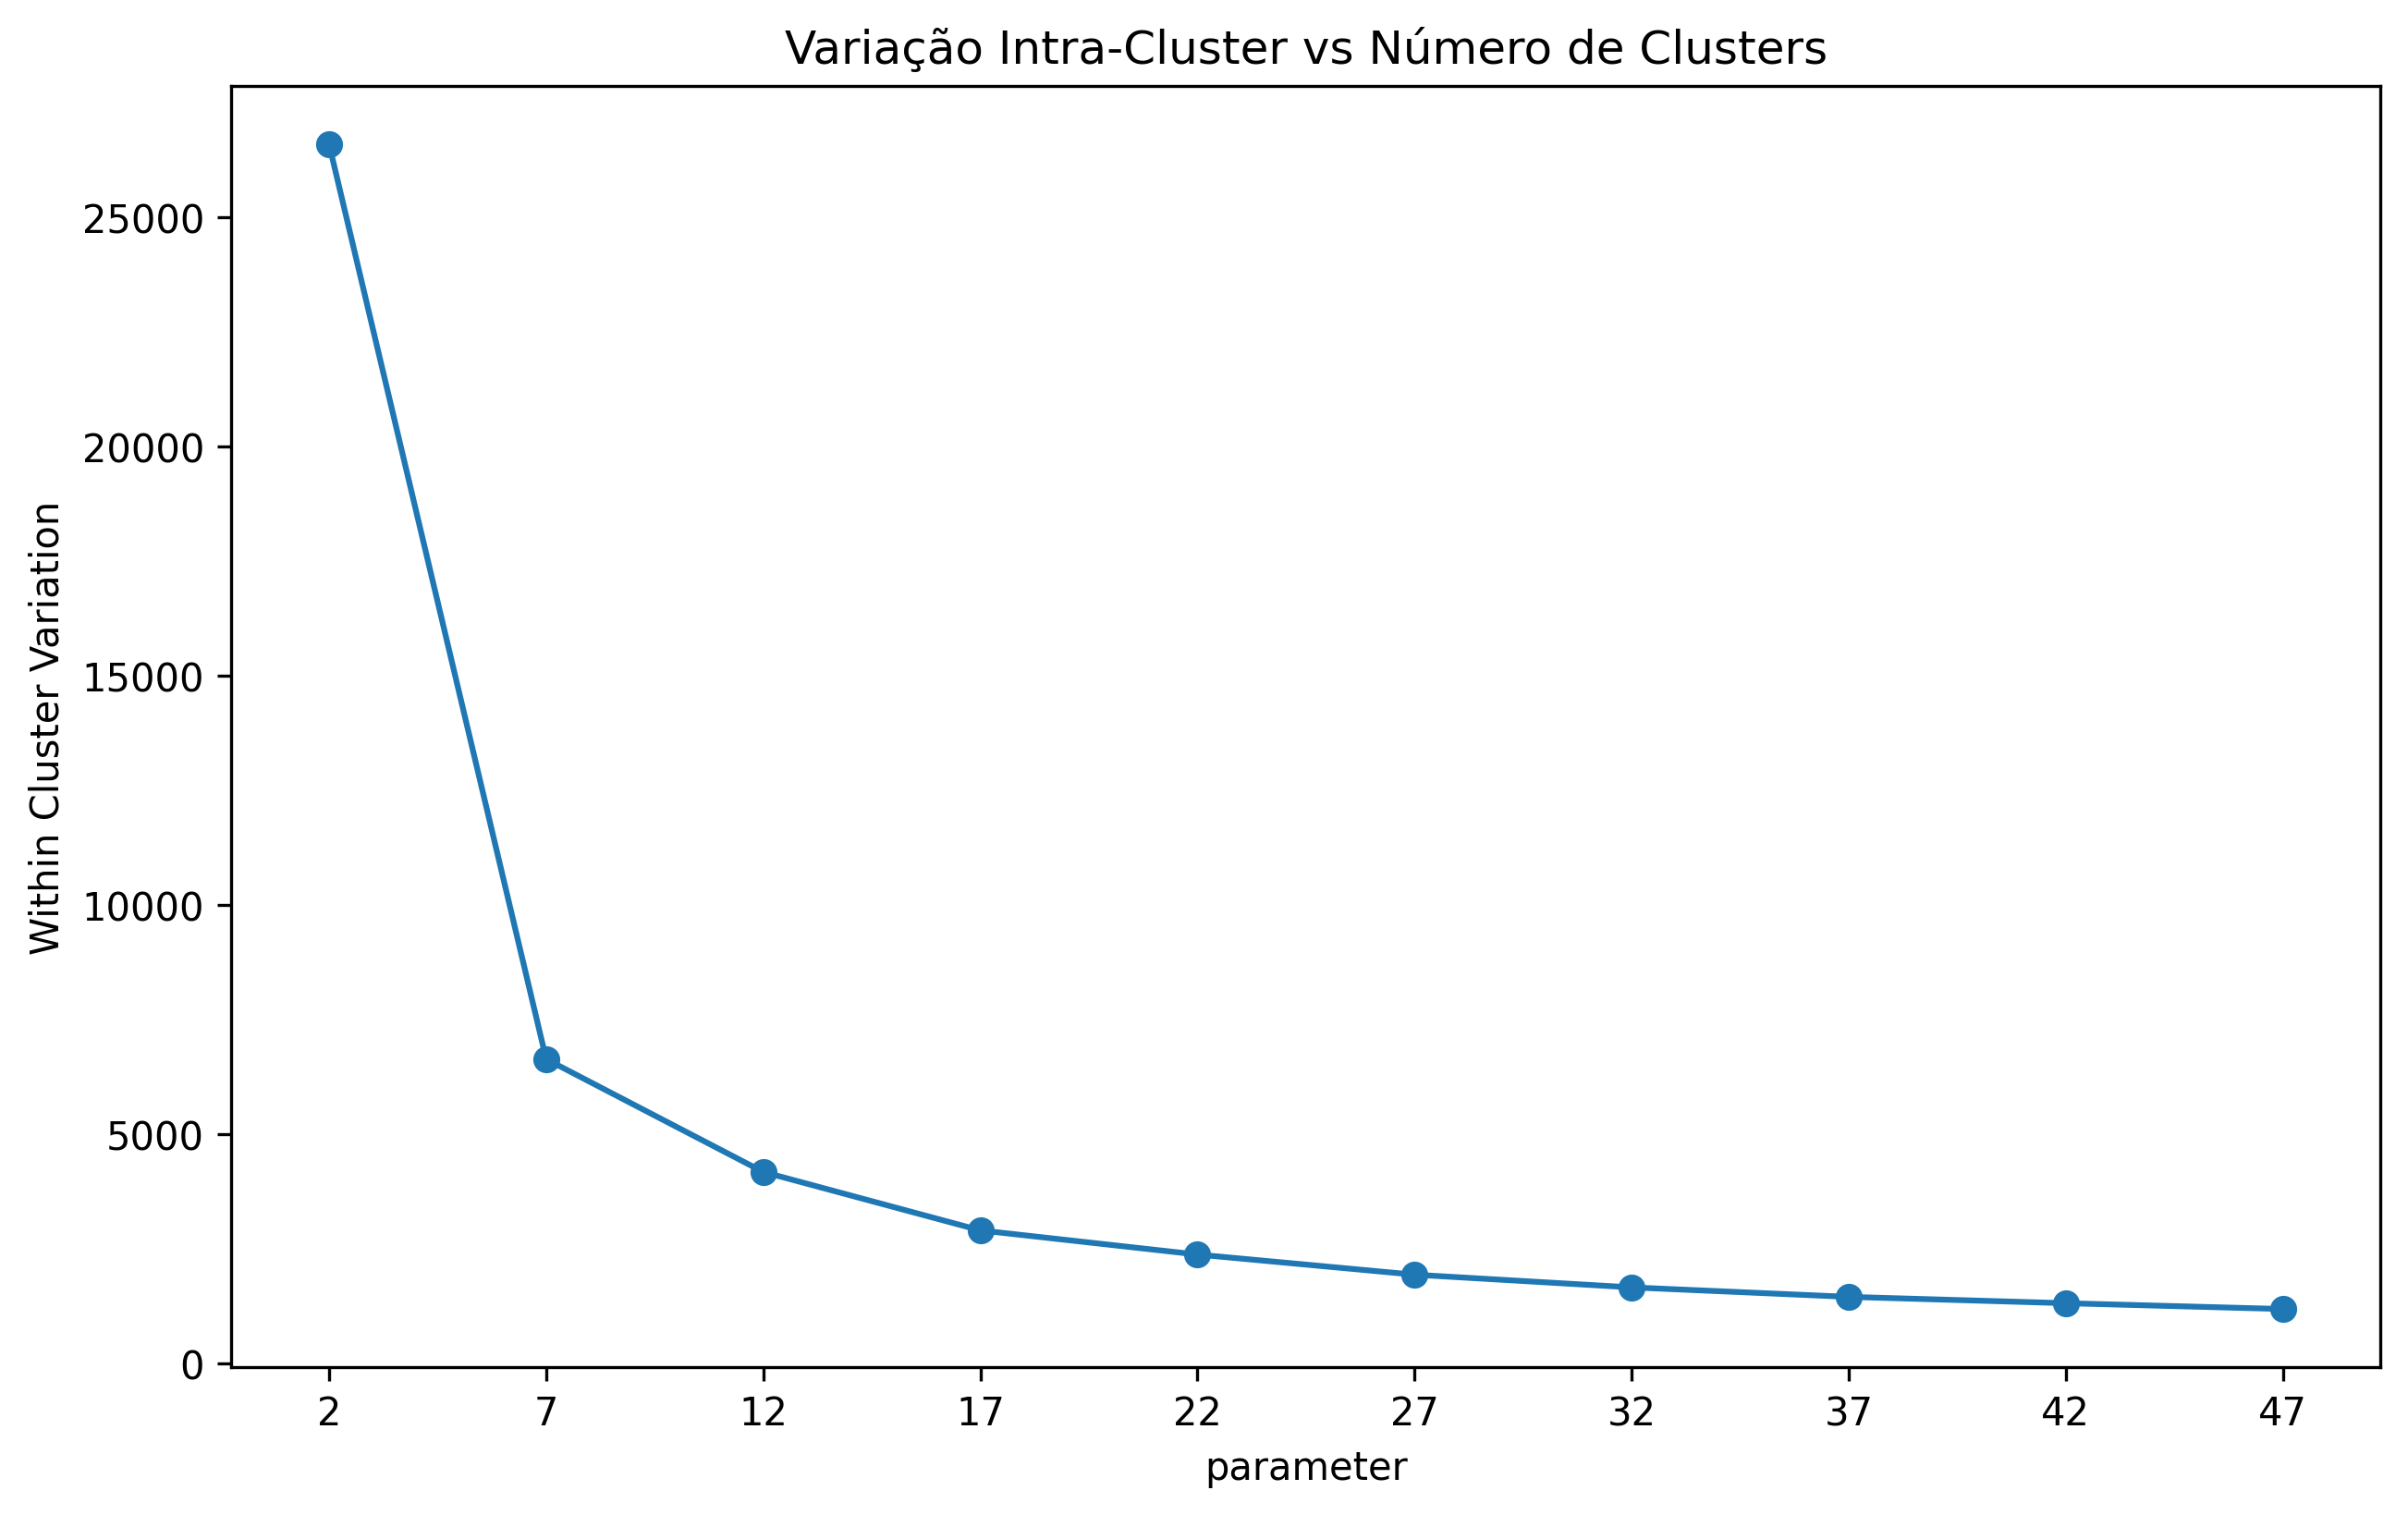
\includegraphics[width=0.8\textwidth]{../figures/5/within_cluster_variation.png}
    \caption{Variação intra-cluster vs número de clusters (método do cotovelo)}
    \label{fig:elbow_method}
\end{figure}

\textbf{Escolha do número de clusters:}

Considerando o gráfico, um valor de k apropriado para o problema seria 12. A partir deste ponto, a distância média entre os pontos de uma classe e o centro do cluster reduz menos com o aumento do número de centróides. Antes dele, essa distância era grande demais.

Em outras palavras, o trade-off entre compressão e reprodutibilidade teria um "joelho" neste ponto. Intuitivamente, usaríamos esse gráfico identificando o ponto onde a curva muda de comportamento (de decréscimo acentuado para decréscimo gradual).

\begin{figure}[H]
    \centering
    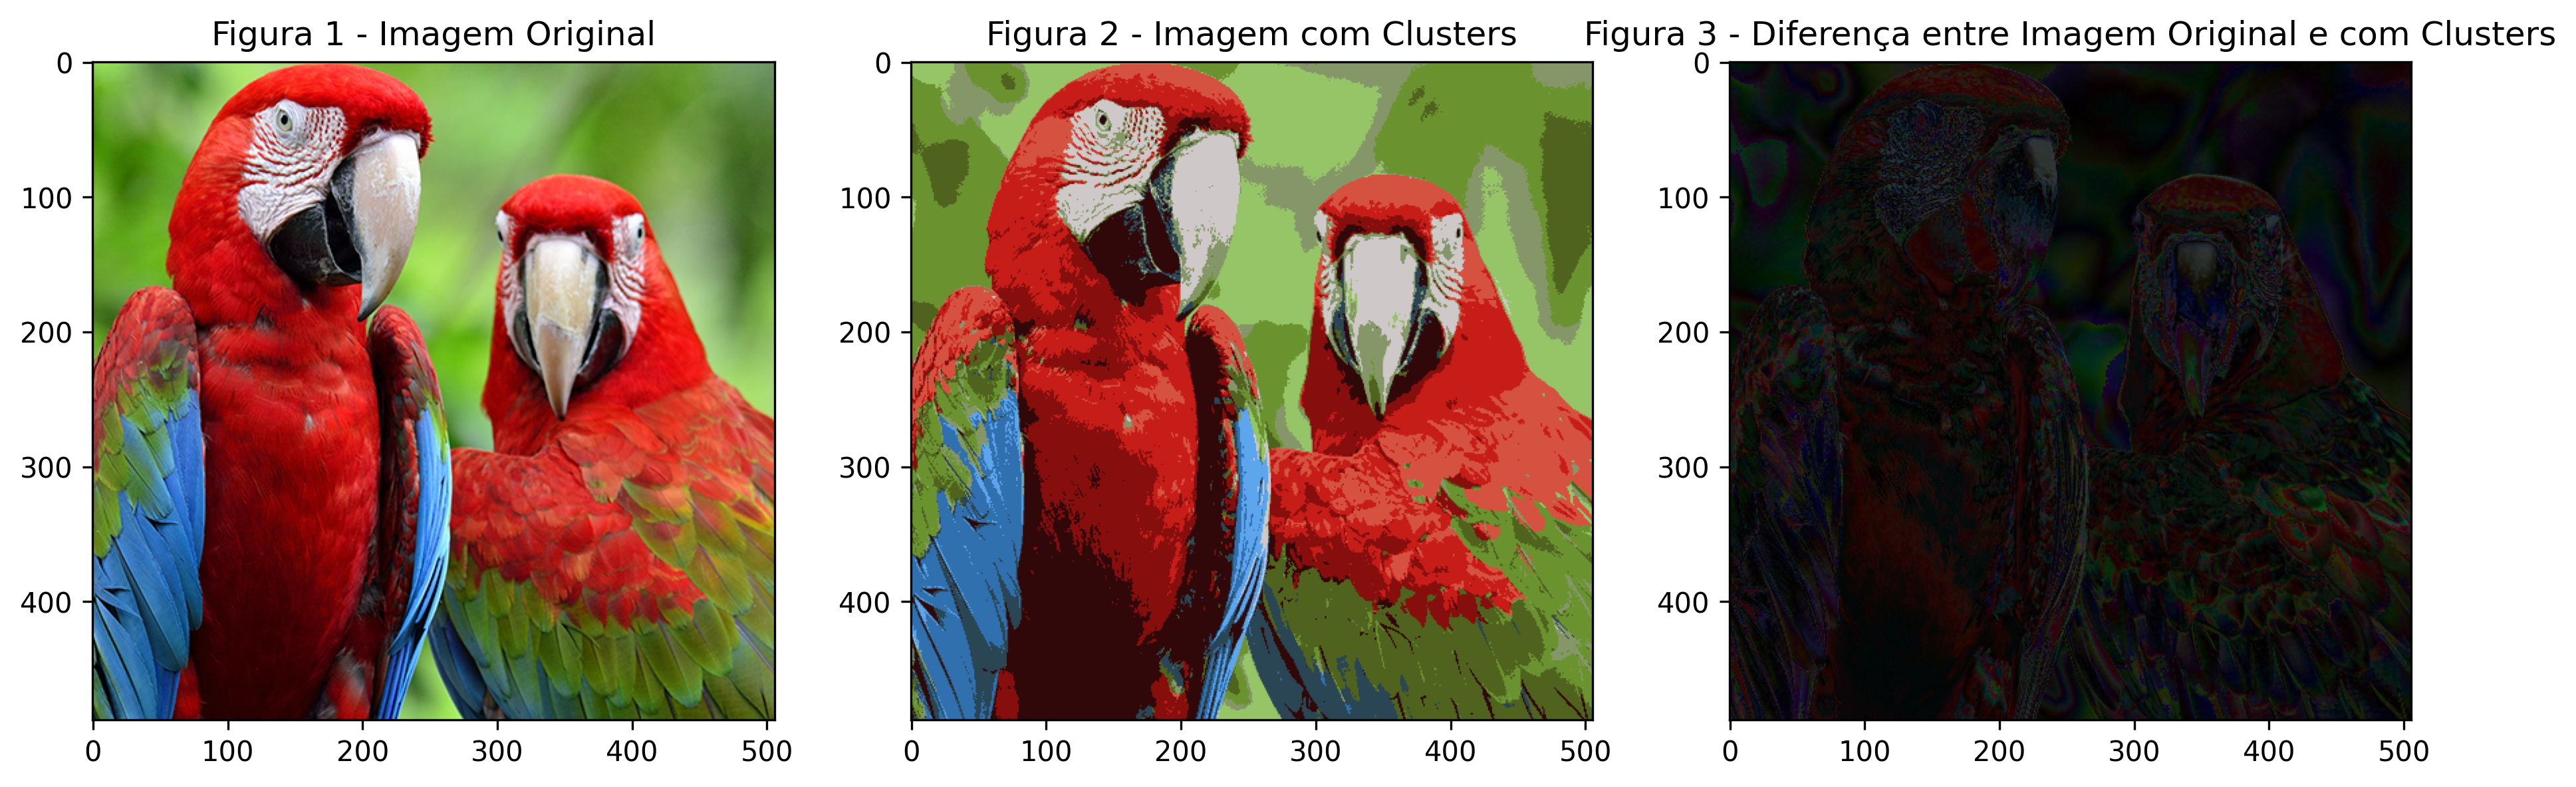
\includegraphics[width=0.9\textwidth]{../figures/5/optimal_k_result.png}
    \caption{Resultado com k=12 (valor otimizado)}
    \label{fig:optimal_k}
\end{figure}

A imagem acima apresenta o resultado da função \texttt{function\_1} para k=12, demonstrando que nesse ponto, a imagem mantém uma boa qualidade.
\newpage

\subsection*{Exercício 5e}
\addcontentsline{toc}{subsection}{Exercício 5e}


\begin{lstlisting}[language=Python]
def function_3(img):
    res = img.copy()
    for i in range(1, img.shape[0] - 1):
        for j in range(1, img.shape[1] - 1):
            up = (img[i, j] != img[i + 1, j]).any()
            down = (img[i, j] != img[i - 1, j]).any()
            left = (img[i, j] != img[i, j - 1]).any()
            right = (img[i, j] != img[i, j + 1]).any()
            if up or down or left or right:
                res[i, j] = np.array([0, 0, 0])  # Cor preta
    return res

# Aplicacao do algoritmo
output = function_1(imagem, 4)
edge = function_3(output)
\end{lstlisting}

\begin{figure}[H]
    \centering
    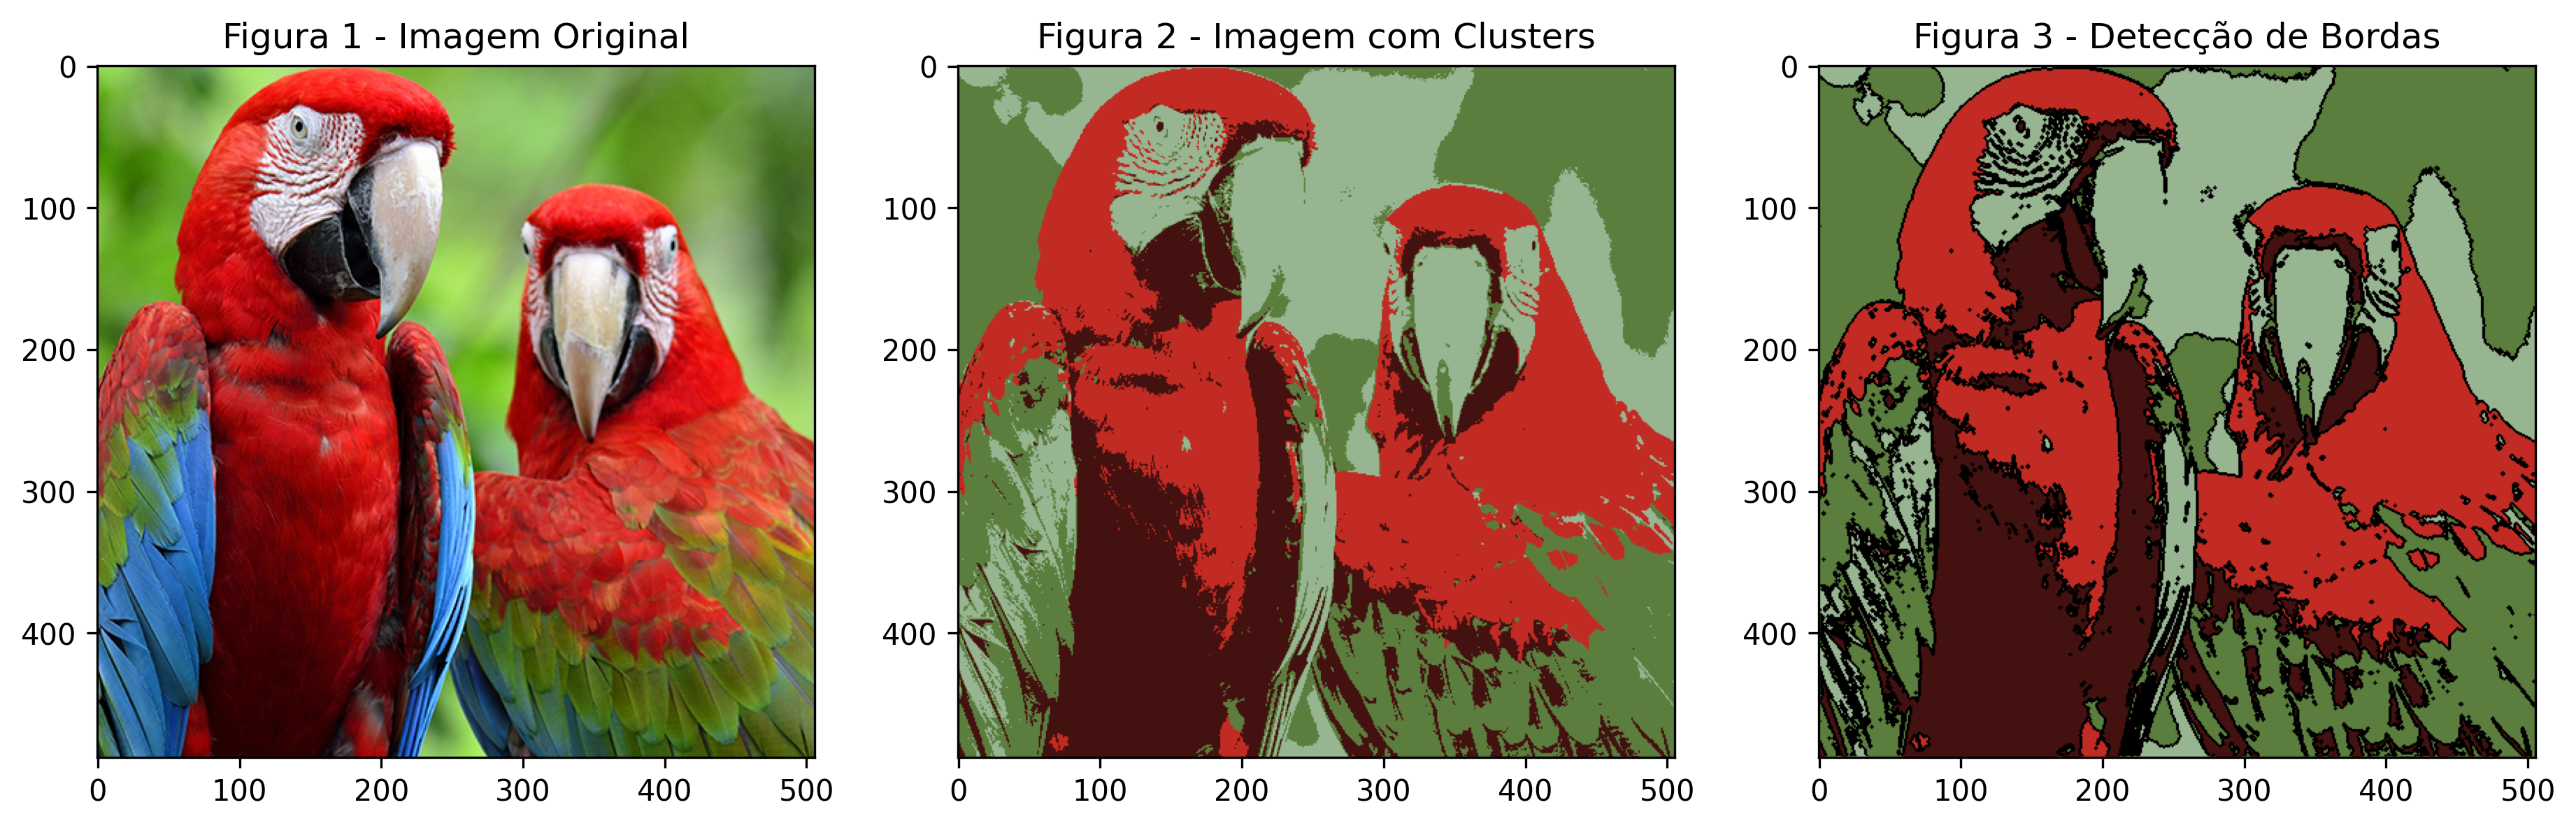
\includegraphics[width=0.9\textwidth]{../figures/5/edge_detection.png}
    \caption{Algoritmo de detecção de bordas baseado em clustering}
    \label{fig:edge_detection}
\end{figure}
\newpage

\subsection*{Exercício 5f}
\addcontentsline{toc}{subsection}{Exercício 5f}


Agora, além do vetor com as intensidades de vermelho, verde e azul, adicionamos também a coordenada x e y de cada pixel, com um certo peso w.

\begin{lstlisting}[language=Python]
def function_4(img, parameter, weight):
    tmp = img.copy()
    tmp = np.dstack((img, np.zeros((img.shape[0], img.shape[1]))))
    tmp = np.dstack((tmp, np.zeros((img.shape[0], img.shape[1]))))
    for i in range(tmp.shape[0]):
        for j in range(tmp.shape[1]):
            tmp[i, j, 3] = weight * i  # Coordenada x
            tmp[i, j, 4] = weight * j  # Coordenada y
    temp = np.reshape(tmp, (img.shape[0] * img.shape[1], 5))
    model = KMeans(n_clusters=parameter, random_state=0, n_init="auto").fit(temp)
    output = model.cluster_centers_[model.labels_]
    output = np.reshape(output, (img.shape[0], img.shape[1], 5))
    return output[:, :, :3]

# Teste com diferentes pesos
weights = [0, 0.001, 0.005, 0.0075, 0.01, 0.02, 0.05, 0.1, 1]
\end{lstlisting}

\begin{figure}[H]
    \centering
    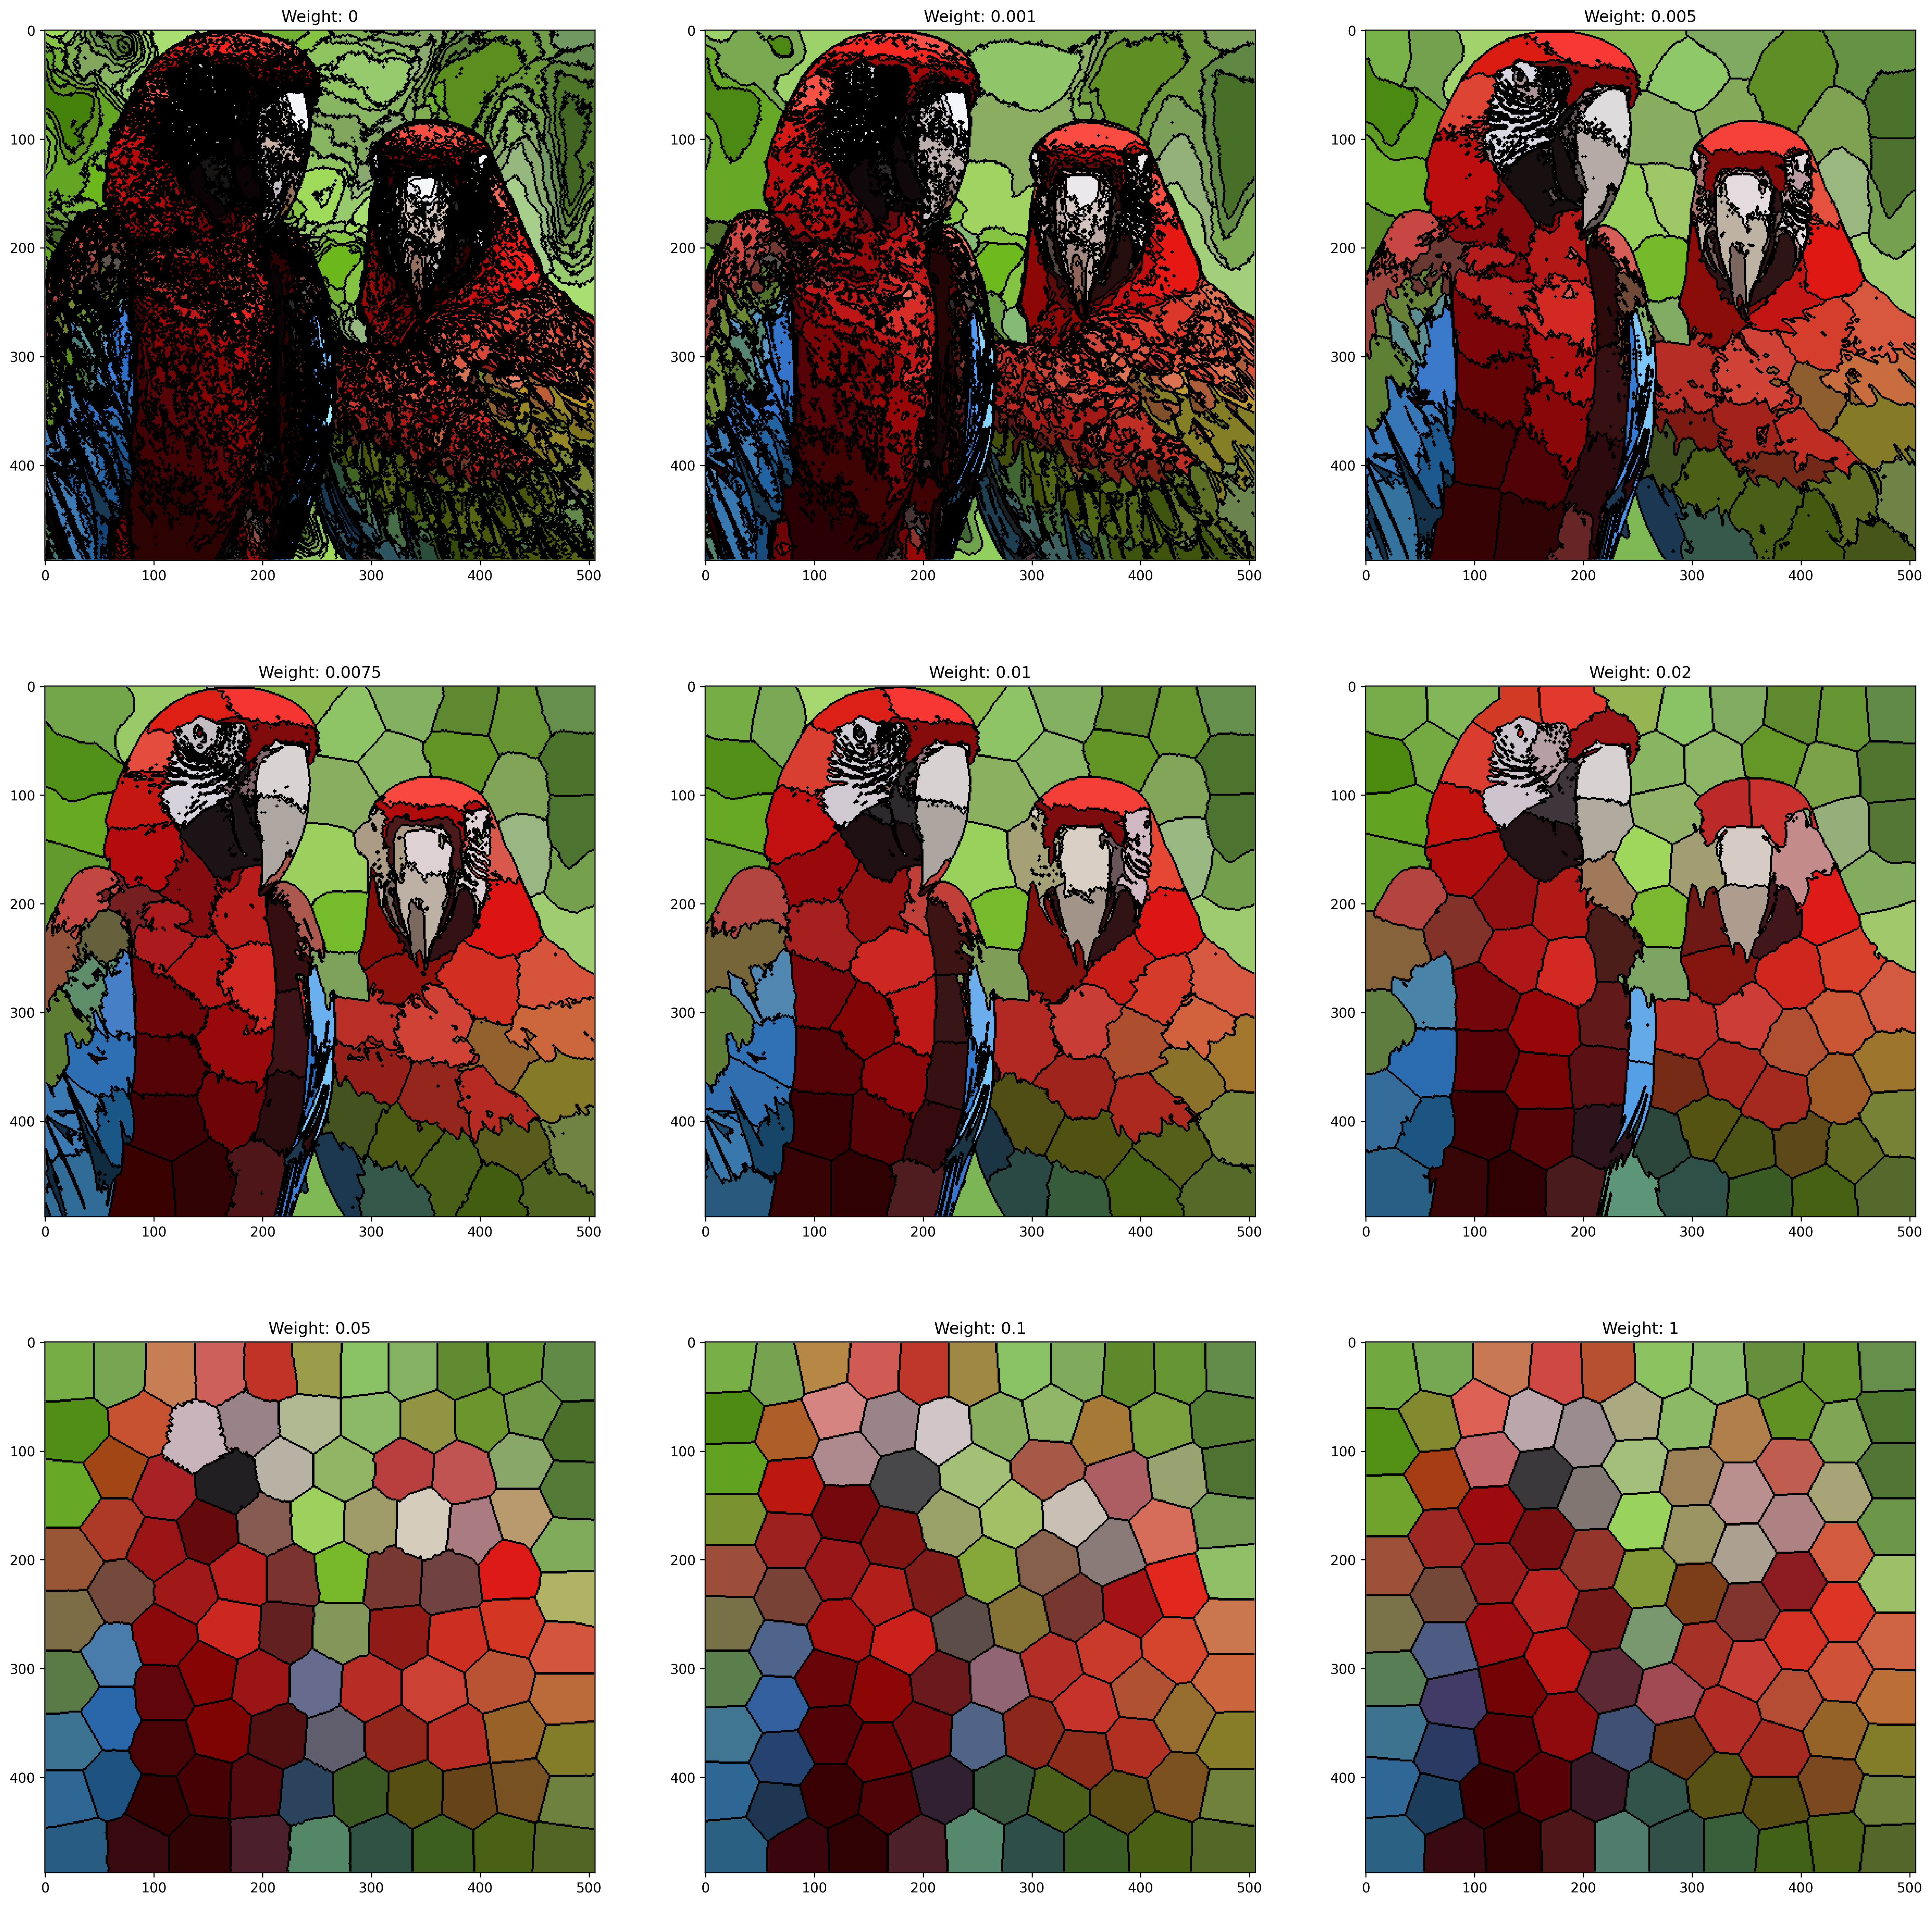
\includegraphics[width=0.9\textwidth]{../figures/5/weight_effects.png}
    \caption{Efeito do peso w na clusterização com coordenadas espaciais}
    \label{fig:weight_effects}
\end{figure}


A inclusão das coordenadas x e y adicionam informação espacial para o algoritmo de clusterização. Assim, além da similaridade das cores, ele também considerará
a proximidade entre os pixels. Os valores de w definem o quão sensível será o algoritmo à distância, de modo que valores pequenos de w fazem com que o método priorize
mais as cores, enquanto valores maiores dão enfoque na posição.

As figuras resultantes indicam exatamente isto. Para w = 0, temos o algoritmo original, apenas com cores, e para w maiores que 0.05, as cores praticamente não
importam, pois seus valores têm magnitude menor que a da posição de cada pixel. Nesta configuração, o contorno dos clusters é regular já que a fronteira entre os
grupos são basicamente os pontos equidistantes a dois ou, no caso das arestas entre três hexágonos, três centróides. Além disso, os centroides tendem a se organizar
em um formato regular, já que esta configuração seria mais adequada para aumentar a pureza entre os clusters.

\newpage


\end{document}